%& --translate-file=cp1250pl.tcx  %%%%%%%%%%%%%%

%% ----------------------------------------------------------------
%% Thesis.tex -- MAIN FILE (the one that you compile with LaTeX)
%% ---------------------------------------------------------------- 
% Set up the document
\documentclass[a4paper, 11pt, oneside]{Thesis} 
\graphicspath{{Figures/}{wykresy/}}
\newif\ifpdf
\ifx\pdfoutput\undefined
   \pdffalse
\else
   \pdfoutput=1
   \pdftrue
\fi
\ifpdf
   \usepackage{graphicx}
   \usepackage{epstopdf}
   \DeclareGraphicsRule{.eps}{pdf}{.pdf}{`epstopdf #1}
   \pdfcompresslevel=9
\else
   \usepackage{graphicx}
\fi
\usepackage{polski}
\usepackage{todonotes}
\usepackage{listing}
\lstset{ %
language=C++,                % choose the language of the code
basicstyle=\footnotesize,       % the size of the fonts that are used for the code
% showspaces=false,               % show spaces adding particular underscores
% showstringspaces=false,         % underline spaces within strings
% showtabs=false,                 % show tabs within strings adding particular underscores
% frame=single,                   % adds a frame around the code
% tabsize=2,                  % sets default tabsize to 2 spaces
% captionpos=b,                   % sets the caption-position to bottom
% breaklines=true,                % sets automatic line breaking
% breakatwhitespace=false,        % sets if automatic breaks should only happen at whitespace
escapeinside={\%*}{*)}          % if you want to add a comment within your code
}
\renewcommand{\lstlistlistingname}{Spis kod�w �r�d�owych} % Label of Table of Listings
\renewcommand{\lstlistingname}{Listing} % Label for every Listing

% Include any extra LaTeX packages required
\usepackage[square, numbers, comma, sort&compress]{natbib}  % Use the "Natbib" style for the references in the Bibliography
\usepackage{verbatim}  % Needed for the "comment" environment to make LaTeX comments
\usepackage{vector}  % Allows "\bvec{}" and "\buvec{}" for "blackboard" style bold vectors in maths
\hypersetup{urlcolor=blue, colorlinks=true}  % Colours hyperlinks in blue, but this can be distracting if there are many links.

\begin{document}
\frontmatter

\title  { Projekt i implementacja aplikacji realizuj�cej operacje arytmetyczne na kwantyfikatorach lingiwistycznych}
\authors  {\texorpdfstring{Bartosz Tacza�a}
            {Author Name}
            }
\addresses  {\groupname\\\deptname\\\univname} 

\maketitle

\addtotoc{Abstract}
\abstract{
\addtocontents{toc}{\vspace{1em}}

Analitic solution of decisive problems, based only on probabilities of event occurence, is extermally difficult and time-consuming and in most cases incorrect due to arithmetic exceptions made in progress of calculations. 
In This Master Thesis I will introduce author's application, capable of resolving those decision problems, by capably operating of probability distribution functions for probabilities given in problem. The main focus is on the methodology of solving such problem and as a particular example the problem of "Two business" is solved. 


}
\clearpage
\setstretch{1.3}  

\fancyhead{}
\rhead{\thepage}
\lhead{} 

\pagestyle{fancy}
\Declaration{
\addtocontents{toc}{\vspace{1em}}

O�wiadczam, ze przedk�adan� prac� magistersk� ko�cz�c� studia napisa�em samodzielnie.
Oznacza to, ze przy pisaniu pracy poza niezb�dnymi konsultacjami, nie korzysta�em
z pomocy innych os�b, a w szczeg�lno�ci nie zleca�em opracowania rozprawy lub
jej cz�ci innym osobom, ani nie odpisywa�em rozprawy lub jej cz�ci od innych os�b.
Potwierdzam tez zgodno�� wersji papierowej i elektronicznej z�o�onej pracy. Mam �wiadomo��,�e po�wiadczenie nieprawdy b�dzie w tym przypadku skutkowa�o cofni�ciem
decyzji o wydaniu dyplomu.

 
Podpis:\\
\rule[1em]{25em}{0.5pt}  % This prints a line for the signature
 
Data:\\
\rule[1em]{25em}{0.5pt}  % This prints a line to write the date
}
\clearpage  % Declaration ended, now start a new page

% The Abstract Page

\pagestyle{fancy}
\lhead{\emph{Spis tre�ci}}  
\tableofcontents  

%% ----------------------------------------------------------------
\lhead{\emph{Spis rysunk�w}}  % Set the left side page header to "List if Figures"
\listoffigures  

\addtotoc{Spis kod�w �r�d�owych}  % Add the "Abstract" page entry to the Contents
\lstlistoflistings
\clearpage  % Start a new page

%% ----------------------------------------------------------------
\setstretch{1.5}  % Set the line spacing to 1.5, this makes the following tables easier to read
\clearpage  % Start a new page
\lhead{\emph{Skr�ty}}  % Set the left side page header to "Abbreviations"
\listofsymbols{lll}  % Include a list of Abbreviations (a table of two columns)
{
    \textbf{STL} & \textbf{S}tandard \textbf{T}emplate \textbf{L}ibrary \\
    \textbf{GCC} & \textbf{G}nu \textbf{C}ommon \textbf{C}compilers \\
    \textbf{G++} & kompilator j�zyka C++ z pakietu GCC \\
    \textbf{MSVC} & \textbf{M}icro\textbf{S}oft \textbf{V}isual \textbf{C}++ \\
    \textbf{IDE} & \textbf{I}ntegrated \textbf{D}evelopment \textbf{E}nvironment
    \textbf{GDB} & \textbf{G}nu \textbf{D}e\textbf{b}ugger
}
\clearpage  %Start a new page
\lhead{\emph{Symbole}}  % Set the left side page header to "Symbols"
\listofnomenclature{lll}  % Include a list of Symbols (a three column table)
{
  $\oplus$ - Operacja dodowania kwantyfikator�w lingwistycznych \\
  $\ominus$ - Operacja odejmowania kwantyfikator�w lingwistycznych\\
  $\otimes$ - Operacja mno�enia kwantyfikator�w lingwistycznych\\
  $\oslash$ - Operacja dzielenia kwantyfikator�w lingwistycznych \\
}
\setstretch{1.3} 

%% ----------------------------------------------------------------
\mainmatter
\pagestyle{fancy}

% Wprowadzenie, rozdzia� 1 
\chapter{Wprowadzenie} 
\label{Rozdzia� 1 }
\lhead{Rozdzia� 1. \emph{Tematyka pracy }} 


\section{Tematyka pracy}

Welcome to this ``\LaTeX{} Thesis Template'', a beautiful and easy to use template for writing a thesis using the \LaTeX{} typesetting system.

If you are writing a thesis (or will be in the future) and its subject is technical or mathematical (though it doesn't have to be), then creating it in \LaTeX{} is highly recommended as a way to make sure you can just get down to the essential writing without having to worry over formatting or wasting time arguing with your word processor.

\LaTeX{} is easily able to professionally typeset documents that run to hundreds or thousands of pages long. With simple mark-up commands, it automatically sets out the table of contents, margins, page headers and footers and keeps the formatting consistent and beautiful. One of its main strengths is the way it can easily typeset mathematics, even \emph{heavy} mathematics. Even if those equations are the most horribly twisted and most difficult mathematical problems that can only be solved on a super-computer, you can at least count on \LaTeX{} to make them look stunning.


\section{Motywacja}

\LaTeX{} is not a WYSIWYG (What You See is What You Get) program, unlike word processors such as Microsoft Word or Corel WordPerfect. Instead, a document written for \LaTeX{} is actually a simple, plain text file that contains \emph{no formatting}. You tell \LaTeX{} how you want the formatting in the finished document by writing in simple commands amongst the text, for example, if I want to use \emph{italic text for emphasis}, I write the `$\backslash$\texttt{emph}\{\}' command and put the text I want in italics in between the curly braces. This means that \LaTeX{} is a ``mark-up'' language, very much like HTML.



\section{Cel pracy}

If you are familiar with \LaTeX{}, then you can familiarise yourself with the contents of the \href{http://www.sunilpatel.co.uk/files/Thesis\%20Template.zip}{Zip file} and the directory structure and then place your own information into the `\texttt{Thesis.cls}' file. Section \ref{FillingFile} on page \pageref{FillingFile} tells you how to do this. Make sure you read section \ref{ThesisConventions} about thesis conventions to get the most out of this template and then get started with the `\texttt{Thesis.tex}' file straightaway.

If you are new to \LaTeX{} it is recommended that you carry on reading through the rest of the information in this document.

\section{Realizacja}

If you are familiar with \LaTeX{}, then you can familiarise yourself with the contents of the \href{http://www.sunilpatel.co.uk/files/Thesis\%20Template.zip}{Zip file} and the directory structure and then place your own information into the `\texttt{Thesis.cls}' file. Section \ref{FillingFile} on page \pageref{FillingFile} tells you how to do this. Make sure you read section \ref{ThesisConventions} about thesis conventions to get the most out of this template and then get started with the `\texttt{Thesis.tex}' file straightaway.

If you are new to \LaTeX{} it is recommended that you carry on reading through the rest of the information in this document.

\section{Implementacja}

If you are familiar with \LaTeX{}, then you can familiarise yourself with the contents of the \href{http://www.sunilpatel.co.uk/files/Thesis\%20Template.zip}{Zip file} and the directory structure and then place your own information into the `\texttt{Thesis.cls}' file. Section \ref{FillingFile} on page \pageref{FillingFile} tells you how to do this. Make sure you read section \ref{ThesisConventions} about thesis conventions to get the most out of this template and then get started with the `\texttt{Thesis.tex}' file straightaway.

If you are new to \LaTeX{} it is recommended that you carry on reading through the rest of the information in this document.

 
% Wprowadzenie, rozdzia� 1 
\chapter{Cz�� teoretyczna} 
\label{Rozdzia� 2 }
\lhead{Rozdzia� 2. \emph{Cz�� teoretyczna }} 


\section{Wyja�nienie podstawowych zagadnie� z zakresu statystyki matematycznej}

\section{Funkcja g�sto�ci oraz jej w�a�ciwo�ci}

\section{Czym jest splot funkcji oraz jak� rol� pe�ni w statystyce matematycznej}
\subsection{Definicja splotu funkcji}
\subsection{W�a�no�ci splotu funkcji}
\subsection{R�ne sploty funkcji, oraz ich wykresy}

\section{Wyja�nienie podstawowych zagadnie� z zakresu matematyki rozmytej}
\subsection{nCzy s� kwantyfikatory lingwistyczne oraz na czym polega rozmywanie wiedzy}
\subsection{Dlaczego kwantyfikator lingwistyczny mo�na przedstawi� jako funkcj� rozk�adu g�sto�ci prawdopodobie�stwa?}

\section{Centralne twierdzenie graniczne}

 
% Wprowadzenie, rozdzia� 1 
\chapter{Cz�� praktyczna} 
\label{Rozdzia� 3 }
\lhead{Rozdzia� 3. \emph{Cz�� praktyczna }} 


\section{Opis za�o�e� programu}

\subsection{Co ma program robi�, w jakich �rodowiska dzia�a�. }

\section{Opis technologi u�ytych przy tworzeniu oprogramowania}
\subsection{J�zyk, �rodowisko}
\subsection{Opis bibliotek zewn�trznych}

\section{Struktura programu}
\subsection{Opis modu��w u�ytych w programie}
\subsubsection{Szczeg�owy opis biblioteki fl ( jakie funkcje itd ) }
\subsubsection{Opis parsera matematycznego}
\subsubsection{Opis biblioteki do rysowania funkcji}
\subsection{Jak to si� wszystko zaz�bia ( rysunki pewnie ) }


\section{Opis mo�liwo�ci programu }

\section{Przyk�adowe u�ycie}

 
% Wprowadzenie, rozdzia� 1 
\chapter{Rozwi�zanie przyk�adowego zadania} 
\label{Rozdzia� 4 }
\lhead{Rozdzia� 4. \emph{Rozwi�zanie przyk�adowego zadania }} 
\section{Postawienie zadania}
Zadaniem, kt�re zostanie rozwi�zane za pomoc� programu b�d�cego podmiotem pracy magisterskiej, jest problem "dw�ch biznes�w". Jest to problem decyzyjny, w kt�rym nale�y poda� rozwi�zanie opieraj�c si� jedynie na informacjach, podanych w j�zyku naturalnym, przedstawionych jako kwantyfikatory lingwistyczne.  
Problem postawiony jest nast�puj�co:

\begin{quote}
W biznesie $B_1$ mo�na zarobi� od 0 do 10 milion�w z�otych. Prawdopodobie�stwo dochodu bliskiego 10 milion�w z�otych jest du�e. 
W biznesie $B_2$ mo�na zarobi� od 0 do 20 milion�w z�otych. Prawdopodobie�stwo dochodu bliskiego 20 milion�w z�otych jest jednak ma�e. \newline Decyzja: W
kt�ry z biznes�w zainwestowa�?
\end{quote}

Rozwi�zaniem tego problemu s� warto�ci oczekiwane dochod�w obu biznes�w. Aby jednak te warto�ci obliczy� nale�y znale�� rozk�ady prawdopodobie�stwa dla obu biznes�w. W rozdziale 2 przedstawi�em w jaki spos�b ��czy� kwantyfikatora z rozk�adem prawdopodobie�stwa, teraz wykorzystamy ten fakt w celu rozpisania funkcji g�sto�ci rozk�ad�w. 
Zmienna losowa ci�g�a dla obu biznes�w wygl�da nast�puj�co:
\begin{equation}
 S_N = PR_N*DB_n + NIEPR_N * NIEDB_N, 
\end{equation}
gdzie:
\begin{itemize}
 \item $S_N$ - zmienna losowa dla biznesu n-tego,
 \item $PR_N$ - oznacza zmienn� losow� prawdopodobie�stwa osi�gni�cia dochodu $DB_N$,
 \item $DB_N$ - oznacza zmienn� losow� okre�laj�c� doch�d z biznesu n-tego,
 \item $NIEPR_N$ - oznacza zmienn� losow� przeciwn� do $PR_N$, czyli przeciwne prawdopodobie�stwo osi�gni�cia dochodu przeciwnego,
 \item $NIEDB_N$ - oznacza zmienn� losow� okre�laj�c� przeciwny doch�d z biznesu n-tego.
\end{itemize}
Operacje + i * na zmiennych losowych uto�samiamy z operacjami $\oplus$  oraz $\otimes$ na ich rozk�adach. 
\section{Identyfikacja funkcji g�sto�ci }
Aby podej�� do pr�by rozwi�zania tego problemu nale�y okre�li� kwantyfikatory lingwistyczne
\begin{itemize}
\item {du�e},
\item {ma�e ( nie du�e ) },
\item {bliskie, dla warto�ci maksymalnej dochodu z biznesu pierwszego },
\item {nie bliskie , dla warto�ci maksymalnej dochodu z biznesu pierwszego },
\item {bliskie, dla warto�ci maksymalnej dochodu z biznesu drugiego },
\item {nie bliskie , dla warto�ci maksymalnej dochodu z biznesu drugiego}.
\end{itemize}
oraz odpowiadaj�ce im funkcje rozk�adu g�sto�ci. 
Kwantyfikatory \emph{du�e} i \emph{ma�e}, zostan� okre�lone na podstawie pracy doktora Marka Landowskiego \cite{landowski_d}. 
Doktor po przeprowadzeniu ankiety wy�uska� dane dotycz�ce oznaczania danej warto�ci prawdopodobie�stwa jako du�ej, ma�ej oraz �redniej. W naszym przypadku, interesuj� nas tylko badania odno�nie pojmowania prawdopodobie�stwa jako du�ego oraz ma�ego. 
Kwantyfikatory uzyskane przez doktora Marka Landowskiego pos�u�� nam do okre�lenia funkcji rozk�adu g�sto�ci prawdopodobie�stwa. 
Kwantyfikatory \emph{bliskie 10 mln}, \emph{nie bliskie 10 mln}, \emph{bliskie 20 mln} oraz \emph{nie bliskie 20 mln} s� okre�lone poprzez rozci�gniecie kwantyfikator�w \emph{ma�e} i \emph{du�e} na przedzia�y im odpowiadaj�ce. \footnote{ np. \emph{bliskie 10 mln} na przedzia� $[0,10]$}
Dane otrzymane przez doktora Landowskiego ,mo�na przybli�y� funkcjami wysokich rz�d�w, ale punkty uk�adaj� si� w spos�b pozwalaj�cy przeprowadzi� aproksymacj� funkcjami pierwszego i zerowego rz�du ( funkcjami liniowymi oraz
funkcjami sta�ymi ), bez du�ej straty dok�adno�ci, co pokazano na rysunkach \ref{wykres:duze_kropki_aproksymacja} \ref{wykres:male_kropki_aproksymacja}.Aby zachowa� pewne ustalenie, pozosta�e kwantyfikatory r�wnie� b�d� mia�y posta� funkcji pierwszego i zerowego rz�du. W
Aby zidentyfikowa� poszczeg�lne funkcje rozk�adu g�sto�ci prawdopodobie�stwa nale�y przypatrze� si� rozk�adowi punkt�w dla danego kwantyfikatora, oraz wykorzystuj�c w�a�ciwo�� ca�kowania do jedno�ci funkcji g�sto�ci na okre�lonym przedziale, rozwi�za� uk�ad r�wna�, kt�ry okre�li nam funkcj� pierwszego rz�du oraz maksymaln� wysoko�� funkcji rozk�adu prawdopodobie�stwa ( maksymalna wysoko�� kwantyfikator�w wynosi 1, jednak w naszym przypadku, wysoko�� trzeba przeskalowa�, aby uzyska� funkcj� ca�kuj�c� si� do jedno�ci ). 
Ca�y algorytm aproksymacji zostanie przedstawiony dla kwantyfikatora \emph{du�e}, natomiast dla reszty kwantyfikator�w pomini�te zostan� obliczenia i przedstawione zostan� tylko wyniki. W
W poni�szych obliczeniach o� rz�dnych oznacza warto�� prawdopodobie�stwa, dla kwantyfikator�w \emph{du�e} i \emph{ma�e}, oraz warto�� dochodu dla kwantyfikator�w \emph{bliskie 10 mln}, \emph{nie bliskie 10 mln}, \emph{bliskie 20 mln} oraz \emph{nie bliskie 20 mln}.
\subsection{Kwantyfikator "du�e"}
\begin{figure}[ht]
    \centering
    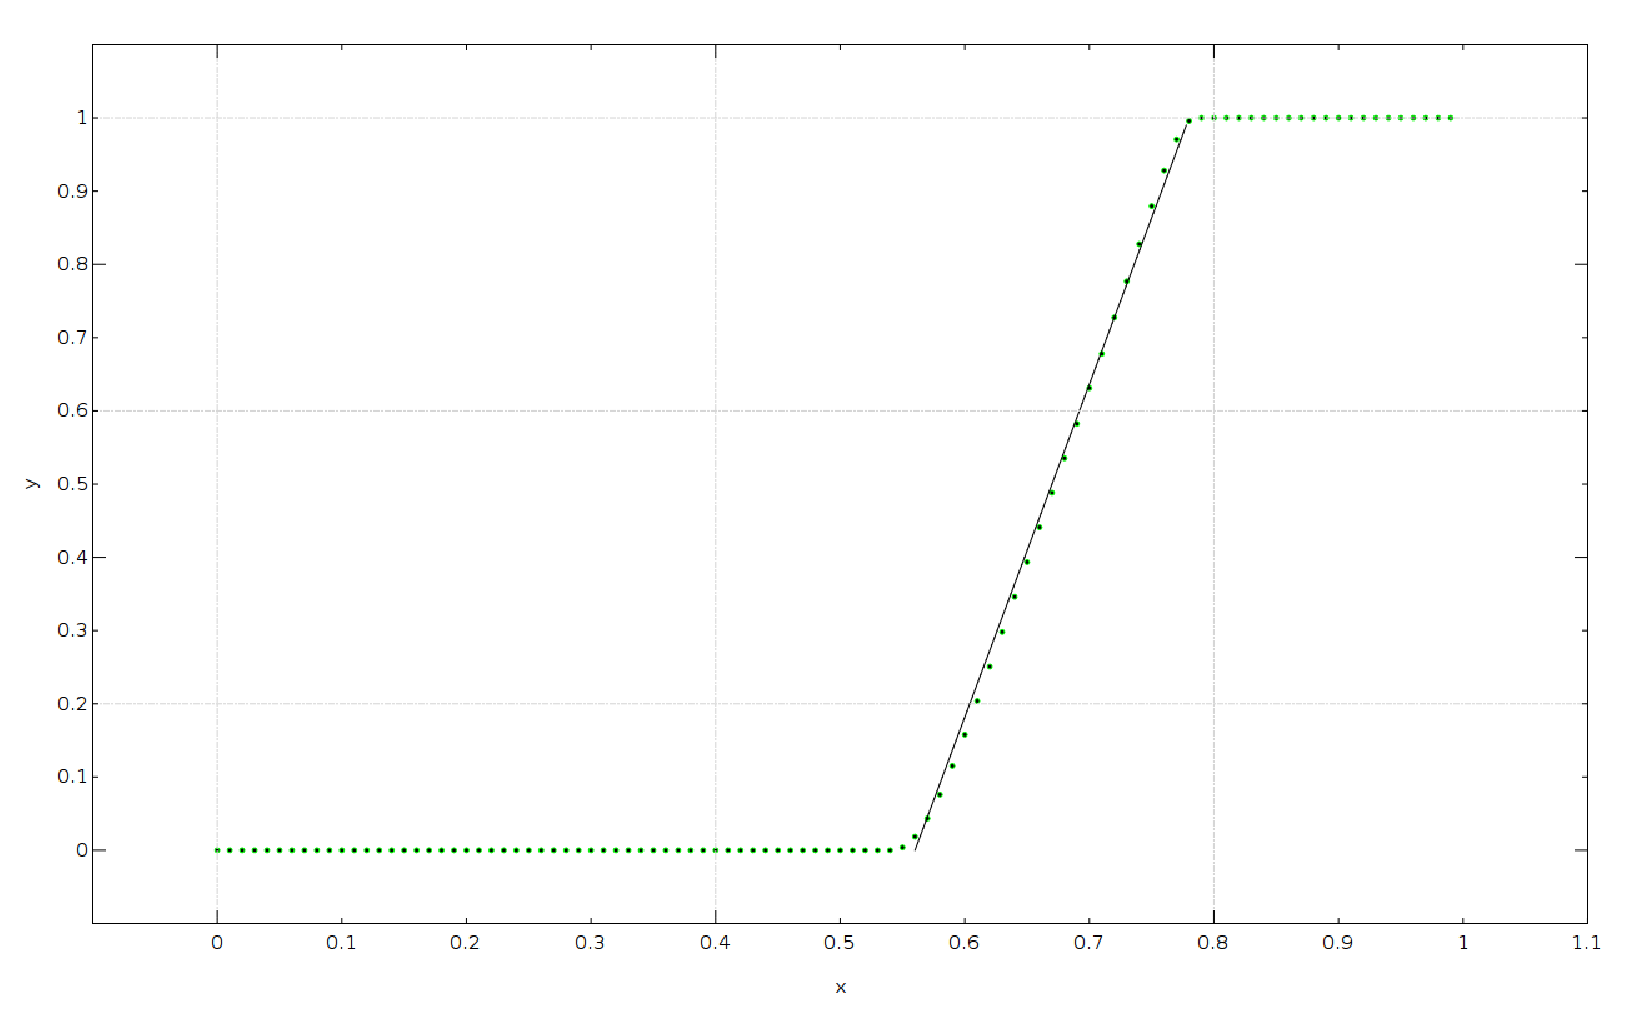
\includegraphics[width=15cm]{duze_kropki_aproksymacja.eps}
      \rule{35em}{0.5pt}
    \caption[Wykres kwantyfikatora du�e]{Wykres punkt�w zebranych dla kwantyfikatora \emph{du�e}}
    \label{wykres:duze_kropki_aproksymacja}
\end{figure}
Mamy dany zbi�r punkt�w, przedstawiony na wykresie \ref{wykres:duze_kropki_aproksymacja} i dla tego zbioru, trzeba oszacowa� funkcj� rozk�adu g�sto�ci prawdopodobie�stwa. Aby to uczyni� trzeba odczyta� z wykresu punkty gdzie funkcja zaczyna zmienia� swoj� posta�. W punkcie [0.56,0] funkcja zaczyna rosn��, w punkcie [0.78,1] funkcja zmienia swoj� charakterystyk� z liniowej na sta��. Tak wi�c nasza szukana funkcja b�dzie w przedziale 0 - 0.56 sta�a, w przedziale 0.56 - 0.78 przyjmie posta� funkcji liniowej, a w przedziale 0.78 - 1 znowu zmienia si� w funkcj� sta��. Na rysunku zaznaczono r�wnie�, jak dobrze funkcja liniowa pokrywa si� z punktami z przedzia�u 0.56 - 0.78 i �e jest ona wystarczaj�ca do aproksymacji. 
Przy aproksymacji nale�y pami�ta�, �e o ile warto�� maksymalna kwantyfikatora wynosi 1 ( jaka� warto�� przynale�y do kwantyfikatora w stopniu maksymalnym ), to zaaproksymowana na jej podstawie funkcja g�sto�ci warto�� maksymaln� b�dzie mia�a przeskalowan� tak, aby mog�a si� ca�kowa� do jedno�ci. 
Szukana funkcja b�dzie mia�a zatem posta�:
\begin{equation}
\label{rownanie:duze_wzor}
f(x) = \left\{ 
\begin{array}{l l}
  ax+b, & \quad \text{ dla 0.56 $<$ $x$ $\leq$ 0.78}\\
  c, & \quad \text{ dla 0.78 $<$ $x$ $<$ 1} .
\end{array} \right.
\end{equation}
Aby znale�� sta�e $a$, $b$ oraz $c$ rozwi�zujemy uk�ad r�wna�:
\begin{equation}
\label{uklad_rownan:duze_ur}
\begin{cases}
(1-0.78)*c + \frac{1}{2}*(0.78-0.56)*c = 1\\
0.56*a + b = 0  \\
0.78*a + b = c \\
\end{cases}
\Rightarrow \;
\begin{cases}
0*a + 0*b + 0.33*c = 1\\
0.56*a + 1*b + 0*c = 0\\
0.78*a + 1*b - 1*c = 0.
\end{cases}
\end{equation}
Pierwsze r�wnanie z uk�adu \ref{uklad_rownan:duze_ur} wynika z faktu, �e funkcja rozk�adu g�sto�ci prawdopodobie�stwa musi si� ca�kowa� do jedno�ci na ca�ym przedziale. (Poza przedzia�em 0.56 - 1 funkcja jest nieokre�lona, co oznacza, �e pole pod wykresem poza tym przedzia�em jest r�wne 0 i nie musi by� brane pod uwag�)
Kolejne dwa  r�wnania z uk�adu \ref{uklad_rownan:duze_ur} wynikaj� z rozpi�cia funkcji liniowej mi�dzy punktami (0.56 , 0) oraz (0.78  ,$c$). 
Trzecie
Uk�ad r�wna�, przekszta�camy do r�wnania macierzowego:
\begin{equation}
\label{rownanie:duze_macierz}
 \begin{bmatrix} 
 0 & 0 & 0.33 \\ 
 0.56 & 1 & 0 \\
 0.78 & 1 & -1 \\
 \end{bmatrix}
 * 
 \begin{bmatrix} 
 a \\ 
 b \\
 c \\
 \end{bmatrix}
 = 
 \begin{bmatrix} 
 1 \\ 
 0 \\
 0 \\
 \end{bmatrix}, 
\end{equation} 
co po przekszta�ceniu daje r�wnanie:
\begin{equation}
\label{rownanie:duze_mnozenie_macierzy} 
 \begin{bmatrix} 
 a \\ 
 b \\
 c \\
 \end{bmatrix}
 = 
 {\begin{bmatrix} 
 0 & 0 & 0.33 \\ 
 0.56 & 1 & 0 \\
 0.78 & 1 & -1 \\
 \end{bmatrix}}^{-1}
 *
 \begin{bmatrix} 
 1 \\ 
 0 \\
 0 \\
 \end{bmatrix}.
\end{equation} 
Rozwi�zanie tego r�wnania macierzowego wynosi:
\begin{equation}
 a = 13.774,
 b = -7.713
 c = 3.030.
\end{equation}
\begin{figure}[ht]
    \centering
    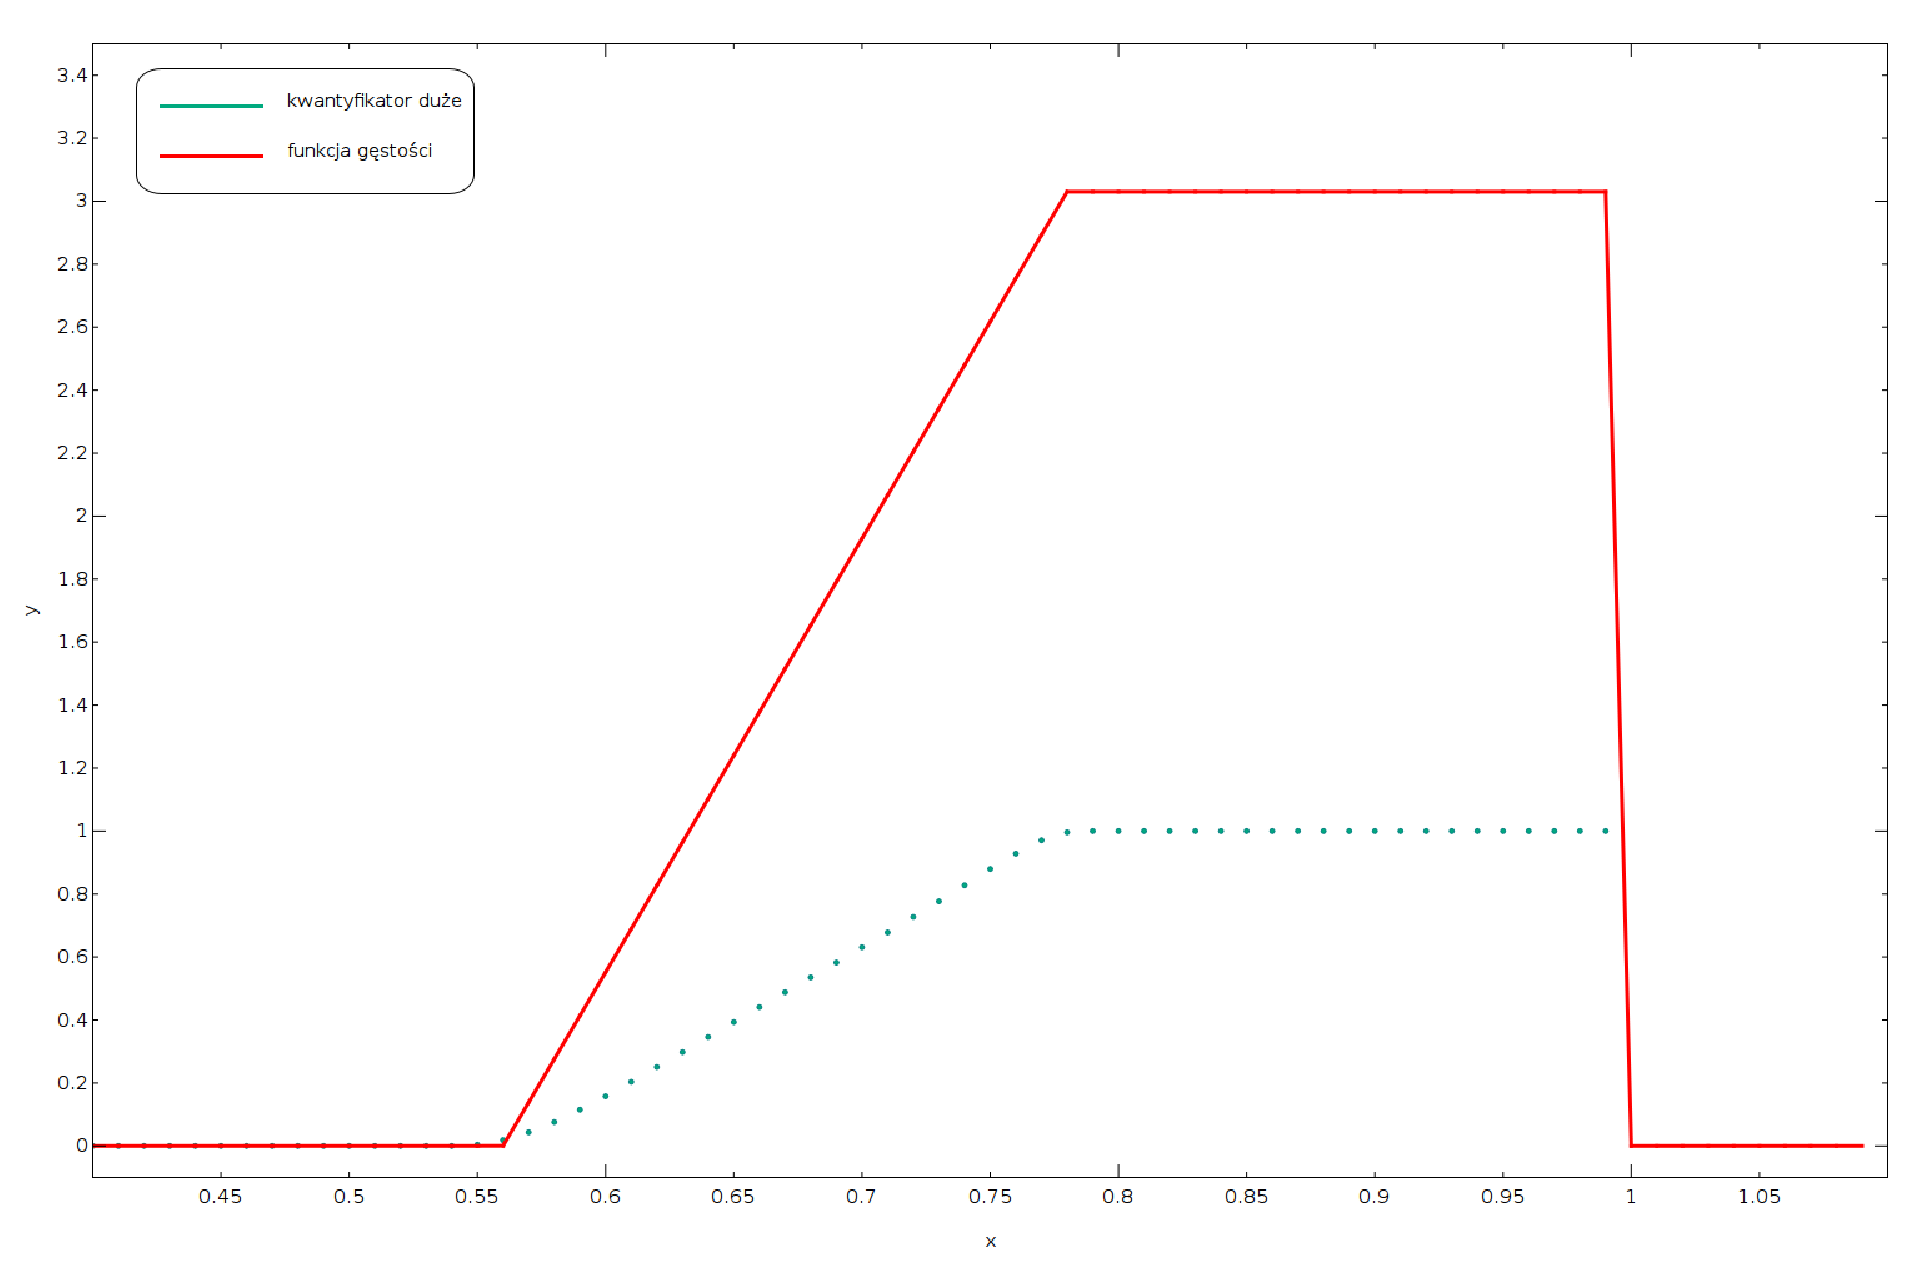
\includegraphics[width=15cm]{duze_kwantyfikator_aproksymacja.eps}
      \rule{35em}{0.5pt}
    \caption[Wykres kwantyfikatora \emph{du�e} wraz z odpowiadaj�c� mu funkcj� rozk�adu g�sto�ci prawdopodobie�stwa]{Wykres kwantyfikatora \emph{du�e} wraz z funkcj� rozk�adu g�sto�ci prawdopodobie�stwa}
    \label{wykres:duze_kwantyfikator_wraz_z_aproksymacja}
\end{figure}
Funkcja rozk�adu g�sto�ci prawdopodobie�stwa, dla kwantyfikatora \emph{du�e}, pokazana na rysunku \ref{wykres:duze_kwantyfikator_wraz_z_aproksymacja} wraz z kwantyfikatorem, ma nast�puj�cy wz�r:
\begin{equation}
\label{rownanie:duze_wynik}
f(x) = \left\{ 
\begin{array}{l l}
  10.331*x - 5.785, & \quad \text{ dla 0.56 $<$ $x$ $\leq$ 0.78}\\
  2.273, & \quad \text{ dla 0.78 $<$ $x$ $<=$ 1}.
\end{array}\right.
\end{equation}
\subsection{Kwantyfikator "ma�e"}
\begin{figure}[ht]
    
    \centering
    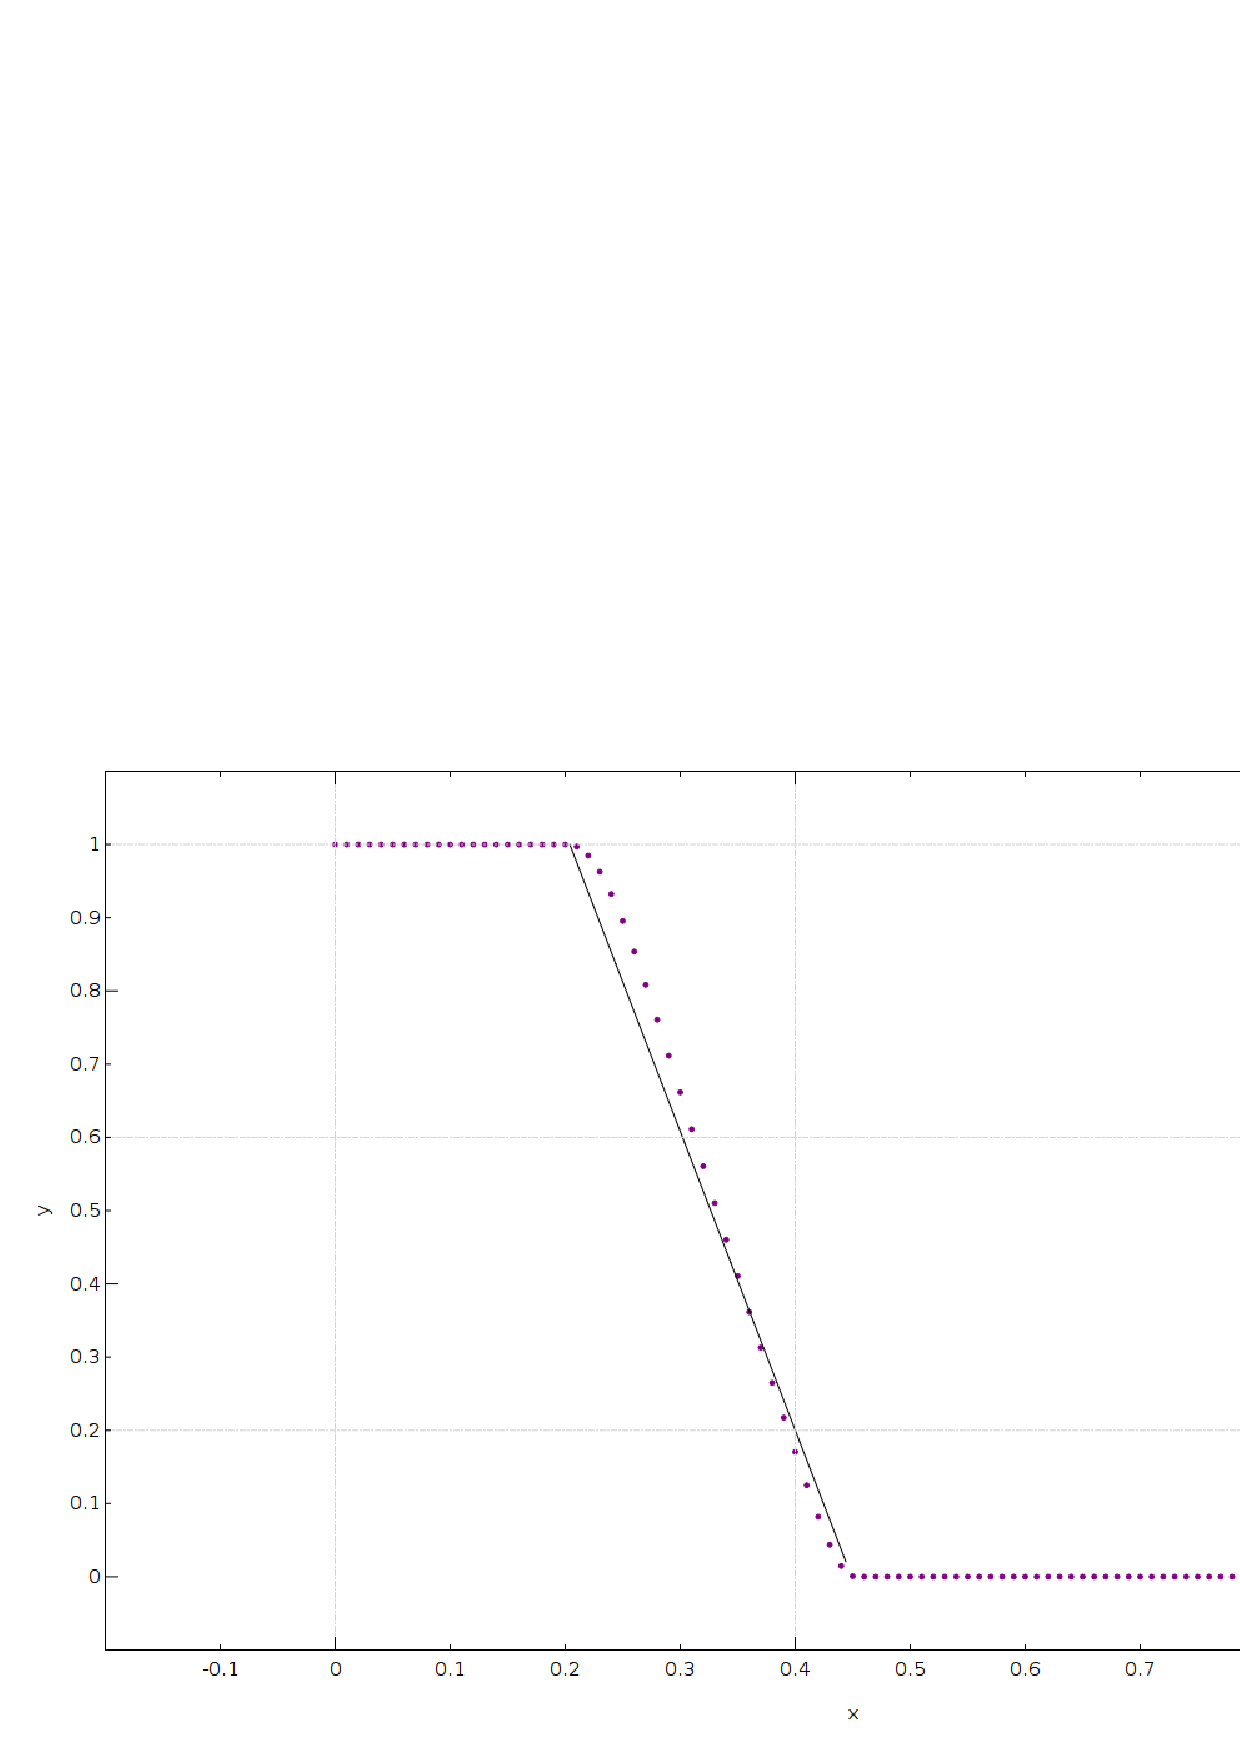
\includegraphics[width=15cm]{male_kropki_aproksymacja.pdf}
      \rule{35em}{0.5pt}
    \caption[Wykres kwantyfikatora ma�e]{Wykres punkt�w zebranych dla kwantyfikatora \emph{ma�e}}
    \label{wykres:male_kropki_aproksymacja}
\end{figure}
Mamy dany zbi�r punkt�w, przedstawiony na wykresie \ref{wykres:male_kropki_aproksymacja} i analogicznie trzeba oszacowa� funkcj� rozk�adu g�sto�ci prawdopodobie�stwa. Odczytujemy z wykresu punkty gdzie funkcja zaczyna zmienia� swoj� posta�. W punkcie [0.204,0] funkcja zaczyna male�, w punkcie [0.454,1] funkcja zmienia swoj� charakterystyk� z liniowej na sta��. Tak wi�c nasza szukana funkcja b�dzie w przedziale 0 - 0.204 sta�a, w przedziale 0. - 0.454 przyjmie posta� funkcji liniowej, a w przedziale 0.454 - 1 znowu zmienia si� w funkcj� sta��. 
Aproksymowana funkcja b�dzie postaci podobnej do funkcji g�sto�ci dla kwantyfikatora \emph{du�e} opisanej wzorem \ref{rownanie:duze_wzor} : 
\begin{equation}
\label{rownanie:male_wzor}
f(x) = \left\{ 
\begin{array}{l l}
  ax+b, & \quad \text{ dla 0.204 $<$ $x$ $\leq$ 0.454}\\
  c, & \quad \text{ dla 0 $<$ $x$ $<$ 0.204} .
\end{array} \right.
\end{equation}
Aby obliczy� $a$, $b$ oraz $c$ rozwi�zujemy uk�ad analogiczny do uk�adu r�wna� \ref{uklad_rownan:duze_ur}. 
Ko�cowe operacja jest analogiczna do mno�enia macierzy \ref{rownanie:duze_mnozenie_macierzy}, i wygl�da nast�puj�co:
\begin{equation}
\label{rownanie:male_mnozenie_macierzy} 
 \begin{bmatrix} 
 a \\ 
 b \\
 c \\
 \end{bmatrix}
 = 
 {\begin{bmatrix} 
 0 & 0 & 0.33 \\ 
 0.455 & 1 & 0 \\
 0.204 & 1 & -1 \\
 \end{bmatrix}}^{-1}
 *
 \begin{bmatrix} 
 1 \\ 
 0 \\
 0 \\
 \end{bmatrix}, 
\end{equation} 
a rozwi�zaniem tego uk�adu jest tr�jka:
\begin{equation}
 a = -8.775, 
 b = 3.993,  
 c = 2.203.
\end{equation} 
\begin{figure}[ht]
    
    \centering
    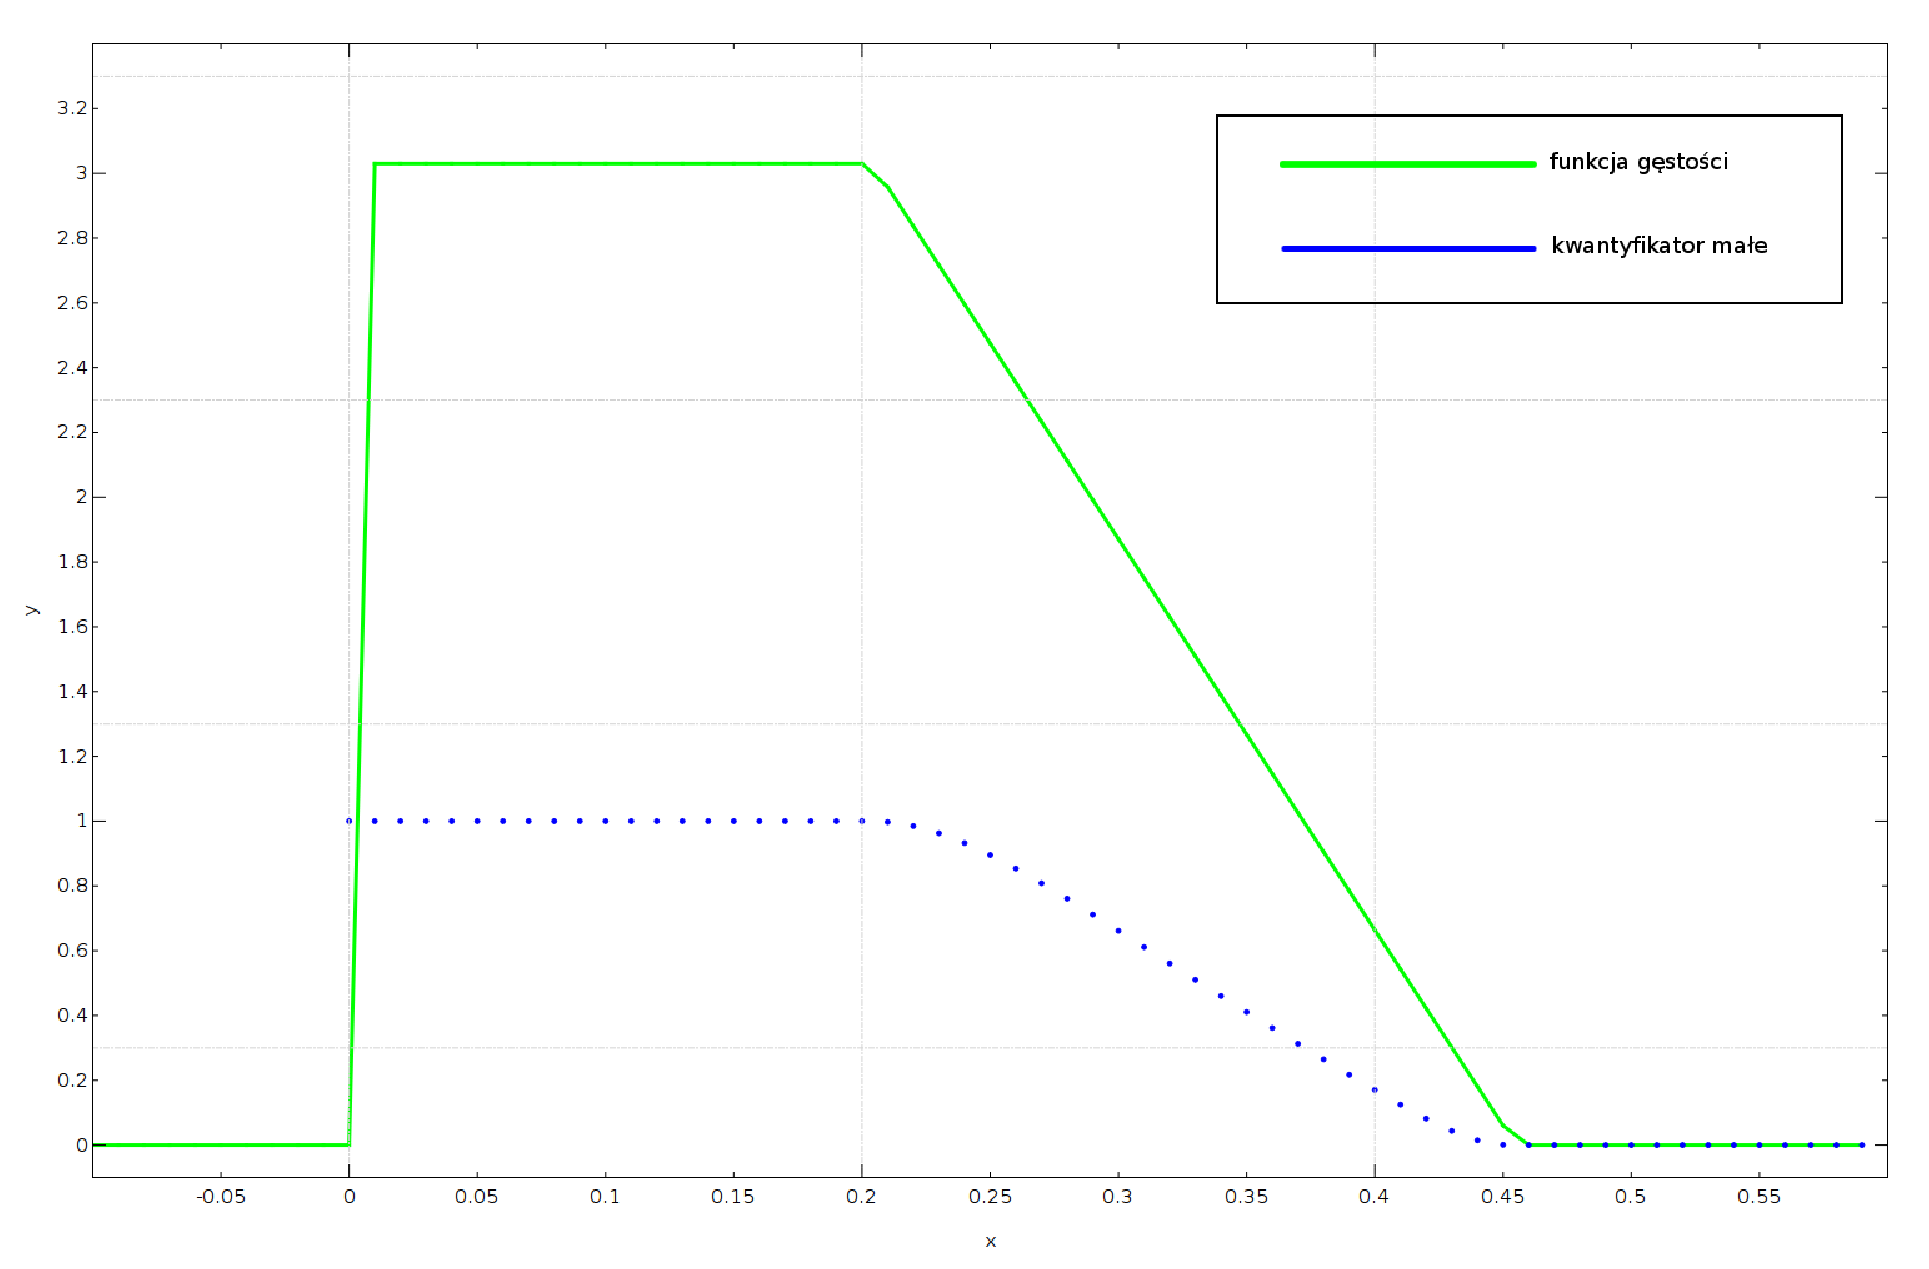
\includegraphics[width=15cm]{male_kwantyfikator_aproksymacja.eps}
      \rule{35em}{0.5pt}
    \caption[Wykres kwantyfikatora \emph{ma�e} wraz z odpowiadaj�c� mu funkcj� rozk�adu g�sto�ci prawdopodobie�stwa]{Wykres kwantyfikatora \emph{ma�e} wraz z funkcj� rozk�adu g�sto�ci prawdopodobie�stwa}
    \label{wykres:male_kwantyfikator_wraz_z_aproksymacja}
\end{figure}
Funkcja rozk�adu g�sto�ci prawdopodobie�stwa, dla kwantyfikatora \emph{du�e}, pokazana na rysunku \ref{wykres:male_kwantyfikator_wraz_z_aproksymacja} wraz z kwantyfikatorem, ma nast�puj�cy wz�r:
\begin{equation}
\label{rownanie:male_wynik}
f(x) = \left\{ 
\begin{array}{l l}
  -8.775*x+3.993, & \quad \text{ dla 0.204 $<$ $x$ $\leq$ 0.454}\\
  2.203, & \quad \text{ dla 0 $<$ $x$ $<$ 0.204}.
\end{array} \right.
\end{equation}
\subsection{Kwantyfikator "bliskie 10 mln"}
Kwantyfikator \emph{bliskie 10 mln} jest zadany przez wykres funkcji \ref{wykres:bliskie10mln}. 
\begin{figure}[ht]
	\centering
	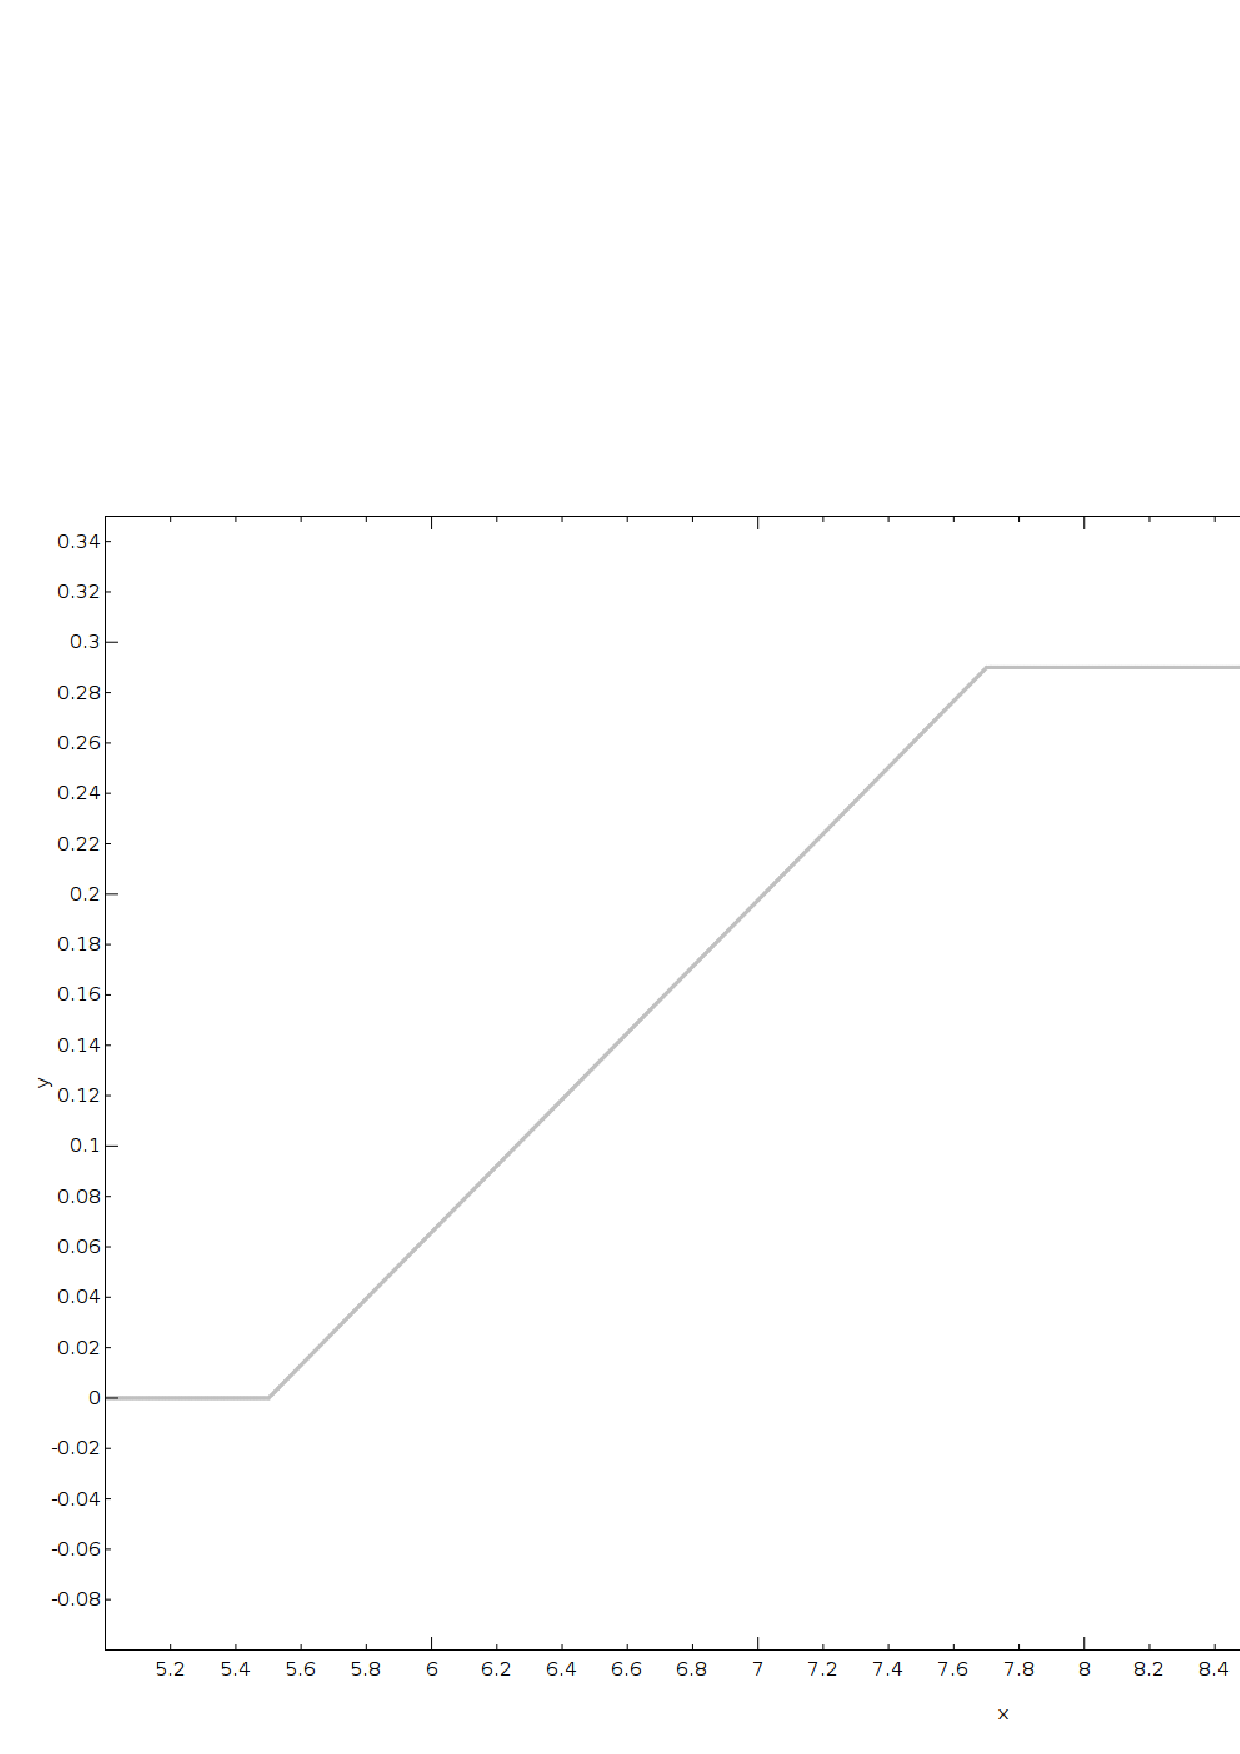
\includegraphics[width=15cm]{bliskie10mln.pdf}
	  \rule{35em}{0.5pt}
	\caption[Wykres funkcji g�sto�ci dla kwantyfikatora  \emph{bliskie 10 mln}]{Wykres funkcji g�sto�ci dla kwantyfikatora  \emph{bliskie 10 mln}}
      \label{wykres:bliskie10mln}
\end{figure}
Tym razem, kwantyfikator ten nie jest wynikiem ankiety, tylko jest zadany przez Profesora Piegata( tak samo jak dla reszty kwantyfikator�w ). 
Aby uzyska� wz�r funkcji dla tego i reszty kwantyfikator�w, rozwi�zujemy uk�ad r�wna� analogiczny do uk�adu \ref{uklad_rownan:duze_ur} o postaci:
\begin{equation}
\label{bliskie10mln_uklad_rownan}
\begin{cases}
(10 - 7.7)*c + \frac{1}{2}*(7.7-5.5)*c = 1\\
5.5*a + b = 0  \\
7.7*a + b = c.
\end{cases}
\end{equation}
Ko�cowa operacja macierzowa wygl�da nast�puj�co:
\begin{equation}
\label{bliskie10mln_mnozenie_macierzy} 
 \begin{bmatrix} 
 a \\ 
 b \\
 c \\
 \end{bmatrix}
 = 
 {\begin{bmatrix} 
 0 & 0 & 3.4 \\ 
 5.5 & 1 & 0 \\
 7.7 & 1 & -1 \\
 \end{bmatrix}}^{-1}
 *
 \begin{bmatrix} 
 1 \\ 
 0 \\
 0 \\
 \end{bmatrix},
\end{equation}
jej rozwi�zaniem jest:
\begin{equation}
 a = 0.13, 
 b = -0.73,  
 c = 0.29.
\end{equation}
Funkcja rozk�adu g�sto�ci prawdopodobie�stwa, kt�ra aproksymuje zbi�r punkt�w danych dla kwantyfikatora  \emph{bliskie 10 mln} przedstawiona zosta�a poni�ej:
\begin{equation}
\label{equation_bliskie10mln_wynik}
f(x) = \left\{ 
\begin{array}{l l}
  0.13*x - 0.73 & \quad \text{, dla 5.5 $<$ $x$ $\leq$ 7.7}\\
  0.29 & \quad \text{, dla 7.7 $<$ $x$ $<$ 1}.
\end{array} \right.
\end{equation}

% 
\subsection{Kwantyfikator "nie bliskie 10 mln"}
Kwantyfikator \emph{nie bliskie 10 mln} jest zadany przez wykres funkcji \ref{wykres:niebliskie10mln}. 
\begin{figure}[ht]
	\centering
	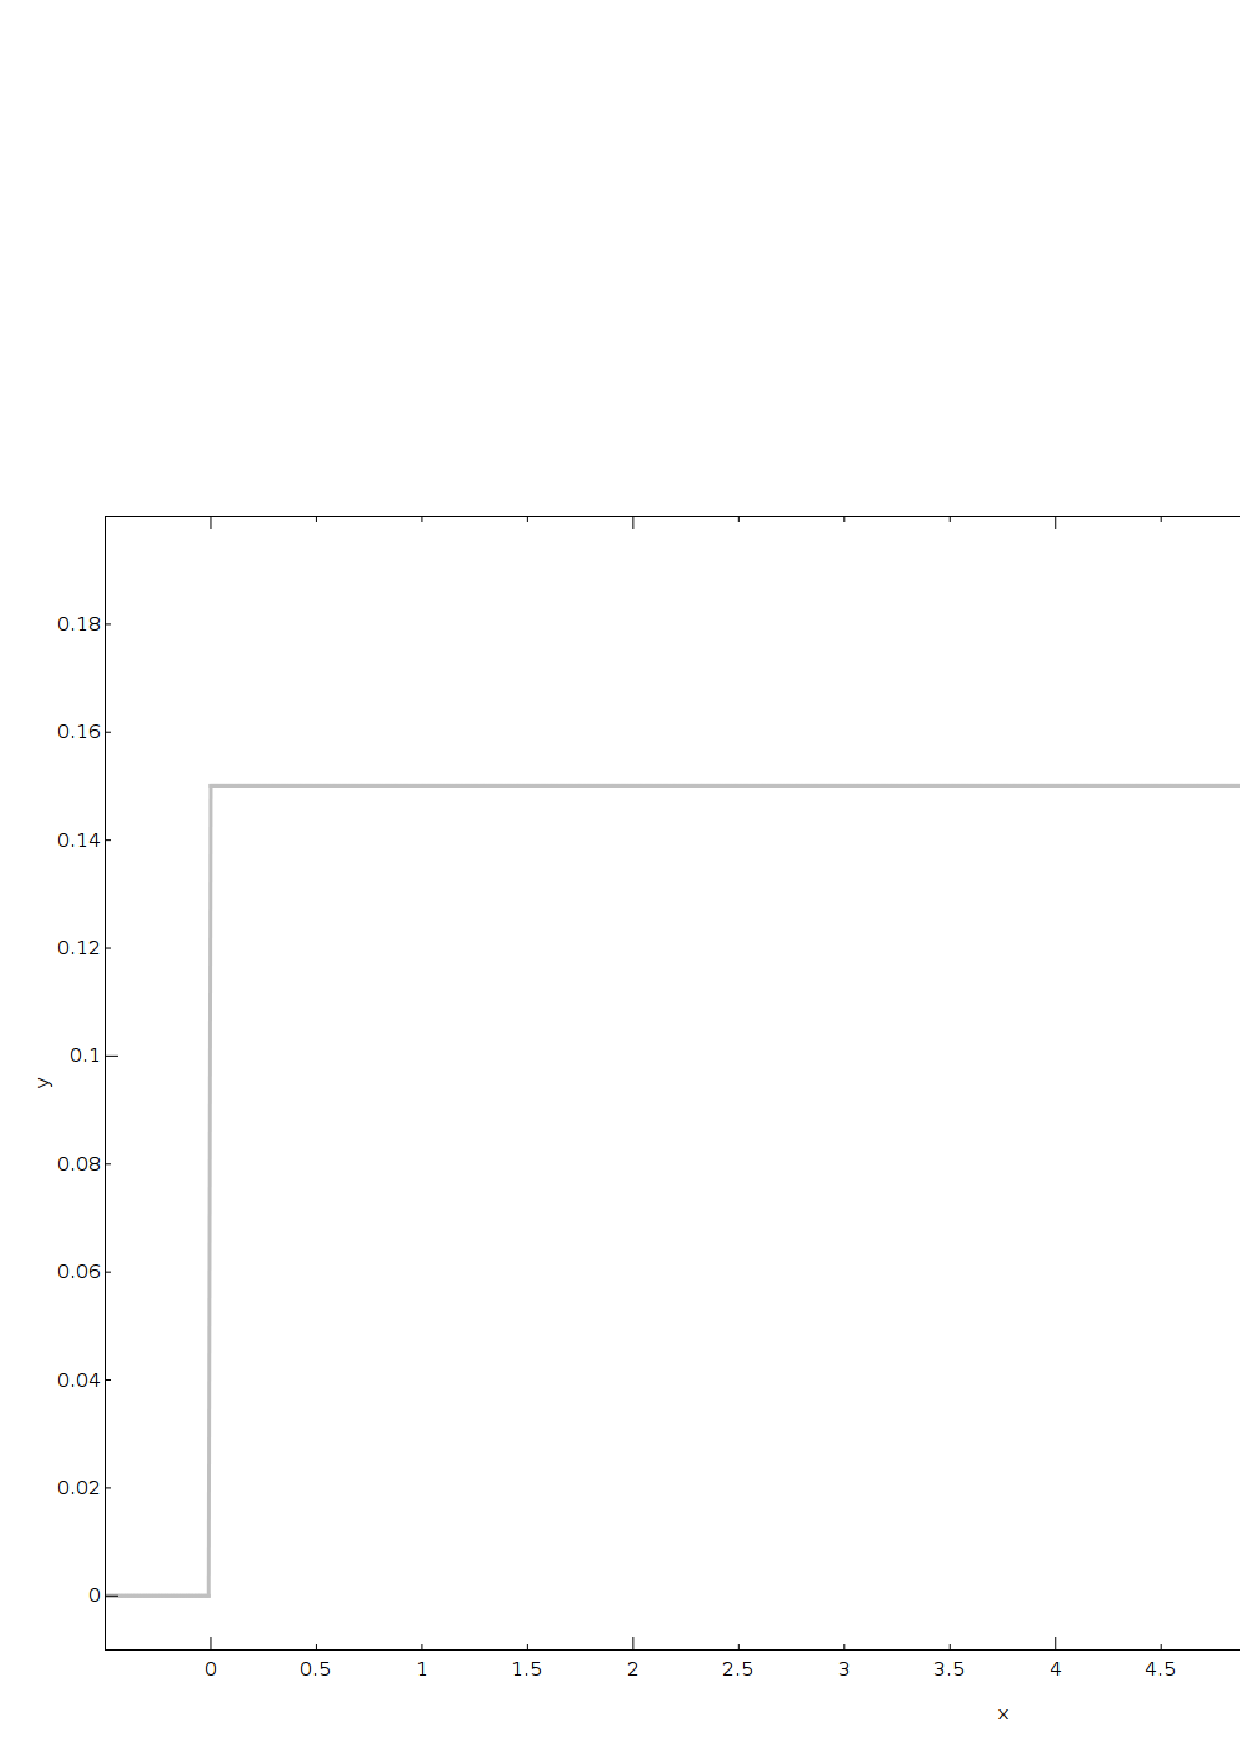
\includegraphics[width=15cm]{niebliskie10mln.pdf}
	  \rule{35em}{0.5pt}
	\caption[Wykres funkcji g�sto�ci dla kwantyfikatora \emph{nie bliskie 10 mln}]{Wykres funkcji g�sto�ci dla kwantyfikatora \emph{nie bliskie 10 mln}}
	\label{wykres:niebliskie10mln}
\end{figure}
Aby uzyska� wz�r funkcji dla tego i reszty kwantyfikator�w, rozwi�zujemy uk�ad r�wna� analogiczny do uk�adu \ref{uklad_rownan:duze_ur} o postaci:
\begin{equation}
\label{niebliskie10mln_uklad_rownan}
\begin{cases}
5.5*c + \frac{1}{2}*(7.7-5.5)*c = 1\\
5.5*a + b = c  \\
7.7*a + b = 0.
\end{cases}
\end{equation}
Finalna operacja macierzowa wygl�da nast�puj�co:
\begin{equation}
\label{niebliskie10mln_mnozenie_macierzy} 
 \begin{bmatrix} 
 a \\ 
 b \\
 c \\
 \end{bmatrix}
 = 
 {\begin{bmatrix} 
 0 & 0 & 6.6 \\ 
 5.5 & 1 & -1 \\
 7.7 & 1 & 0 \\
 \end{bmatrix}}^{-1}
 *
 \begin{bmatrix} 
 1 \\ 
 0 \\
 0 \\
 \end{bmatrix}.
\end{equation}
Rozwi�zanie tego uk�adu jest tr�jka:
\begin{equation}
 a = -0.06, 
 b = 0.53,  
 c = 0.15.
\end{equation}
Funkcja rozk�adu g�sto�ci prawdopodobie�stwa, kt�ra aproksymuje zbi�r punkt�w danych dla kwantyfikatora  \emph{nie bliskie 10 mln} wygl�da zatem nast�puj�co:
\begin{equation}
\label{equation_niebliskie10mln_wynik}
f(x) = \left\{ 
\begin{array}{l l}
 -0.06*x +  0.53, & \quad \text{ dla 5.5 $<$ $x$ $\leq$ 7.7}\\
  0.15, & \quad \text{ dla 0 $<$ $x$ $<$ 5.5}.
\end{array} \right.
\end{equation}.
\subsection{Kwantyfikator "bliskie 20 mln"}
Kwantyfikator \emph{bliskie 20 mln} jest zadany przez wykres funkcji \ref{wykres:bliskie20mln}. 
\begin{figure}[ht]
    \centering
    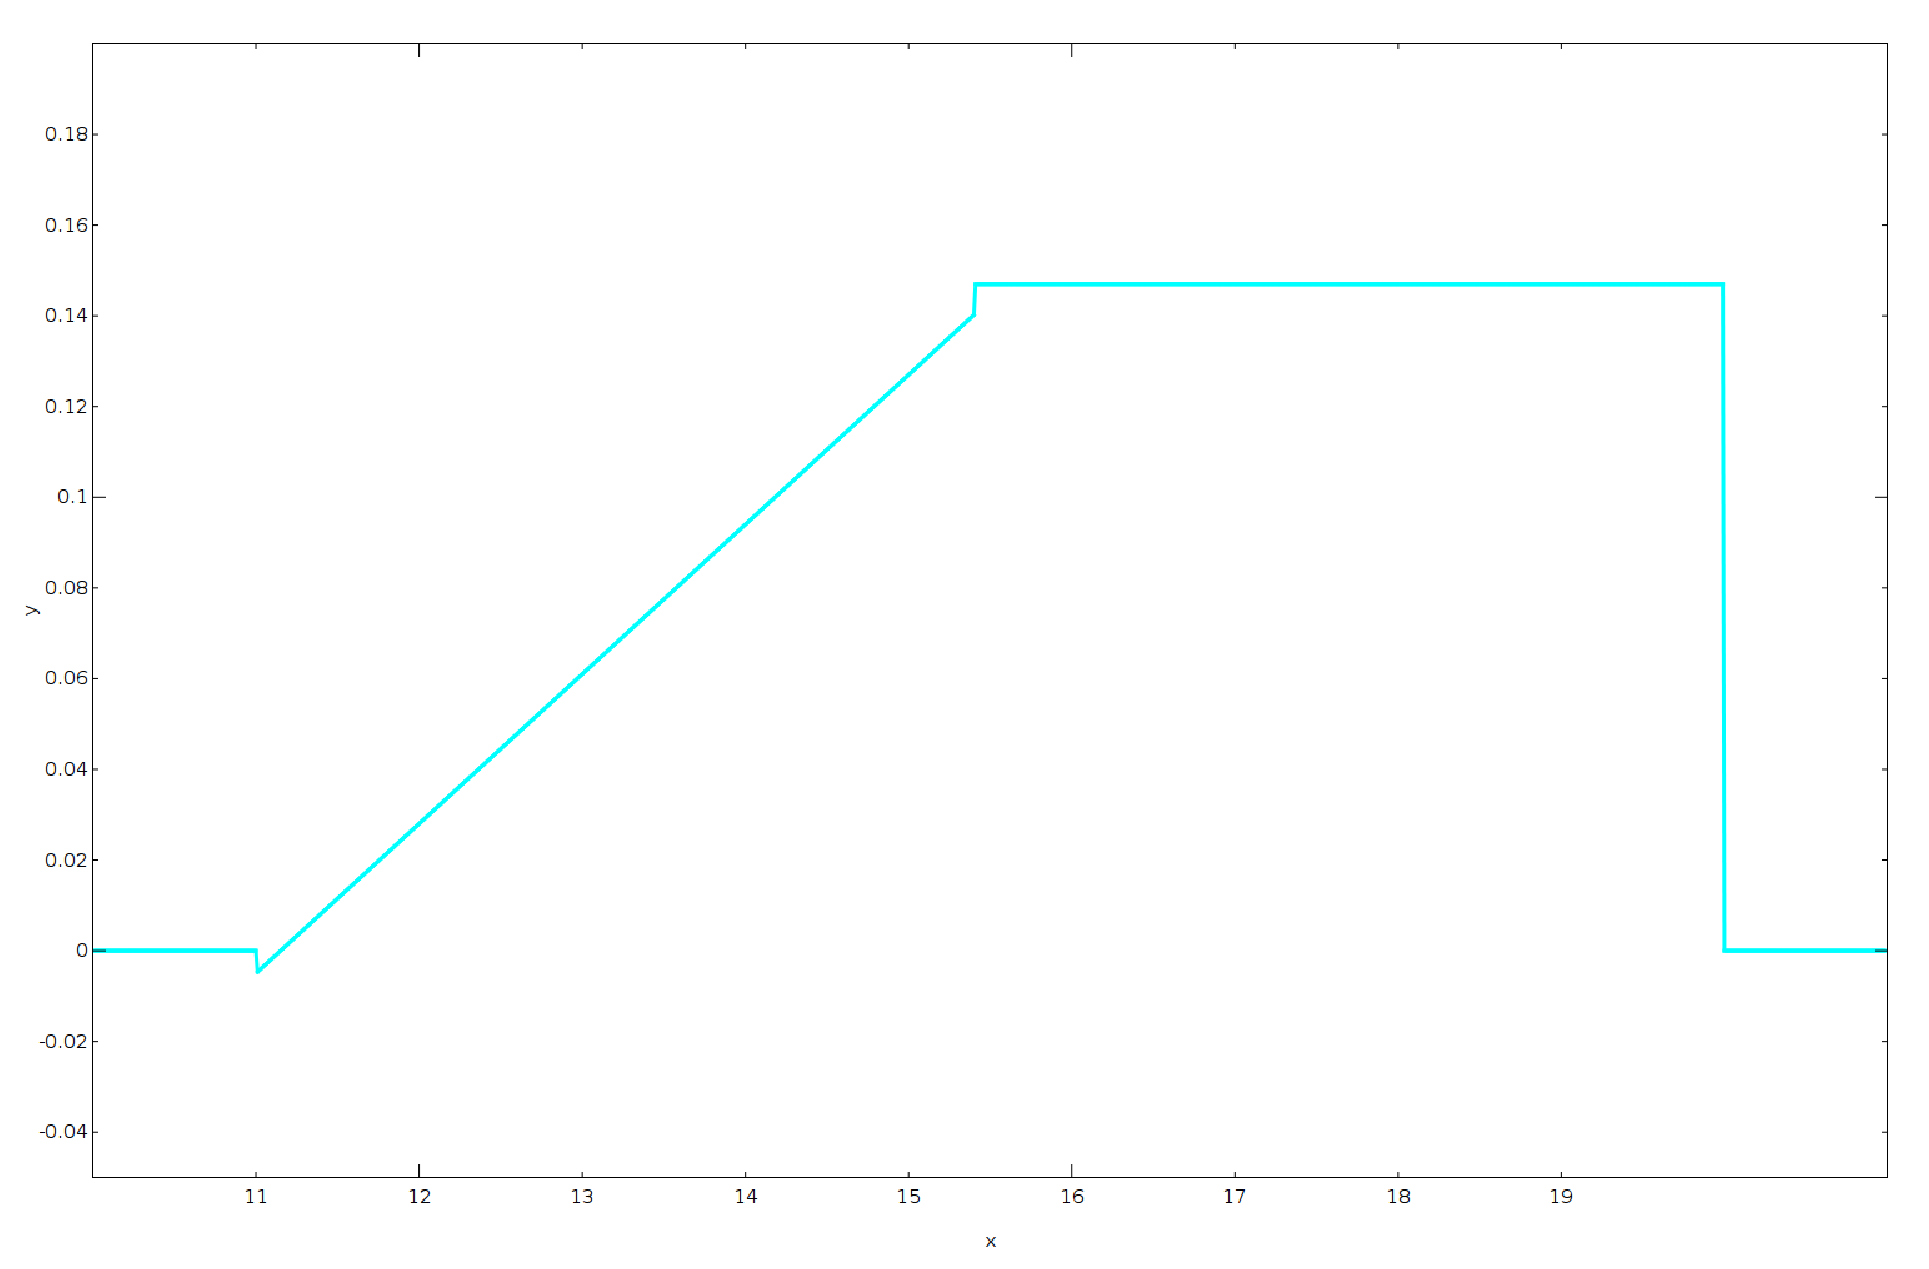
\includegraphics[width=15cm]{bliskie20mln.eps}
        \rule{35em}{0.5pt}
    \caption[Wykres kwantyfikatora bliskie 20 mln]{Wykres funkcji g�sto�ci dla kwantyfikatora \emph{bliskie 20 mln}}
    \label{wykres:bliskie20mln}
\end{figure}
Aby uzyska� wz�r funkcji dla tej funkcji g�sto�ci, rozwi�zujemy uk�ad r�wna� analogiczny do uk�adu \ref{uklad_rownan:duze_ur} o postaci:
\begin{equation}
\label{bliskie20mln_uklad_rownan}
\begin{cases}
(20-15.4)*c + \frac{1}{2}*(15.4-11)*c = 1\\
11*a + b = 0  \\
15.4*a + b = c \\
\end{cases}
\end{equation}.
Finalna operacja macierzowa wygl�da nast�puj�co:
\begin{equation}
\label{bliskie20_mnozenie_macierzy} 
 \begin{bmatrix} 
 a \\ 
 b \\
 c \\
 \end{bmatrix}
 = 
 {\begin{bmatrix} 
 0 & 0 & 6.8 \\ 
 11 & 1 & 0 \\
 15.4 & 1 & -1 \\
 \end{bmatrix}}^{-1}
 *
 \begin{bmatrix} 
 1 \\ 
 0 \\
 0 \\
 \end{bmatrix},
\end{equation}
rozwi�zaniem jest tr�jka:
\begin{equation}
 a = 0.033, 
 b = -0.368,  
 c = 0.147.
\end{equation} 
Funkcja rozk�adu g�sto�ci prawdopodobie�stwa, kt�ra aproksymuje zbi�r punkt�w danych dla kwantyfikatora  \emph{bliskie 20 mln} wygl�da zatem nast�puj�co:
\begin{equation}
\label{equation_bliskie20mln_wynik}
f(x) = \left\{ 
\begin{array}{l l}
 0.02*x -  0.22, & \quad \text{ dla 11 $<$ $x$ $\leq$ 15.4}\\
  0.09, & \quad \text{ dla 15.4 $<$ $x$ $<$ 20} . 
\end{array} \right.
\end{equation}.

\subsection{Kwantyfikator "nie bliskie 20 mln"}
Kwantyfikator \emph{nie bliskie 20 mln} jest zadany przez wykres funkcji \ref{wykres:niebliskie20mln}. 
\begin{figure}[ht]
    \centering
    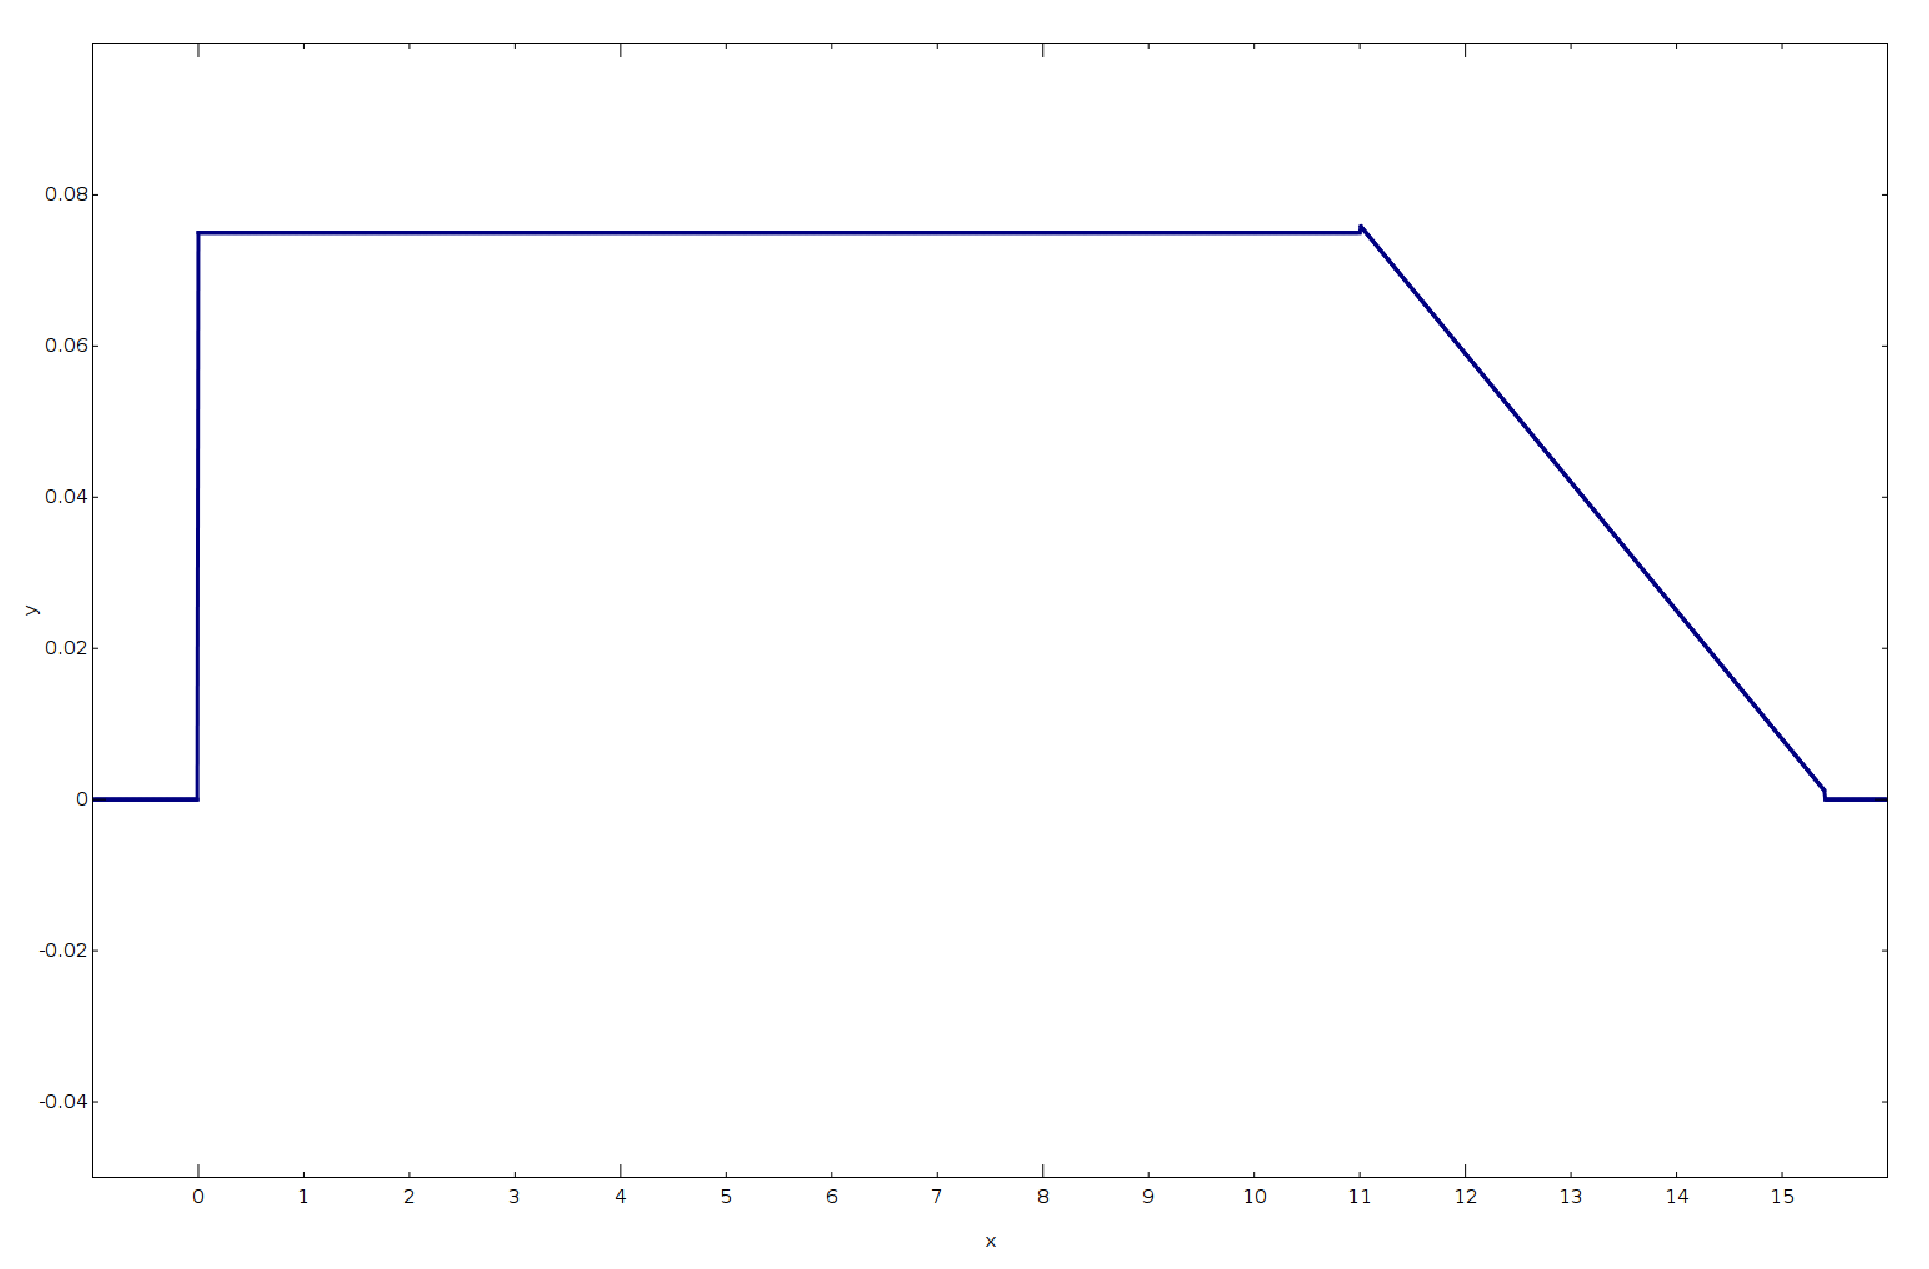
\includegraphics[width=15cm]{niebliskie20mln.eps}
        \rule{35em}{0.5pt}
    \caption[Wykres kwantyfikatora \emph{nie bliskie 20 mln}]{Wykres funkcji g�sto�ci dla kwantyfikatora \emph{nie bliskie 20 mln}}
    \label{wykres:niebliskie20mln}
\end{figure}
Aby uzyska� wz�r funkcji dla tego kwantyfikatora, rozwi�zujemy uk�ad r�wna� analogiczny do uk�adu \ref{uklad_rownan:duze_ur} o postaci:
\begin{equation}
\label{niebliskie20mln_uklad_rownan}
\begin{cases}
11*c + \frac{1}{2}*(15.4-11)*c = 1\\
11*a + b = c  \\
15.4*a + b = 0 .
\end{cases}
\end{equation}
Finalna operacja macierzowa:
\begin{equation}
\label{niebliskie20_mnozenie_macierzy} 
 \begin{bmatrix} 
 a \\ 
 b \\
 c \\
 \end{bmatrix}
 = 
 {\begin{bmatrix} 
 0 & 0 & 13.2 \\ 
 11 & 1 & -1 \\
 15.4 & 1 & 0 \\
 \end{bmatrix}}^{-1}
 *
 \begin{bmatrix} 
 1 \\ 
 0 \\
 0 \\
 \end{bmatrix},
\end{equation}
oraz jej rozwi�zanie
\begin{equation}
 a = -0.017
 b = 0.263,  
 c = 0.075.
\end{equation} 
Funkcja rozk�adu g�sto�ci prawdopodobie�stwa, kt�ra aproksymuje zbi�r punkt�w danych dla kwantyfikatora  \emph{nie bliskie 20 mln} wygl�da zatem nast�puj�co:
\begin{equation}
\label{equation_niebliskie20mln_wynik}
f(x) = \left\{ 
\begin{array}{l l}
 -0.017*x + 0.263, & \quad \text{ dla 11 $<$ $x$ $\leq$ 15.4}\\
  0.075, & \quad \text{ dla 0 $<$ $x$ $<$ 11}.
\end{array} \right.
\end{equation}
Poni�ej, pokazano parami, funkcje rozk�adu g�sto�ci prawdopodobie�stwa dla przeciwstawnych kwantyfikator�w. 
Funkcj� rozk�adu g�sto�ci prawdopodobie�stwa dla kwantyfikator�w \emph{du�e} \emph{ma�e} pokazano na wykresie \ref{wykres:duze_i_male}, dla kwantyfikator�w \emph{bliskie 10 mln} i \emph{nie bliskie 10 mln}, pokazano na wykresie \ref{wykres:kwantyfikatory10mln} a dla kwantyfikator�w \emph{bliskie 20 mln } i \emph{nie bliskie 20 mln } na wykresie \ref{wykres:kwantyfikatory20mln}. 
\begin{figure}[ht]  
    \centering
    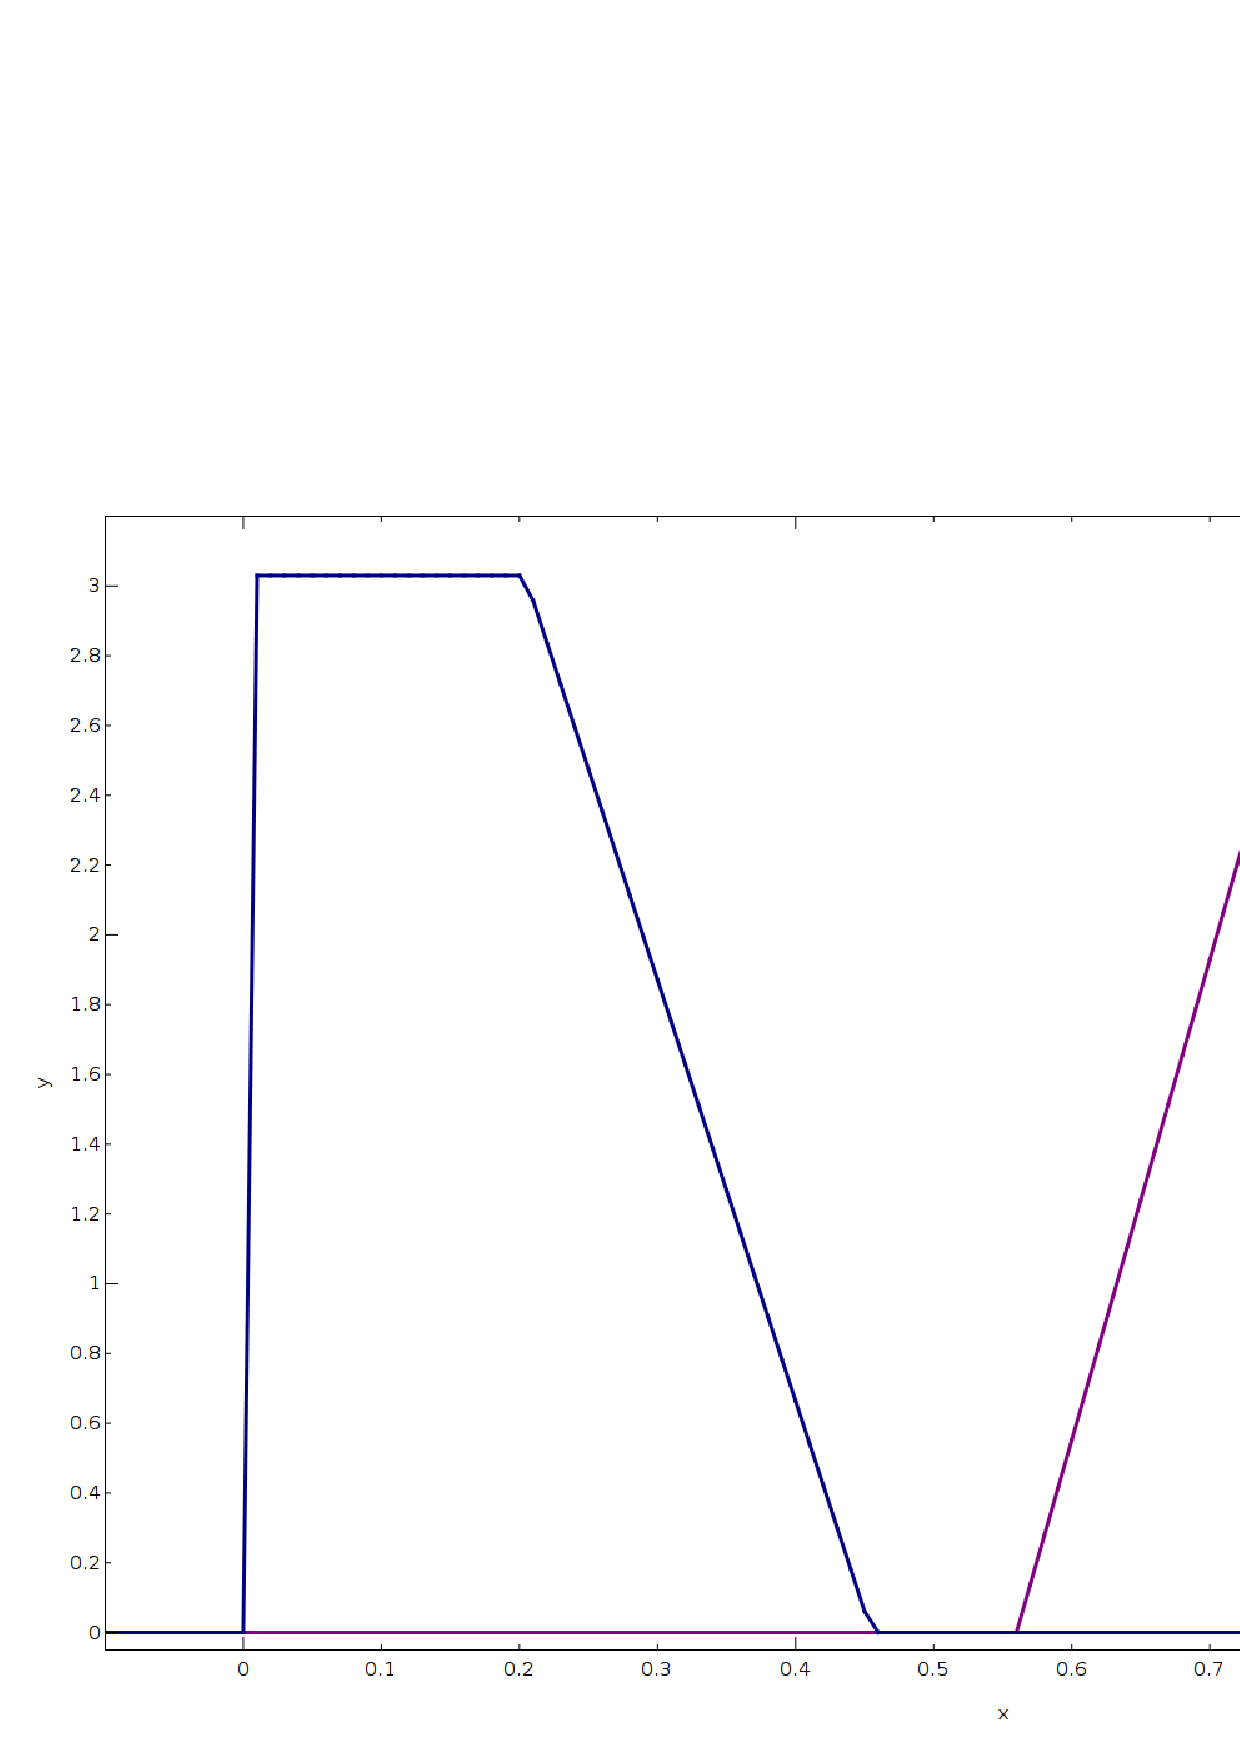
\includegraphics[width=16cm]{male_duze.pdf}
        \rule{35em}{0.5pt}
    \caption[Wykres funkcji g�sto�ci dla kwantyfikator�w \emph{du�e} i \emph{ma�e} ]{Wykres funkcji g�sto�ci dla kwantyfikator�w \emph{du�e} i \emph{ma�e}}
    \label{wykres:duze_i_male}
\end{figure}
\begin{figure}[ht]  
    \centering
    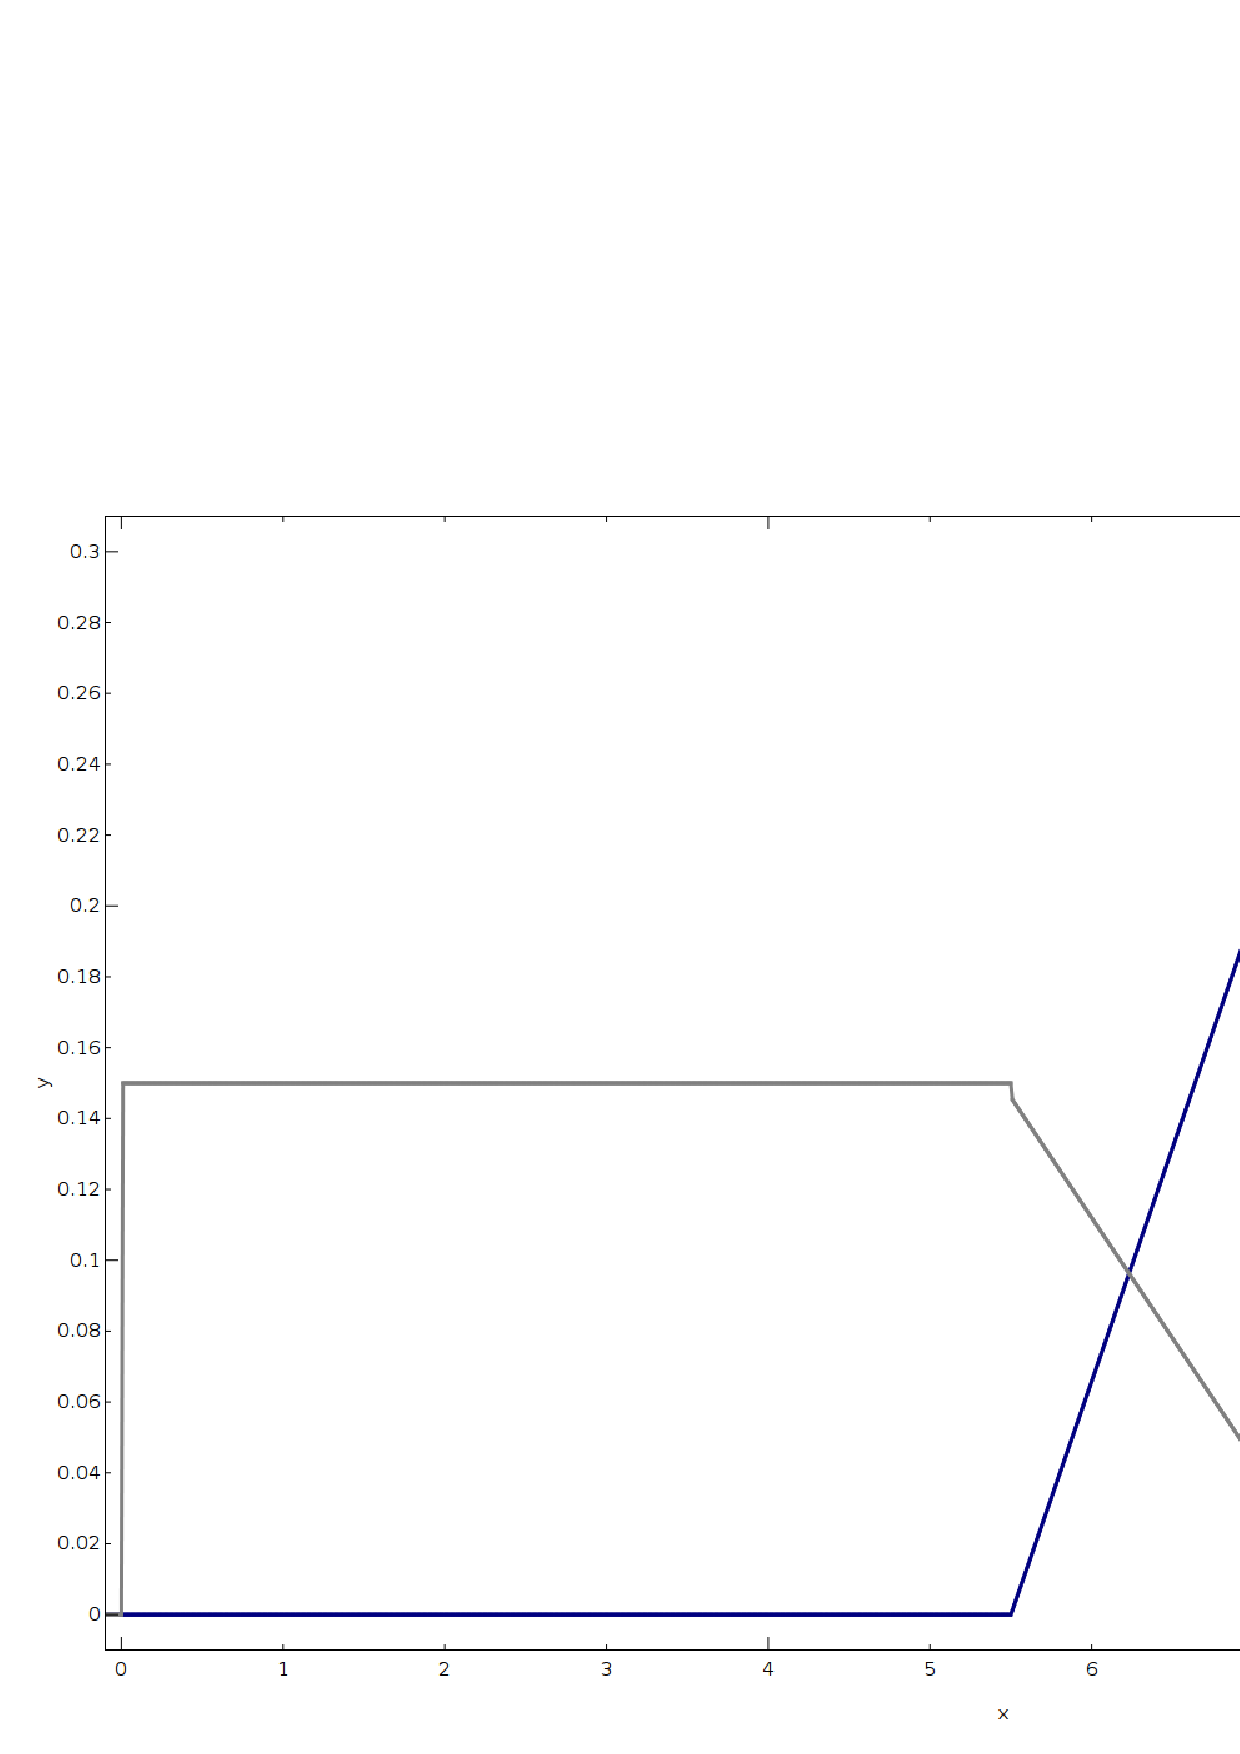
\includegraphics[width=16cm]{kw10mln.pdf}
        \rule{35em}{0.5pt}
    \caption[Wykres funkcji g�sto�ci dla kwantyfikator�w \emph{bliskie 10 mln} i \emph{nie bliskie 10 mln}]{Wykres funkcji g�sto�ci dla kwantyfikator�w \emph{bliskie 10 mln} i \emph{nie bliskie 10 mln}}
    \label{wykres:kwantyfikatory10mln}
\end{figure}
\begin{figure}[ht]  
    \centering
    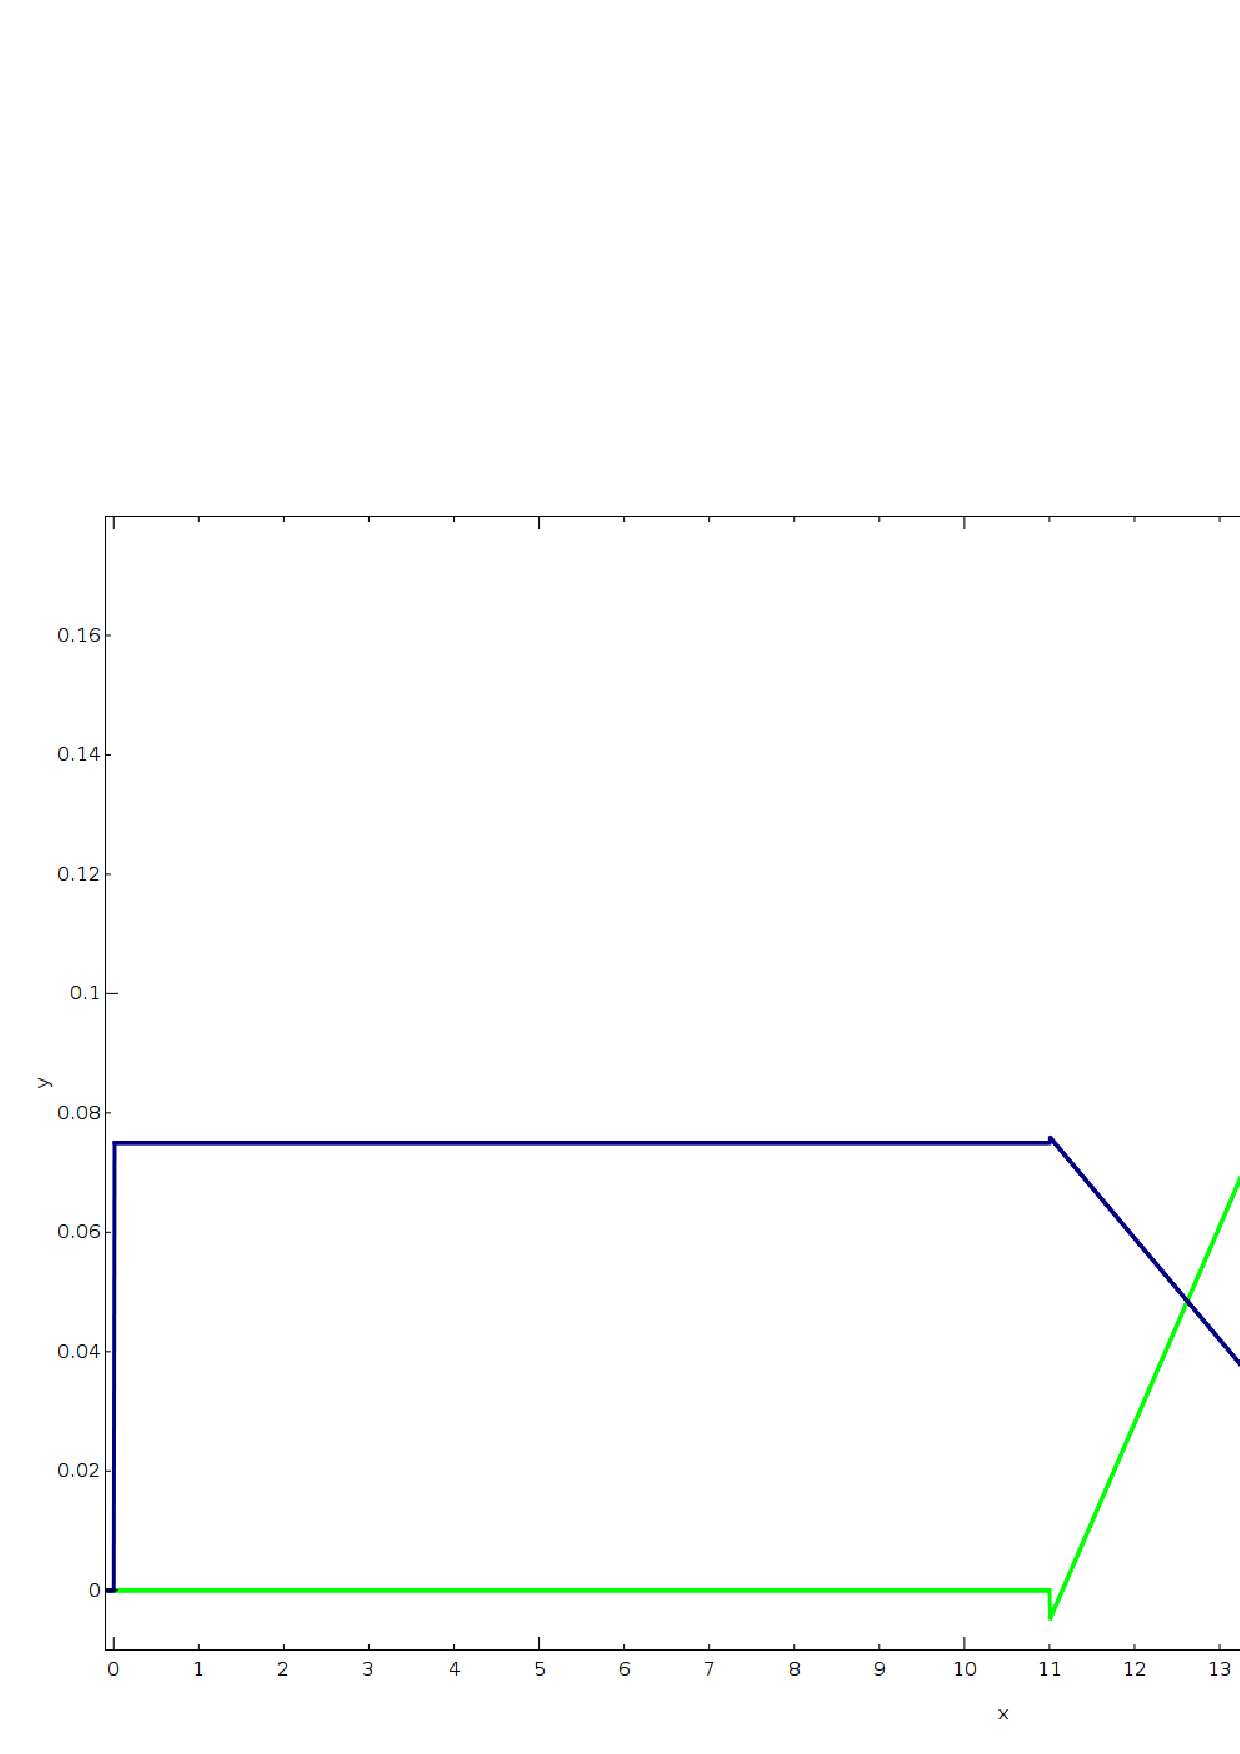
\includegraphics[width=16cm]{kw20mln.pdf}
        \rule{35em}{0.5pt}
    \caption[Wykres funkcji g�sto�ci dla kwantyfikator�w \emph{bliskie 20 mln } i \emph{nie bliskie 20 mln }]{Wykres funkcji g�sto�ci dla kwantyfikator�w \emph{bliskie 20 mln } i \emph{nie bliskie 20 mln }}
    \label{wykres:kwantyfikatory20mln}
\end{figure}
\section{Rozwi�zanie problemu}
Po identyfikacji funkcji rozk�adu g�sto�ci prawdopodobie�stwa, mo�na przyst�pi� do rozwi�zania zadanego problemu. Jako odpowied� na postawiony w zadaniu problem decyzyjny postaramy si� poda� rozk�ady g�sto�ci prawdopodobie�stwa dla biznesu pierwszego oraz biznesu drugiego, oraz policzy� warto�� oczekiwan� z wynikowych rozk�ad�w. Warto�� oczekiwana oraz odchylenie standardowe z tych rozk�ad�w b�d� stanowi�y dla nas podstaw� do ostatecznego podj�cia decyzji, kt�ry biznes, ze statystycznego punktu widzenia, jest bardziej korzystny. 
\subsection{Przedstawienie analitycznej formy rozk�ad�w g�sto�ci prawdopodobie�stwa dla zadania}
Og�lna funkcja rozk�adu g�sto�ci przyjmuje posta�:
\begin{equation}
\label{equation:ogolna_postac_gestosci_rozkladu_prawdopodobienstwa}
gp_{DBn} = f(DBn,p),
\end{equation}
gdzie
\begin{itemize}
\item $gp_{DBn}$ - oznacza g�sto�� rozk�adu prawdopodobie�stwa dochodu z biznesu n-tego
\item $DBn$ - oznacza doch�d z biznesu n-tego
\item $p$ - oznacza prawdopodobie�stwo
\end{itemize}
Funkcj� rozk�adu g�sto�ci prawdopodobie�stwa dla biznesu pierwszego przedstawia si� nast�puj�co:
\begin{equation}
\label{equation:funkcja_rozkladu_gest_prawd_biznes1}
gp_{DB1} = \newline f(DB1,p) = fb10mln(p)\otimes D(p) \oplus fnb10mln(p)\otimes M(p),
\end{equation}
gdzie 
\begin{itemize}
 \item $fb10mln(p)$ - oznacza funkcj� rozk�adu g�sto�ci dla kwantyfikatora \emph{bliskie 10 mln}
 \item $D(p)$ - oznacza funkcj� rozk�adu g�sto�ci dla kwantyfikatora \emph{du�e}
 \item $fnb10mln(p)$ - oznacza funkcj� rozk�adu g�sto�ci dla kwantyfikatora \emph{nie bliskie 10 mln}
 \item $M(p)$ - oznacza funkcj� rozk�adu g�sto�ci dla kwantyfikatora \emph{ma�e}
\end{itemize}
Analogicznie, by okre�lamy funkcj� rozk�adu g�sto�ci prawdopodobie�stwa dla biznesu drugiego:
\begin{equation}
\label{equation:funkcja_rozkladu_gest_prawd_biznes2}
gp_{DB2} = \newline f(DB1,p) = fb20mln(p)\otimes M(p) \oplus fnb20mln(p)\otimes D(p),
\end{equation}
gdzie 
\begin{itemize}
 \item $fb20mln(p)$ - oznacza funkcj� rozk�adu g�sto�ci dla kwantyfikatora \emph{bliskie 20 mln}
 \item $D(p)$ - oznacza funkcj� rozk�adu g�sto�ci dla kwantyfikatora \emph{du�e}
 \item $fnb20mln(p)$ - oznacza funkcj� rozk�adu g�sto�ci dla kwantyfikatora \emph{nie bliskie 20 mln}
 \item $M(p)$ - oznacza funkcj� rozk�adu g�sto�ci dla kwantyfikatora \emph{ma�e}
\end{itemize}

Gdy uda nam si� ustali� obie funkcje, nale�y policzy� warto�� oczekiwan� takiego rozk�adu oraz odchylenie standardowe, co b�dzie stanowi�o dla nas statystyczn� odpowied�. 
\subsection{Funkcje rozk�adu g�sto�ci prawdopodobie�stwa dla biznesu pierwszego}
Funkcja g�sto�ci rozk�adu prawdopodobie�stwa jest dana wzorem \ref{equation:funkcja_rozkladu_gest_prawd_biznes1}. 
Zanim zostanie przedstawiona ko�cowa funkcje g�sto�ci, pokazane zostan� wyniki posi�kowe poszczeg�lnych operacji. 
Pierwsz� operacj� jest operacja:
\begin{equation}
\label{equation:pierwsza_operacja_biznes1}
biznes1f1(x) = fb10mln(p)\otimes D(p), 
\end{equation}
kt�ra zachodzi mi�dzy funkcjami rozk�ad�w g�sto�ci prawdopodobie�stwa dla kwantyfikator�w \emph{bliskie 10 mln} i \emph{du�e}.Operacja ta $\otimes$ zosta�a opisana w rozdziale 2. Wynik tego dzia�ania zosta� przedstawiony na wykresie \ref{wykres:frgp_biznes1_op1}. Funkcja, kt�ra powstaje w wyniku tej operacji, wyliczona w programie jest funkcj� dyskretn� okre�lon� w danych punktach. Poniewa�, nas interesuj� jedynie funkcje ci�g�e, funkcja ta musi zosta� zaaproksymowana na zadanym przedziale ( pami�tamy o tym �e funkcja b�d�ca wynikiem aproksymacji, r�wnie� musi by� funkcj� g�sto��, co oznacza jej ca�kowalno�� do 1) . Wykres \ref{wykres:frgp_biznes1_op1_aproksymacja} przedstawia funkcj� dyskretn� oraz jej aproksymacj� do wielomianu 6-tego stopnia. Stopnie wielomianu, w tej operacji przybli�enia, oraz w pozosta�ych, zosta�y ustalone empirycznie poprzez minimalizacj� odchylenia odchy�ki funkcji od jej przybli�enia. R�wnanie funkcji zosta�o przedstawione na wzorze\footnote{program podaje du�o dok�adniejsze warto�ci sta�ych w aproksymowanych wielomianach, ale autor zdecydowa� si� podawa� ich zaokr�glon� posta�, w celach estetycznych} \ref{wzor:fgrp1_biznes1_op1_aproks_rownanie}:
\begin{equation}
\label{wzor:fgrp1_biznes1_op1_aproks_rownanie}
biznes1f1(x) = \left\{ 
\begin{array}{l l}
 \frac{-7.2+8.8-4.2x^2 + 1.0x^3-0.1x^6 }{0.98}, & \quad \text{ dla 3.08 $<$ $x$ $\leq$ 9.98}\\
  0, & \quad \text{ dla $-\infty$ $<$ $x$ $<$ 3.08 }\\
  0, & \quad \text{ dla 9.98 $<$ $x$ $<$ $\infty$}\\
\end{array} \right. .
\end{equation}
\begin{figure}[ht]
    \centering
    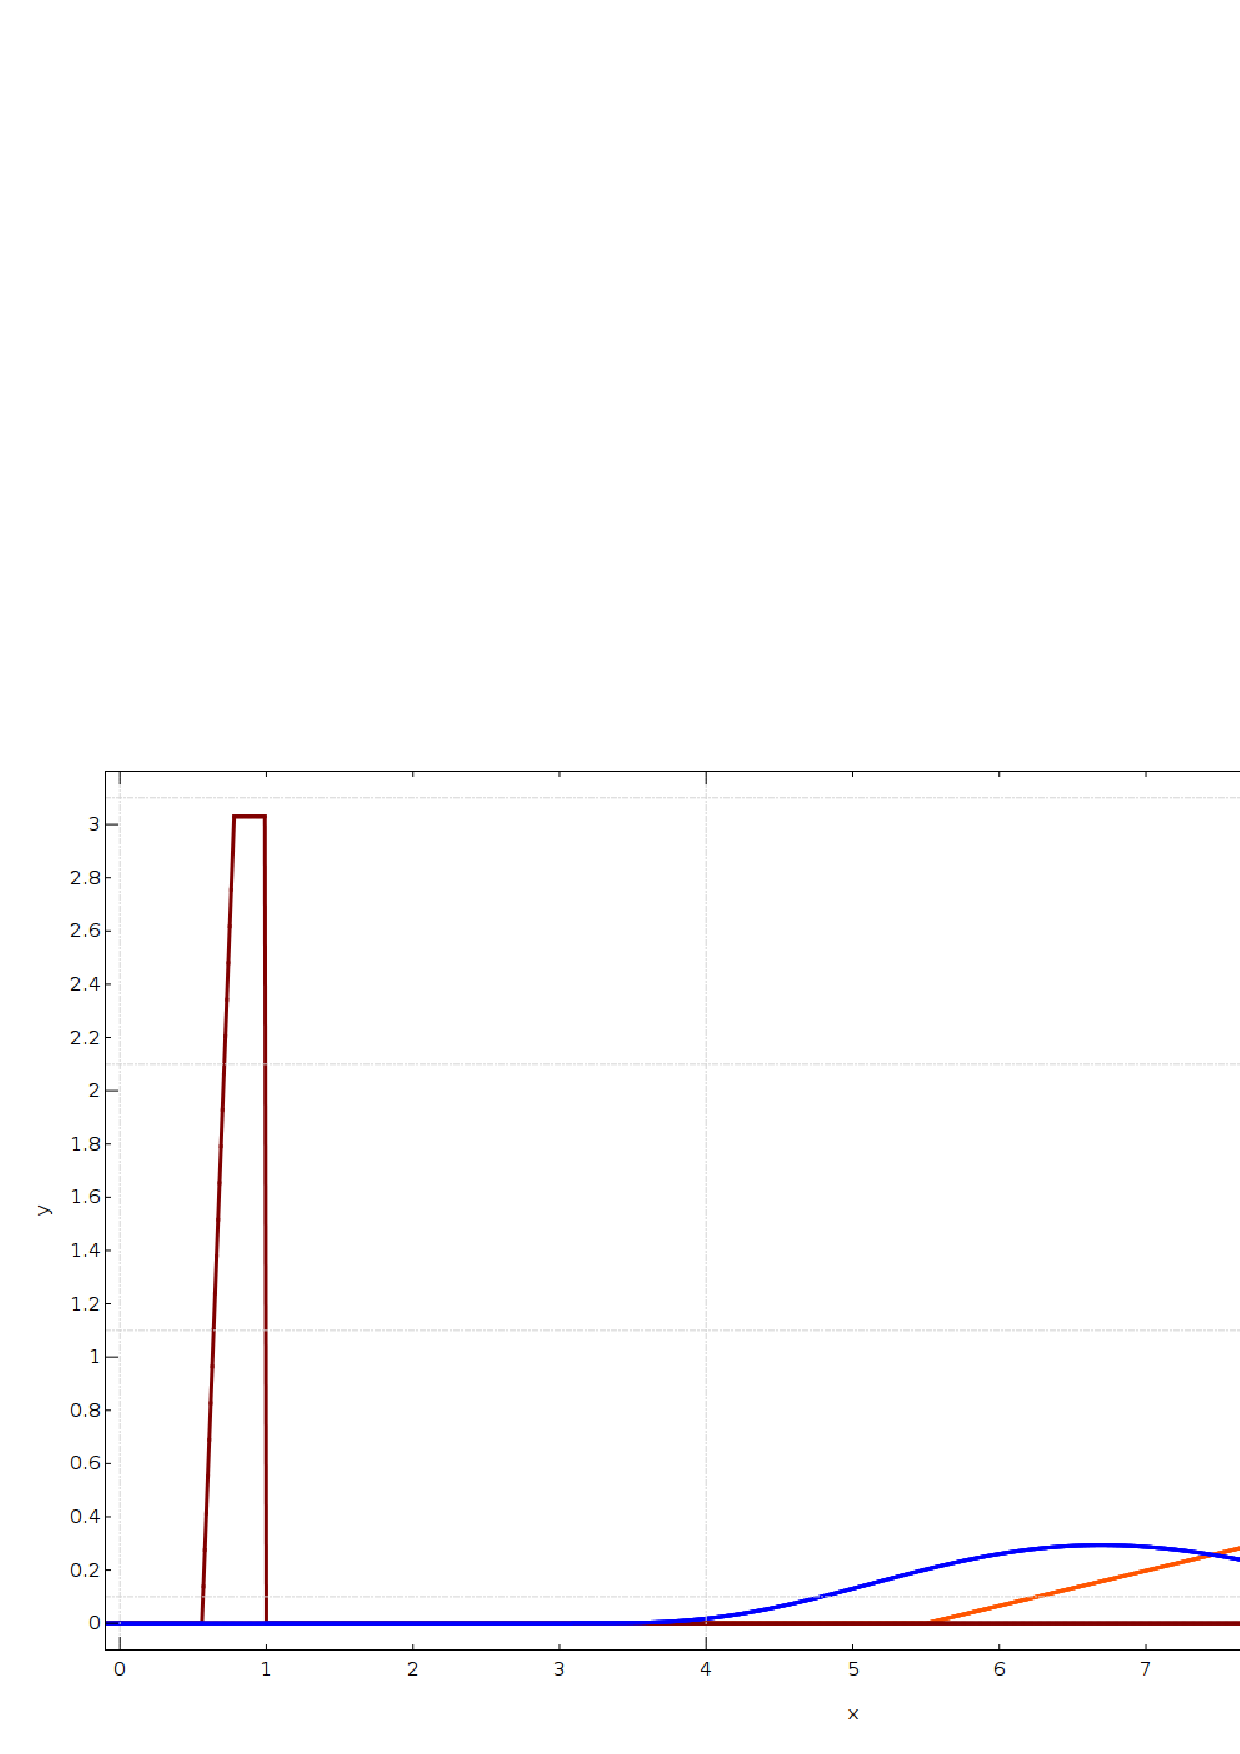
\includegraphics[width=16cm]{frgp_biznes1_op1.pdf}
        \rule{35em}{0.5pt}
    \label{wykres:frgp_biznes1_op1}
\end{figure}

Jak wida� na wykresie \ref{wykres:frgp_biznes1_op1_aproksymacja}, aproksymacja ta jest bardzo dok�adna na przedziale i jej b��d jest niewielki. 
\begin{figure}[ht]  
    \centering
    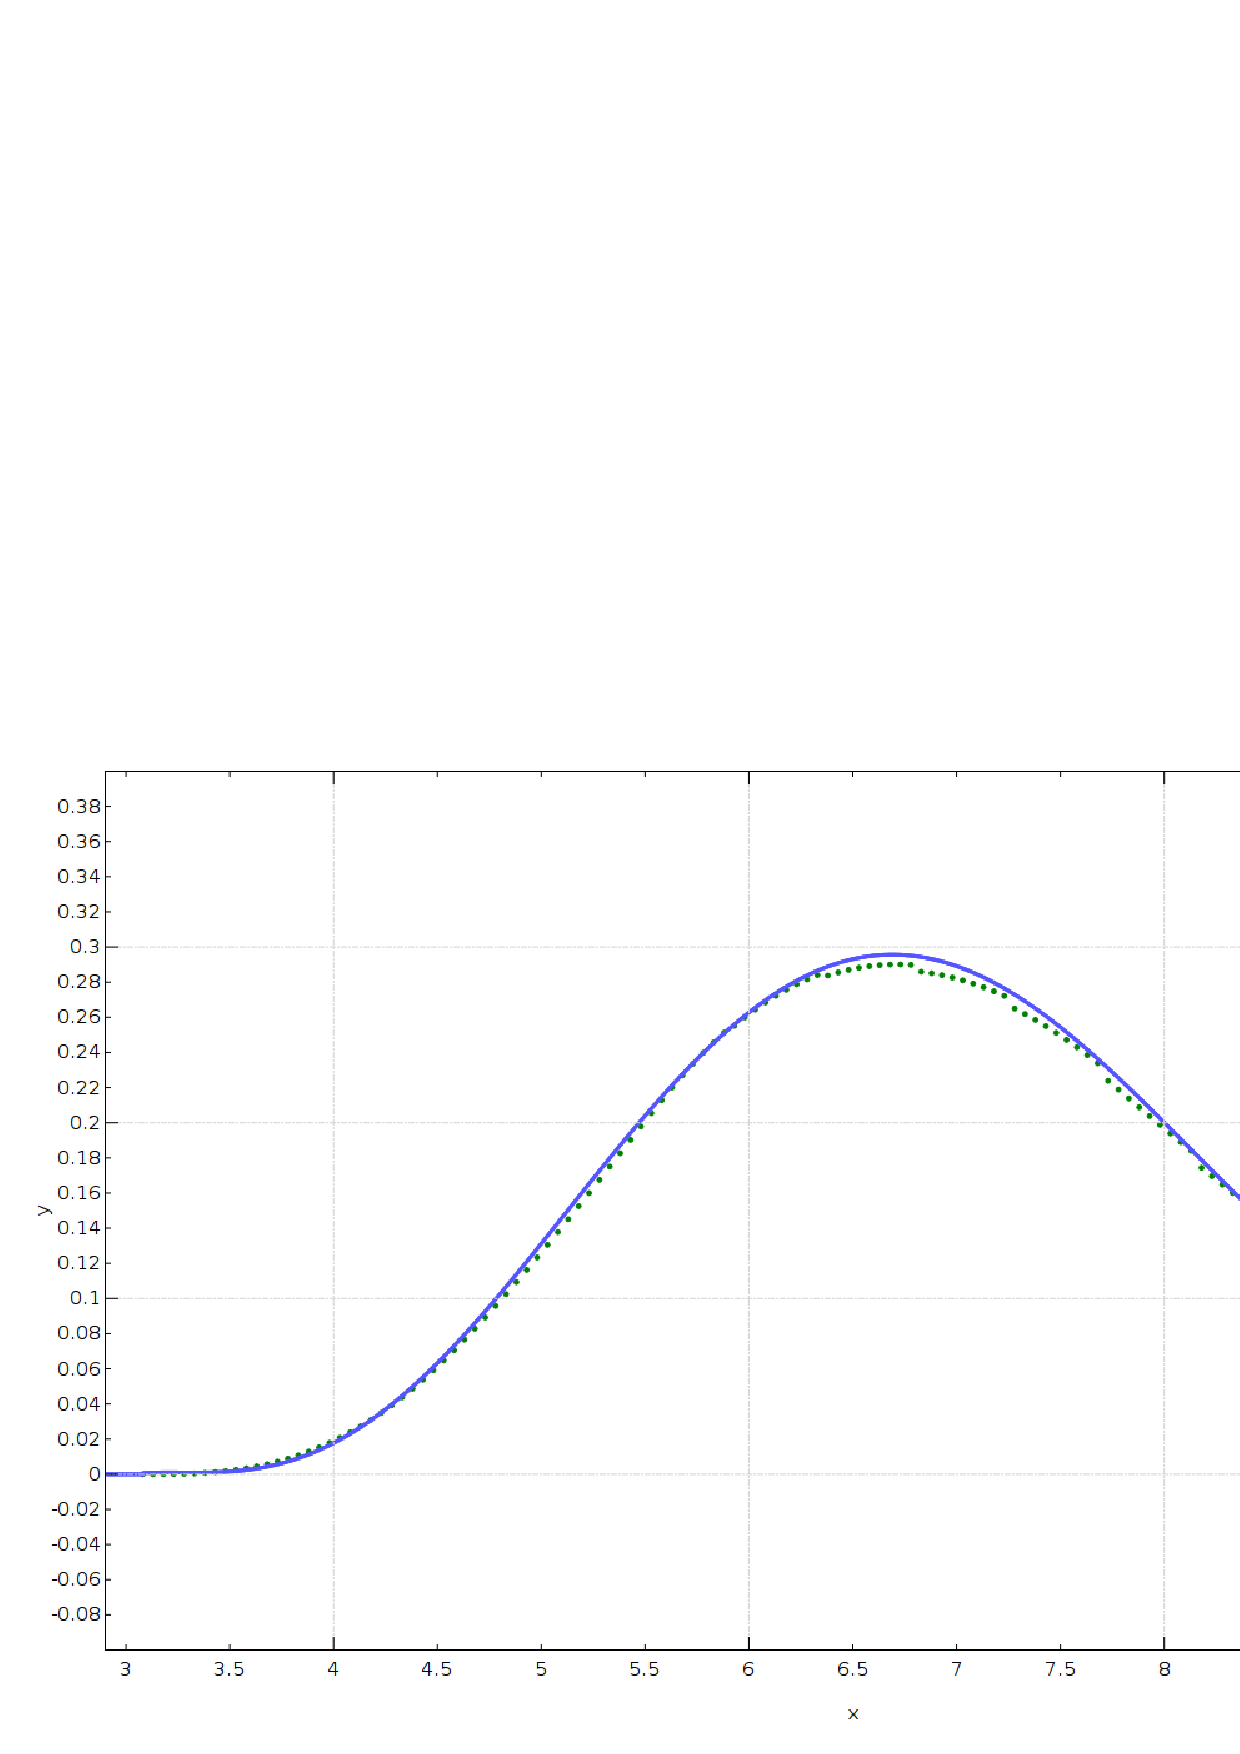
\includegraphics[width=16cm]{frgp_biznes1_op1_aproksymacja.pdf}
        \rule{35em}{0.5pt}
    \caption[Wykres przedstawiaj�cy niedok�adno�� aproksymacji funkcji g�sto�ci \emph{bliskie 10 mln}$\otimes$\emph{du�e}]{Wykres przedstawiaj�cy niedok�adno�� aproksymacji funkcji g�sto�ci \emph{bliskie 10 mln}$\otimes$ \emph{du�e}}
    \label{wykres:frgp_biznes1_op1_aproksymacja}
\end{figure}
\newline
Nast�pnym dzia�aniem jest:
\begin{equation}
\label{equation:druga_operacja_biznes1}
biznes1f2(x) = fnb10mln(p)\otimes M(p).
\end{equation}
Wynik tej operacji zosta� przedstawiony na wykresie \ref{wykres:frgp_biznes1_op2}. Tak jak w przypadku operacji \ref{equation:pierwsza_operacja_biznes1} tak w tym przypadku powsta�a funkcja jest funkcj� dyskretn� wymagaj�c� aproksymacji na przedziale. R�wnanie funkcji zosta�o przedstawione na wzorze \ref{wzor:fgrp1_biznes1_op2_aproks_rownanie}, a niedok�adno�ci aproksymacji na wykresie \ref{wykres:frgp_biznes1_op2_aproksymacja}. 
\begin{figure}[ht]  
    \centering
    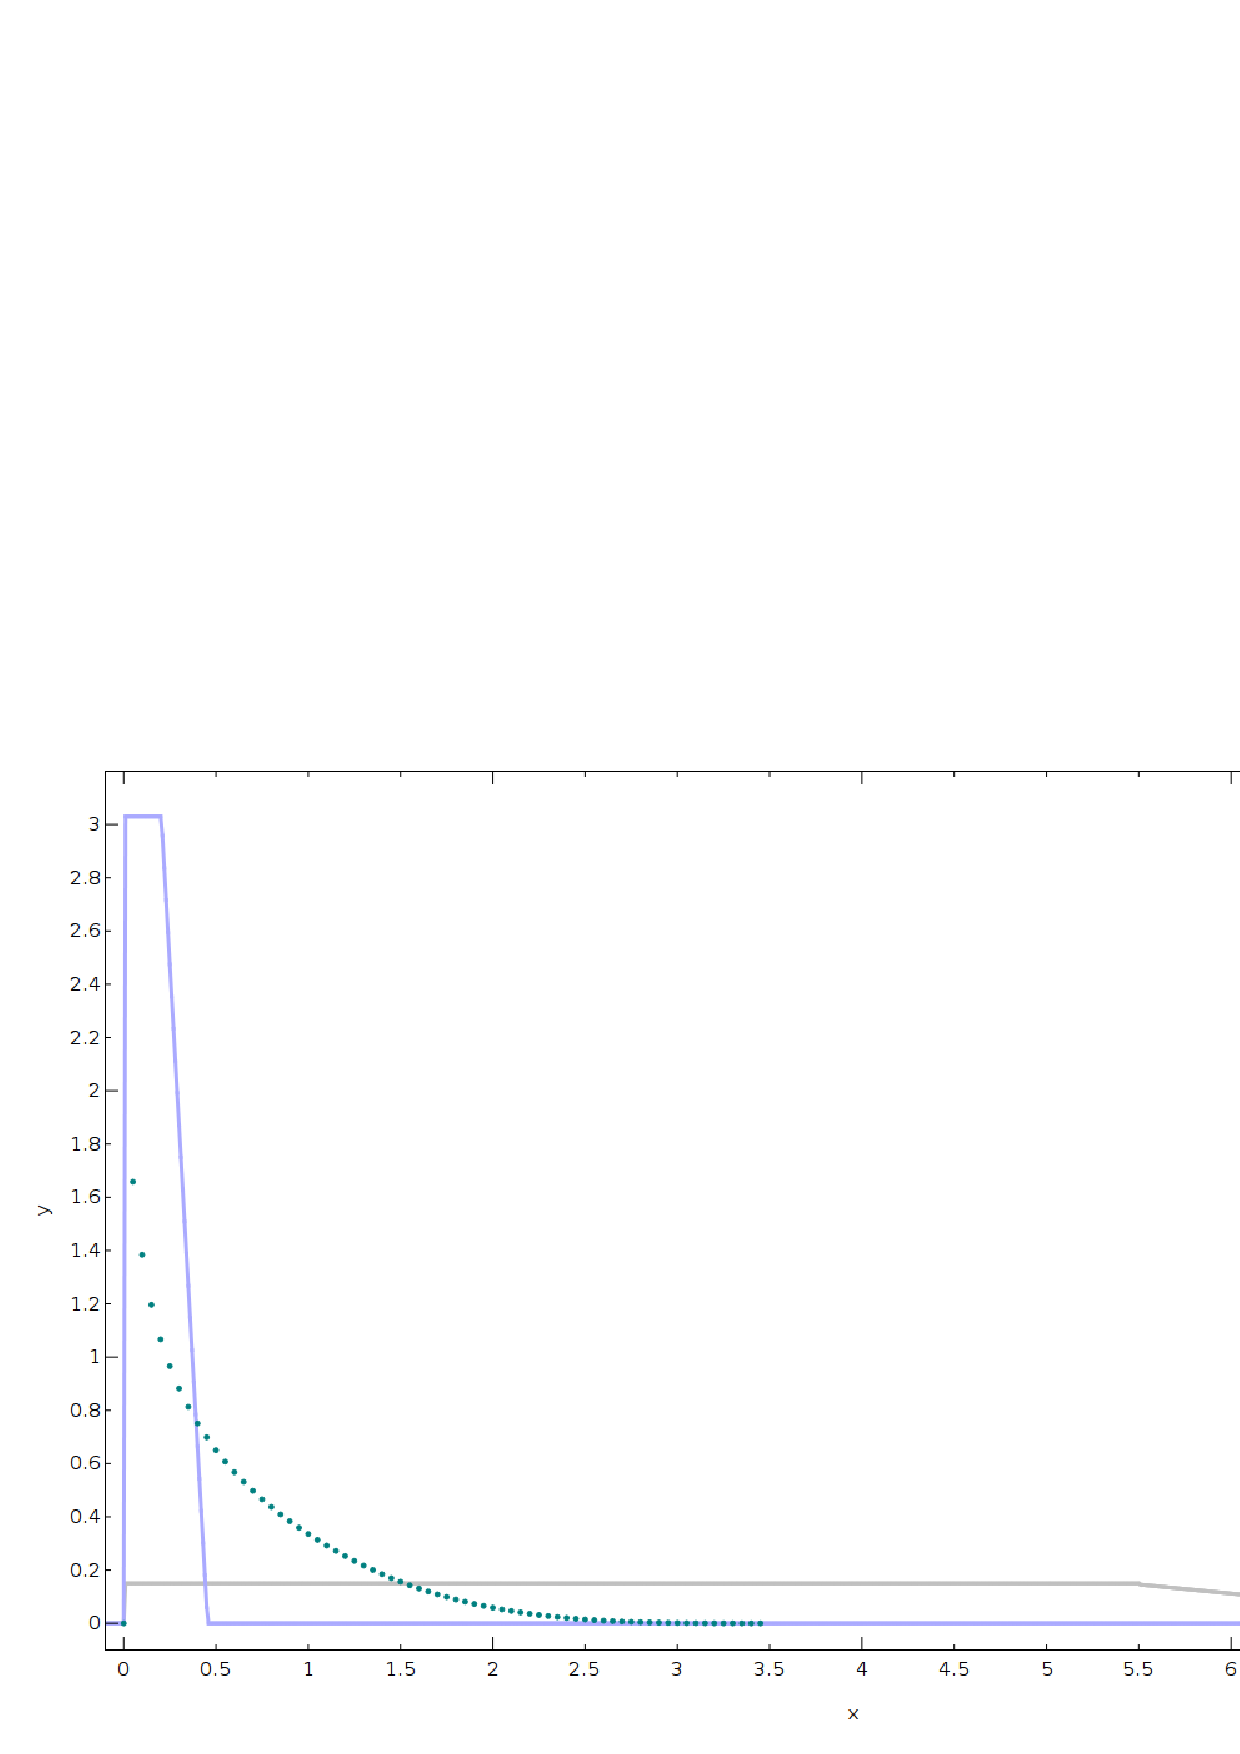
\includegraphics[width=16cm]{frgp_biznes1_op2.pdf}
        \rule{35em}{0.5pt}
    \caption[Wykres funkcji g�sto�ci dla kwantyfikator�w \emph{ma�e} i \emph{nie bliskie 10 mln} oraz funkcji wynikowej dla operacji $\otimes$ mi�dzy nimi]{Wykres funkcji g�sto�ci dla kwantyfikator�w \emph{ma�e} i \emph{nie bliskie 10 mln} oraz funkcji wynikowej dla operacji $\otimes$ mi�dzy nimi}
    \label{wykres:frgp_biznes1_op2}
\end{figure}
\begin{equation}
\label{wzor:fgrp1_biznes1_op2_aproks_rownanie}
biznes1f2(x) = \left\{ 
\begin{array}{l l}
 \frac{2.5-13.4x+40.2x^2-64.1x^3+57.4x^4-30.0x^5+9x^6-1.4x^7+0.09x^8}{0.97}, & \quad \text{ dla 0 $<$ $x$ $\leq$ 3.45}\\
  0, & \quad \text{ dla $-\infty$ $<$ $x$ $<$ 0 }\\
  0, & \quad \text{ dla 3.45 $<$ $x$ $<$ $\infty$}\\
\end{array} \right.
\end{equation}
\begin{figure}[ht]  
    \centering
    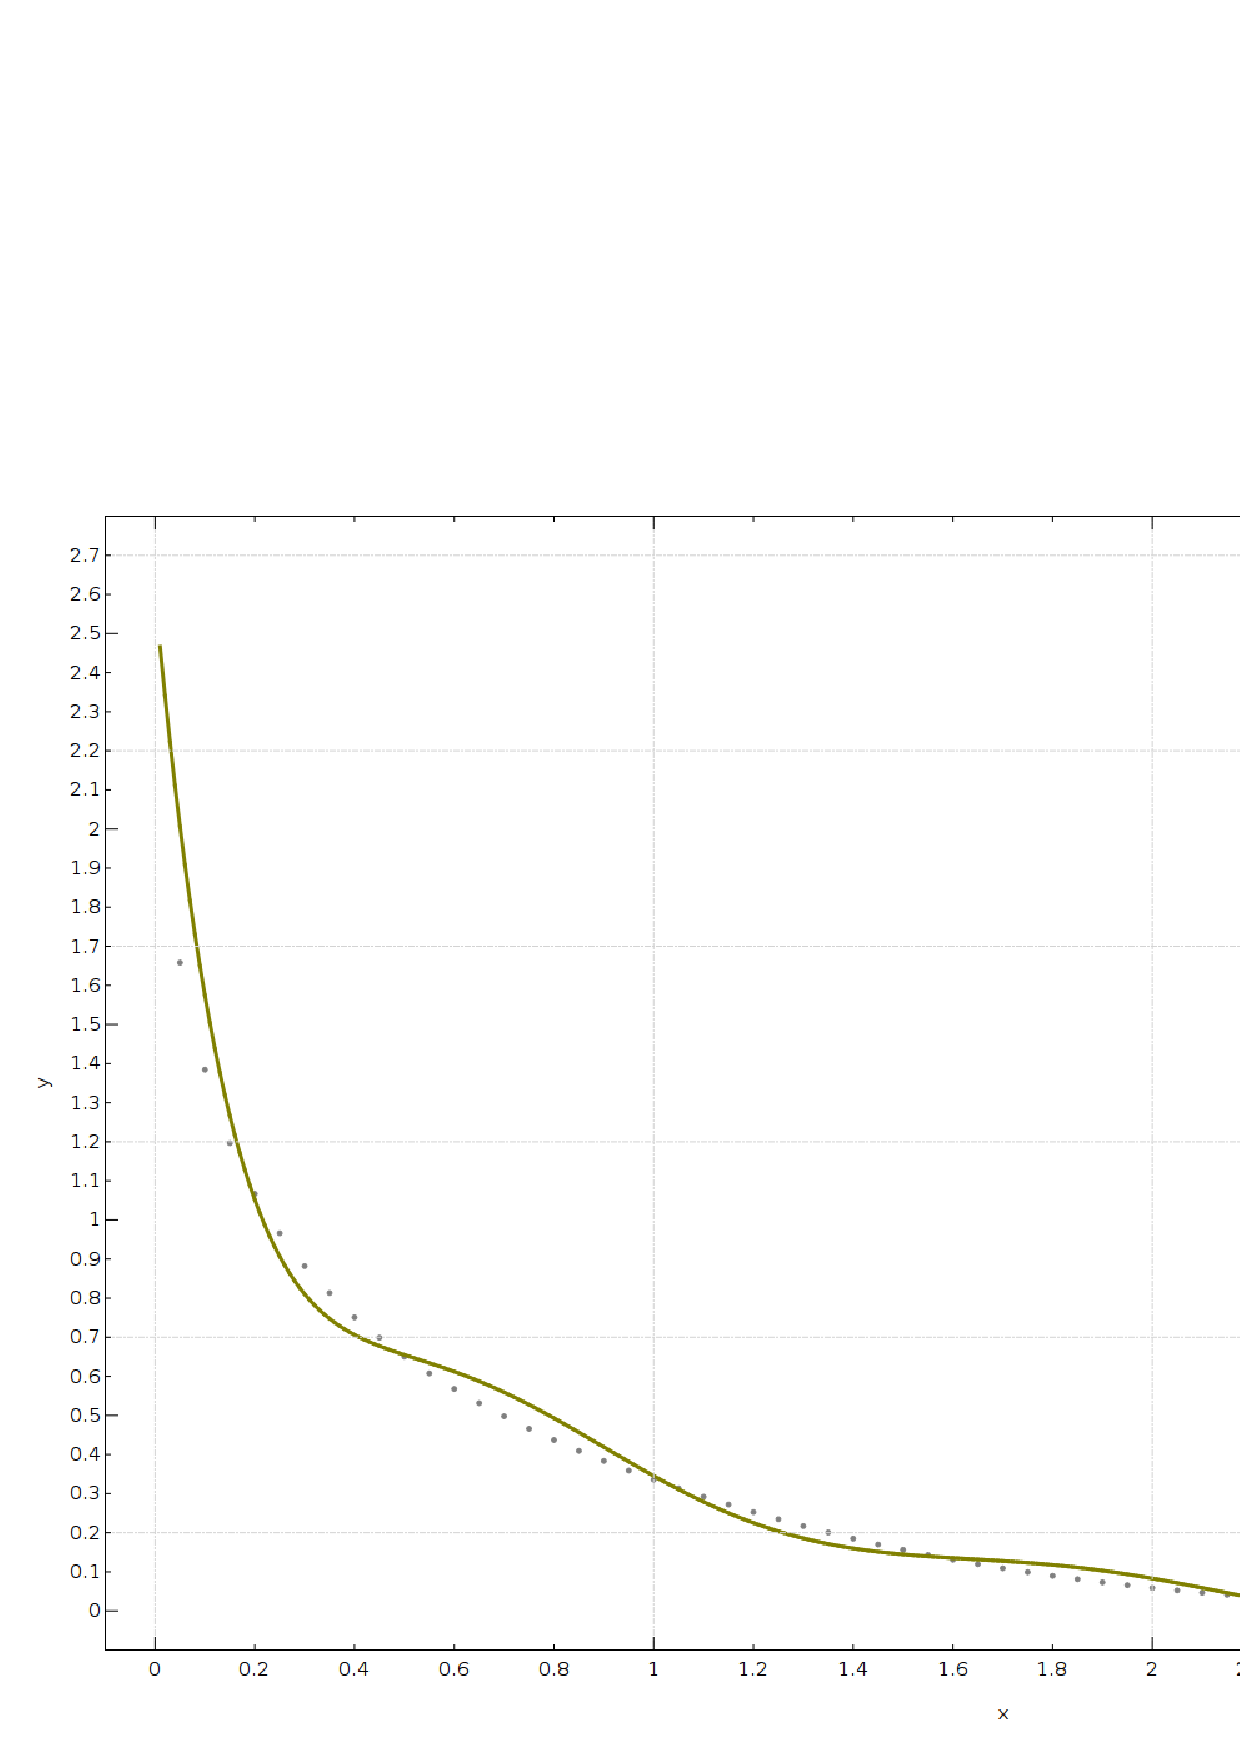
\includegraphics[width=16cm]{frgp_biznes1_op2_aproksymacja.pdf}
        \rule{35em}{0.5pt}
    \caption[Wykres przedstawiaj�cy niedok�adno�� aproksymacji funkcji g�sto�ci  \emph{ma�e} $\otimes$ \emph{nie bliskie 10 mln} ]{Wykres przedstawiaj�cy niedok�adno�� aproksymacji funkcji g�sto�ci \emph{ma�e} $\otimes$ \emph{nie bliskie 10 mln}}
    \label{wykres:frgp_biznes1_op2_aproksymacja}
\end{figure}

Ostatni� operacj� jest splecenie funkcji po�rednich, uzyskanych w operacjach \ref{equation:pierwsza_operacja_biznes1} oraz \ref{equation:druga_operacja_biznes1} : 
\begin{equation}
\label{equation:trzecia_operacja_biznes1}
gp_{DB1} = biznes1f1(x) \oplus biznes1f2(x) = fb10mln(p)\otimes D(p) \oplus fnb10mln(p)\otimes M(p), 
\end{equation}
o wzorach \ref{wzor:fgrp1_biznes1_op1_aproks_rownanie} i\ref{wzor:fgrp1_biznes1_op2_aproks_rownanie}. 
Wynik tego dzia�ania pokazany jest na wykresie \ref{wykres:frgp_biznes1_op3}, a niedok�adno�� aproksymacji na wykresie \ref{wykres:frgp_biznes1_op3_aproksymacja}. Wynikowa funkcja $gp_{DB1}$, ma wz�r:
\begin{equation}
\label{wzor:fgrp1_biznes1_op3_aproks_rownanie}
gp_{DB1} = \left\{ 
\begin{array}{l l}
\frac{2.5-1.5x + 0.2x^2 + 0.01x^3-0.007x^4 + 0.0006x^5 -0.001x^6}{0.9}, & \quad \text{ dla 3.18 $<$ $x$ $\leq$ 13.38}\\
  0, & \quad \text{ dla $-\infty$ $<$ $x$ $<$ 3.18 }\\
  0, & \quad \text{ dla 13.38 $<$ $x$ $<$ $\infty$}\\
\end{array} \right. . 
\end{equation}
\begin{figure}[ht]  
    \centering
    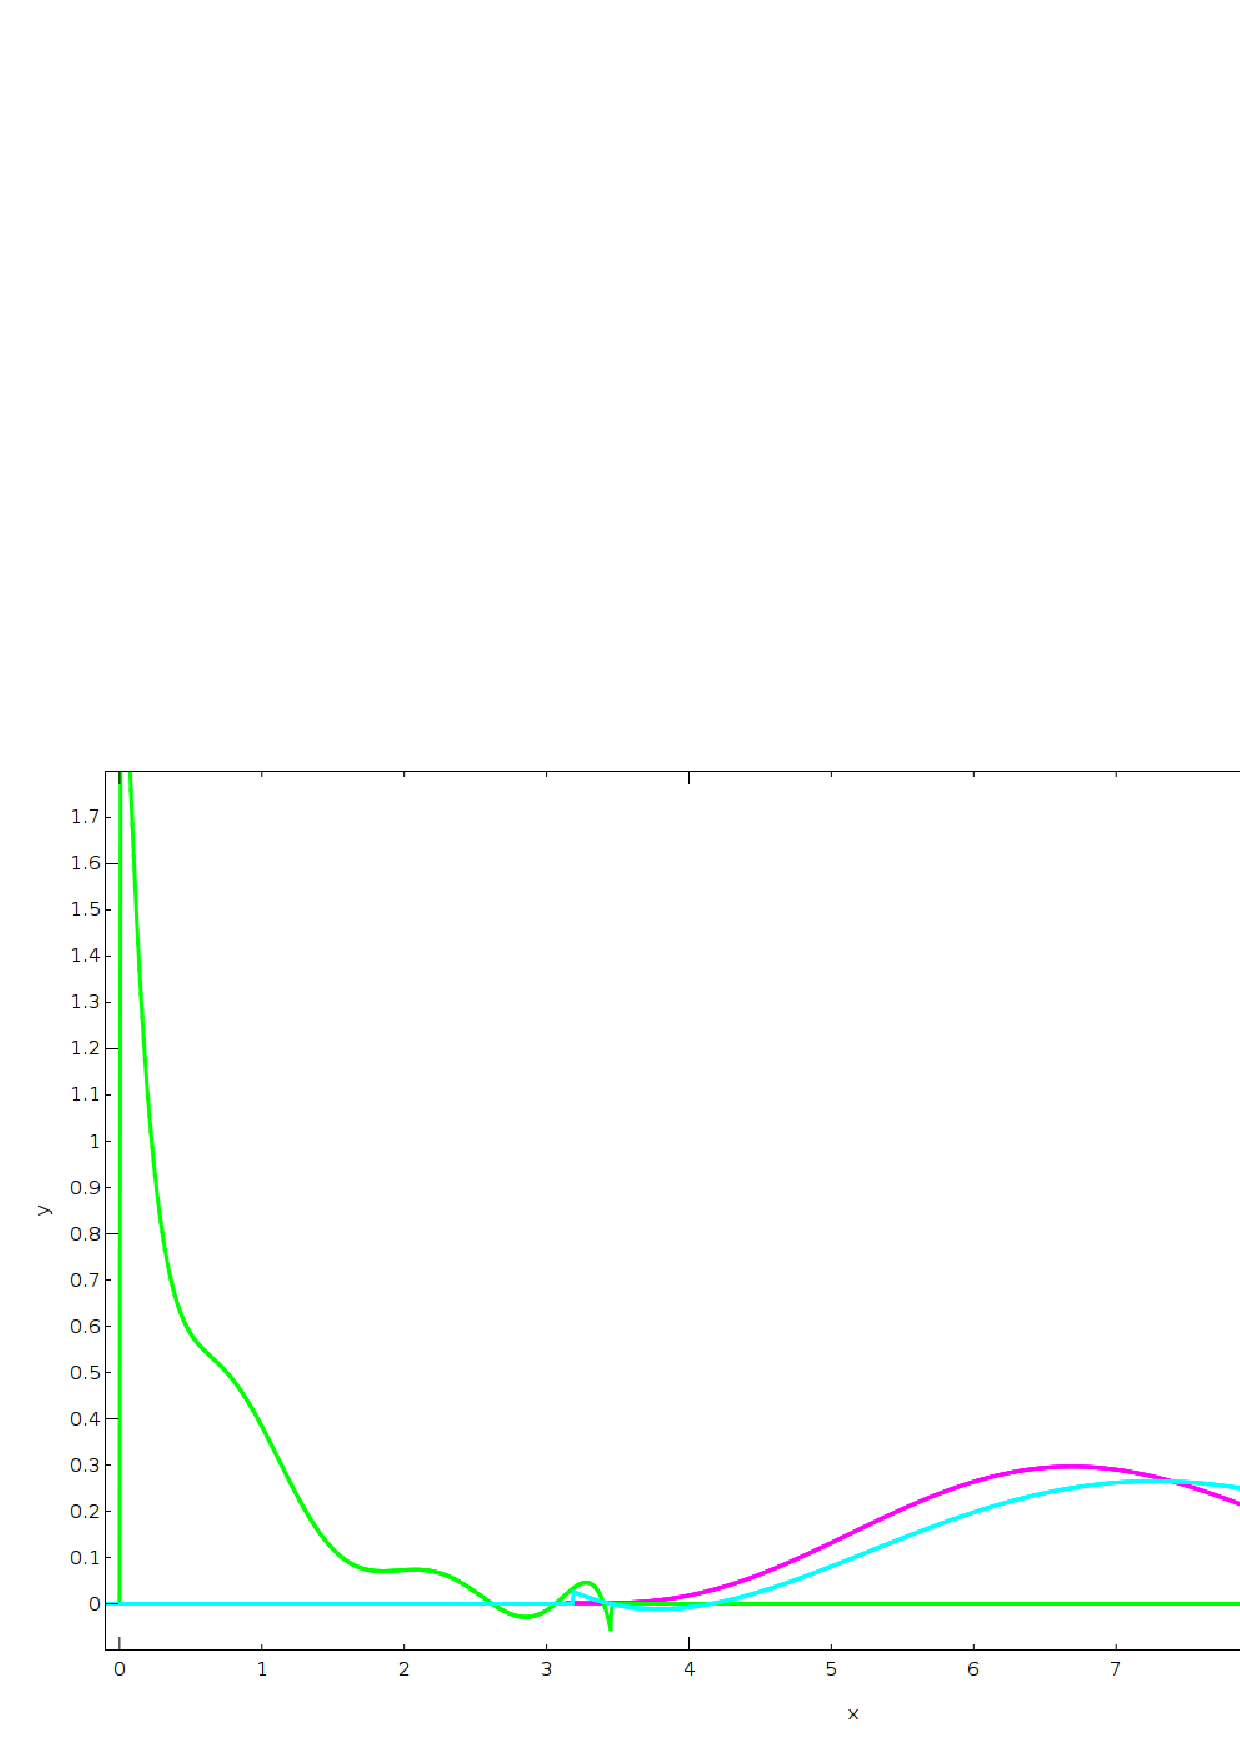
\includegraphics[width=16cm]{frgp_biznes1_op3.pdf}
        \rule{35em}{0.5pt}
    \caption[Wykres funkcji g�sto�ci $gp_{DB1}$ ]{Wykres funkcji g�sto�ci $gp_{DB1}$ }
    \label{wykres:frgp_biznes1_op3}
\end{figure}
\begin{figure}[ht]  
    \centering
    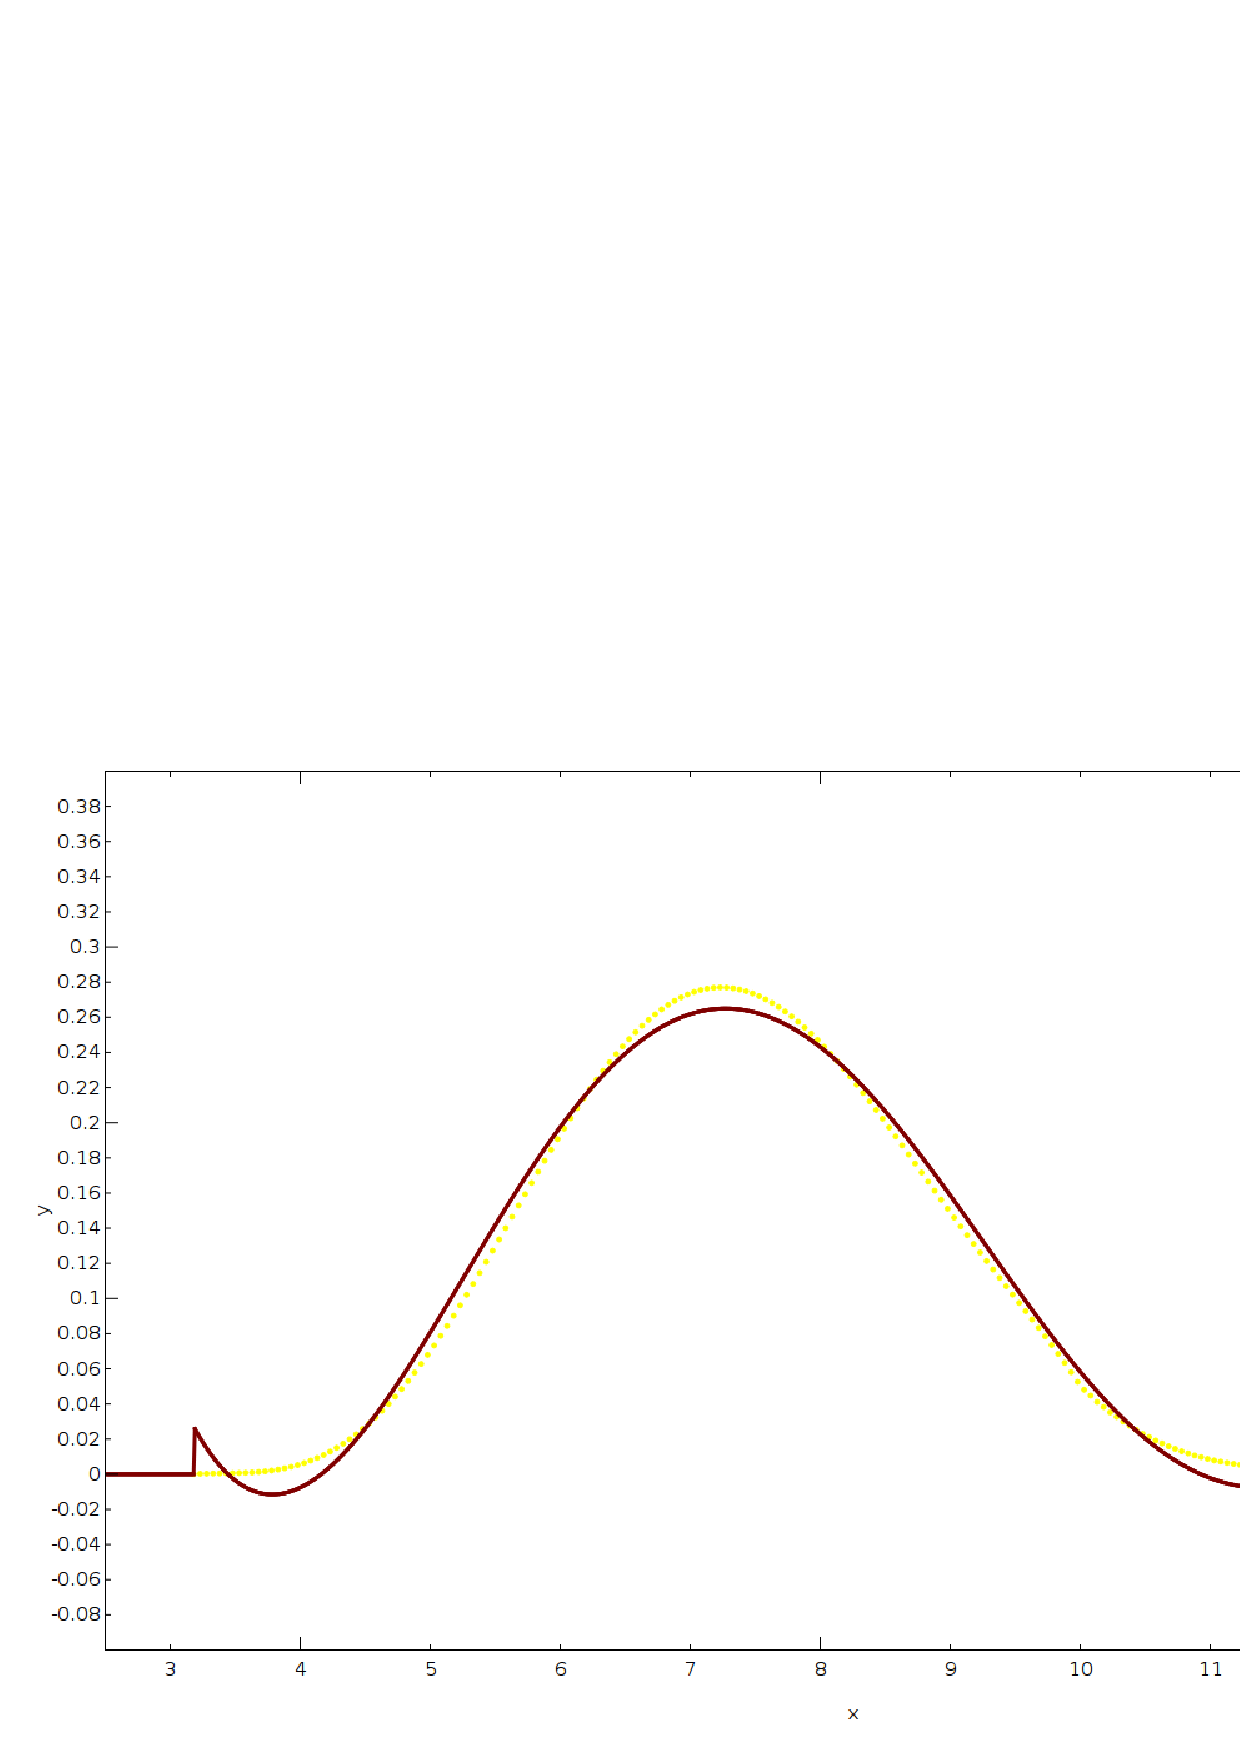
\includegraphics[width=16cm]{frgp_biznes1_op3_aproksymacja.pdf}
        \rule{35em}{0.5pt}
    \caption[Wykres przedstawiaj�cy niedok�adno�� aproksymacji funkcji g�sto�ci $gp_{DB1}$]{Wykres przedstawiaj�cy niedok�adno�� aproksymacji funkcji g�sto�ci $gp_{DB1}$}
    \label{wykres:frgp_biznes1_op3_aproksymacja}
\end{figure}

%%%%%%%%%%%%%%%%%%%%%%%%%%%%%%%%%%%%%%%%%%%%%%%%%%%%%%%%%%%%%%%%%%%%%%%%%%%%%%%%%%%%%%%%%%%%%%%%%%%%%%%%%%


\subsection{Funkcje rozk�adu g�sto�ci prawdopodobie�stwa dla biznesu drugiego}

Funkcja g�sto�ci rozk�adu prawdopodobie�stwa dla biznesu drugiego jest dana wzorem \ref{equation:funkcja_rozkladu_gest_prawd_biznes2}.
Tak jak w przypadku oblicze� funkcji g�sto�ci prawdopodobie�stwa dla biznesu pierwszego, tak w tym przypadku obliczenia zostan� podzielone na trzy operacje. 
Pierwszym dzia�aniem jest:
\begin{equation}
\label{equation:pierwsza_operacja_biznes2}
biznes2f1(x) = fnb20mln(p)\otimes D(p), 
\end{equation}
kt�ra zachodzi mi�dzy funkcjami rozk�ad�w g�sto�ci prawdopodobie�stwa dla kwantyfikator�w \emph{nie bliskie 20 mln} i \emph{du�e}.Wynik tego dzia�ania zosta� przedstawiony na wykresie \ref{wykres:frgp_biznes2_op1}, a niedok�adno�� odwzorowania zosta�a uwidoczniona na wykresie \ref{wykres:frgp_biznes2_op1_aproksymacja}. R�wnanie funkcji zosta�o przedstawione na wzorze \ref{wzor:fgrp1_biznes2_op1_aproks_rownanie}:
\begin{equation}
\label{wzor:fgrp1_biznes2_op1_aproks_rownanie}
biznes2f1(x) = \left\{ 
\begin{array}{l l}
 \frac{0.08+ 0.01x -0.01x^2 + 0.003x^3-0.0003x^4 }{0.98} & \quad \text{, dla 0.5 $<$ $x$ $\leq$ 15.35}\\
  0, & \quad \text{ dla $-\infty$ $<$ $x$ $<$ 0.5 }\\
  0, & \quad \text{ dla 15.35 $<$ $x$ $<$ $\infty$}\\
\end{array} \right. .
\end{equation}
\begin{figure}[ht]
    \centering
    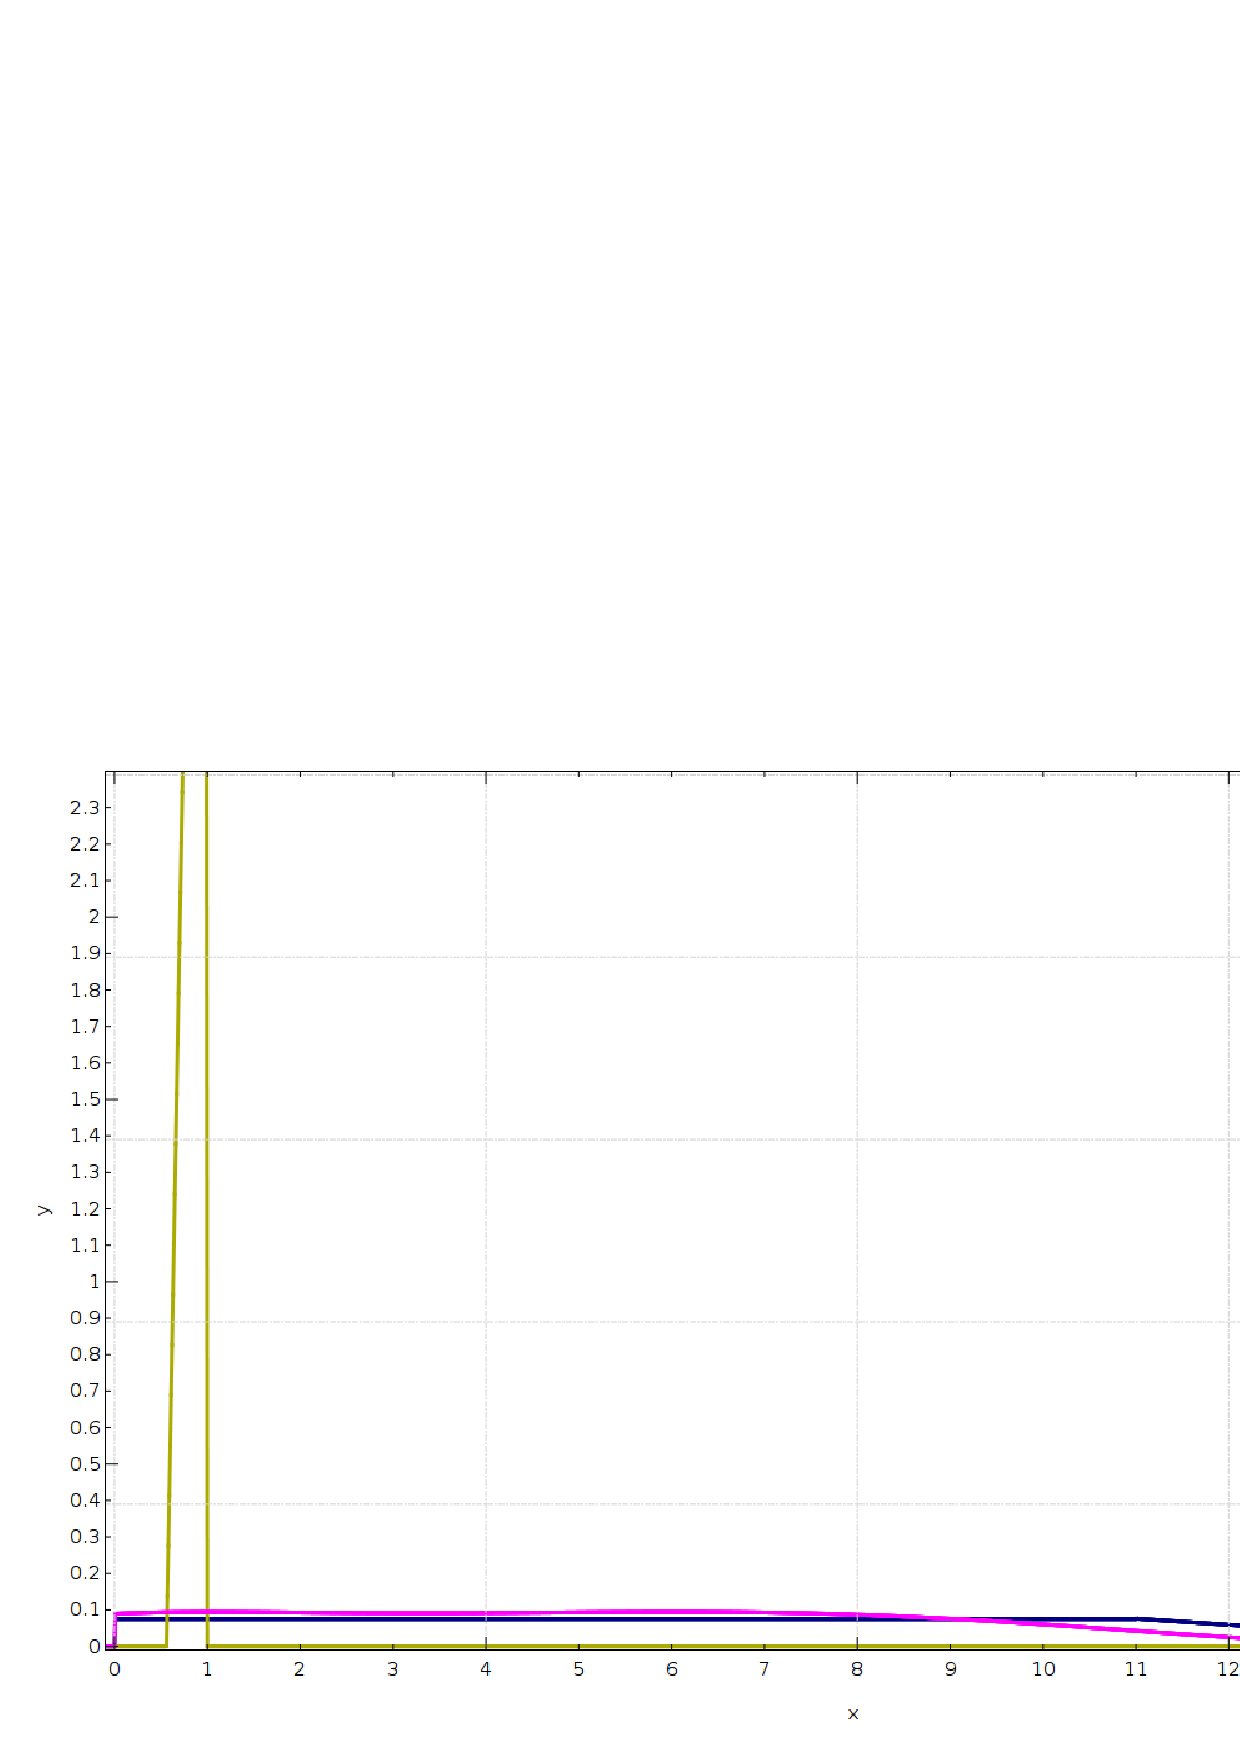
\includegraphics[width=16cm]{frgp_biznes2_op1.pdf}
        \rule{35em}{0.5pt}
    \caption[Wykres funkcji g�sto�ci dla kwantyfikator�w \emph{du�e} i \emph{nie bliskie 20 mln} oraz funkcji wynikowej dla operacji $\otimes$ mi�dzy nimi]{Wykres funkcji g�sto�ci dla kwantyfikator�w \emph{du�e} i \emph{nie bliskie 20 mln} oraz funkcji wynikowej dla operacji $\otimes$ mi�dzy nimi}
    \label{wykres:frgp_biznes2_op1}
\end{figure}
\begin{figure}[ht]  
    \centering
    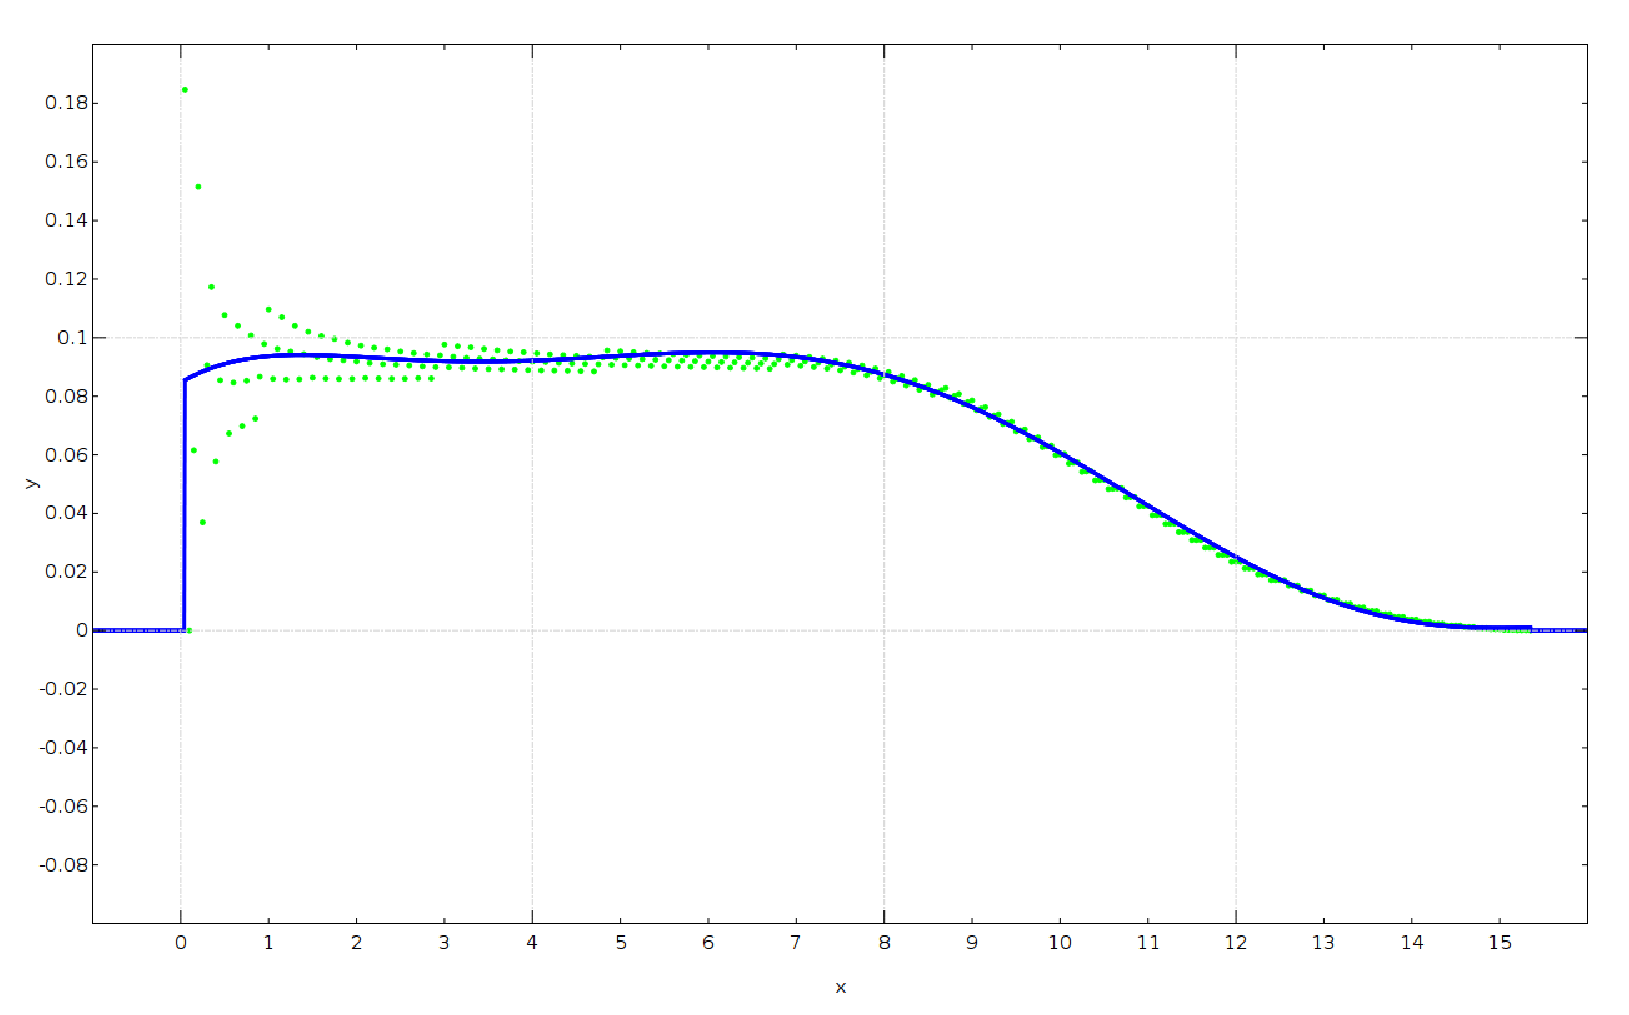
\includegraphics[width=16cm]{frgp_biznes2_op1_aproksymacja.eps}
        \rule{35em}{0.5pt}
    \caption[Wykres przedstawiaj�cy niedok�adno�� aproksymacji funkcji g�sto�ci \emph{nie bliskie 20 mln}$\otimes$\emph{du�e}]{Wykres przedstawiaj�cy niedok�adno�� aproksymacji funkcji g�sto�ci \emph{nie bliskie 10 mln}$\otimes$ \emph{du�e}}
    \label{wykres:frgp_biznes2_op1_aproksymacja}
\end{figure}
\newline

Nast�pnym dzia�aniem jest:
\begin{equation}
\label{equation:druga_operacja_biznes2}
biznes2f2(x) = fb20mln(p)\otimes M(p).
\end{equation}
Wynik tej operacji zosta� przedstawiony na wykresie \ref{wykres:frgp_biznes2_op2}. R�wnanie zaaproksymowanej funkcji zosta�o przedstawione na wzorze \ref{wzor:fgrp1_biznes2_op2_aproks_rownanie}, a niedok�adno�ci aproksymacji na wykresie \ref{wykres:frgp_biznes2_op2_aproksymacja}. 
\begin{figure}[ht]  
    \centering
    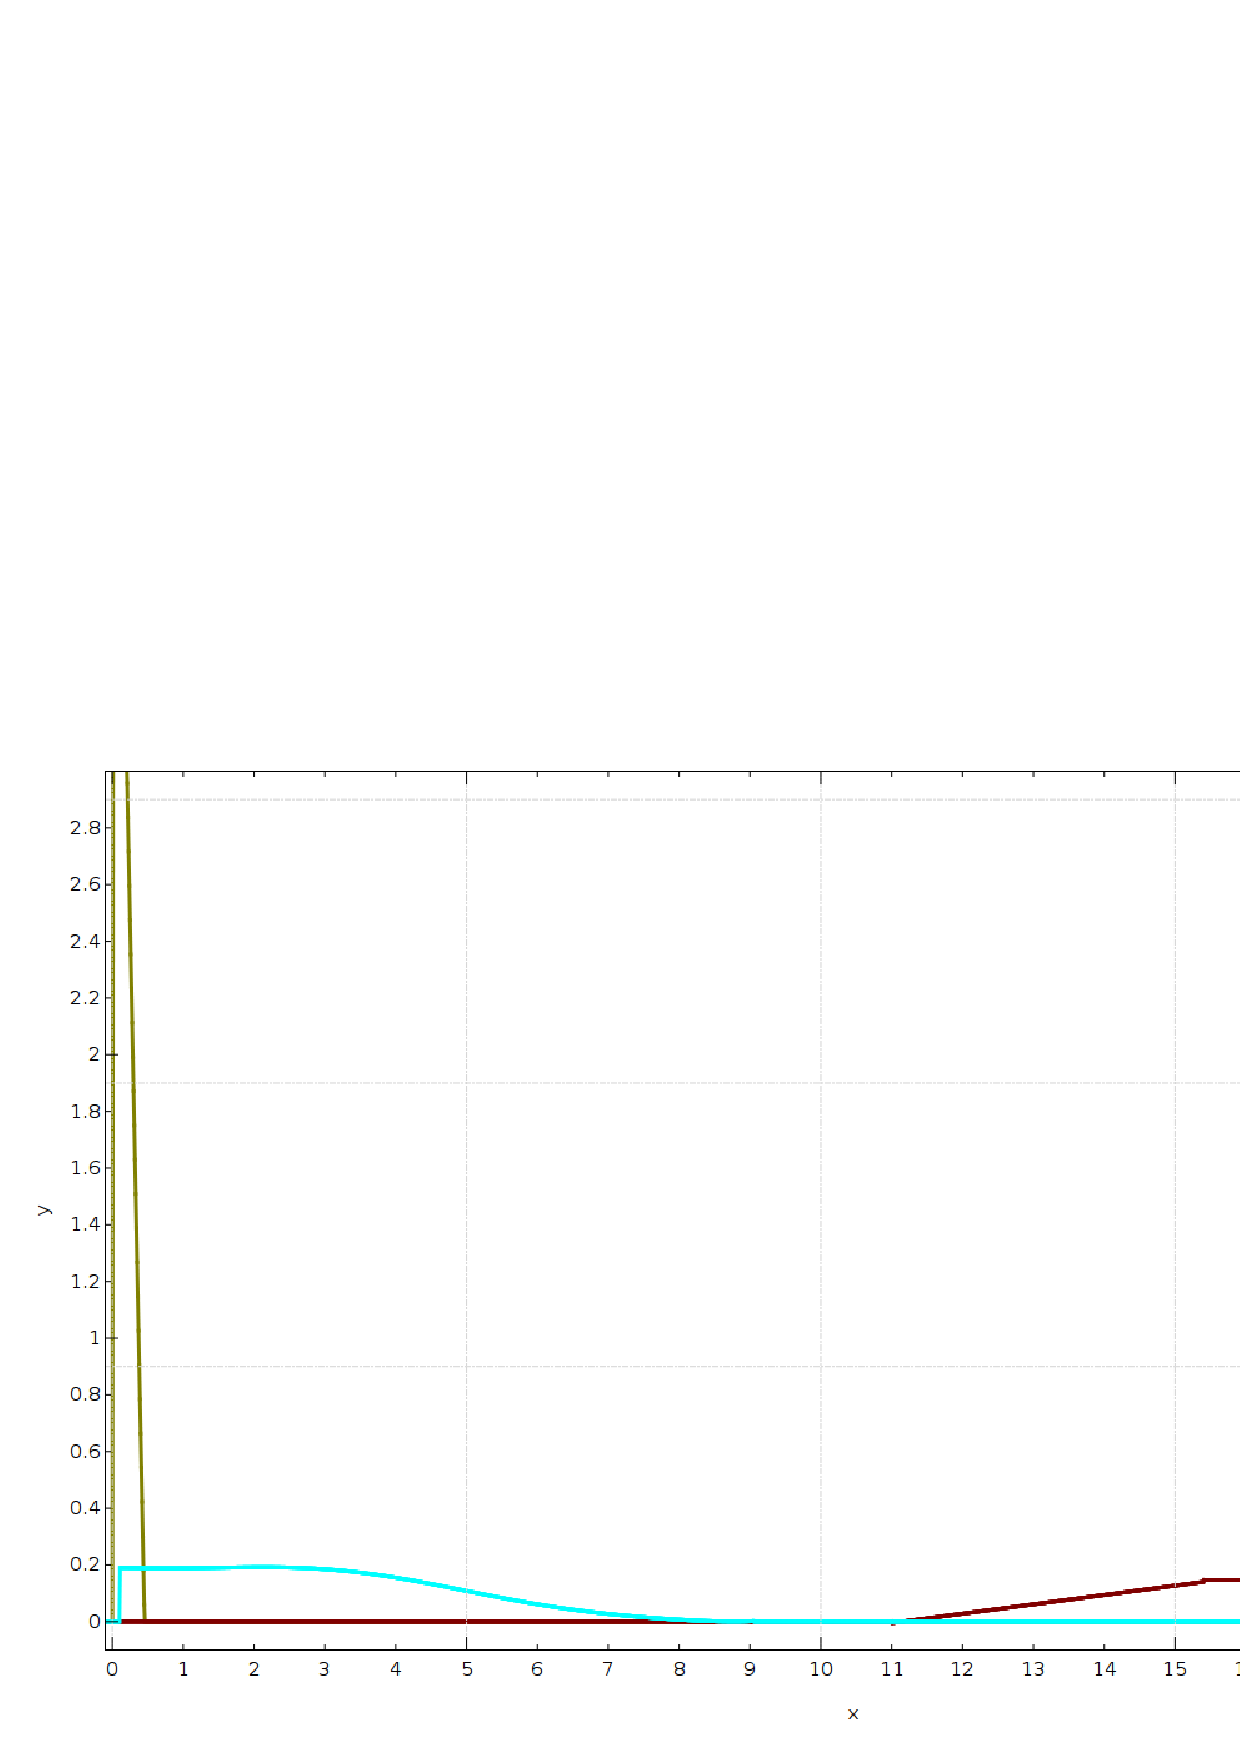
\includegraphics[width=16cm]{frgp_biznes2_op2.pdf}
        \rule{35em}{0.5pt}
    \caption[Wykres funkcji g�sto�ci dla kwantyfikator�w \emph{ma�e} i \emph{nie bliskie 10 mln} oraz funkcji wynikowej dla operacji $\otimes$ mi�dzy nimi]{Wykres funkcji g�sto�ci dla kwantyfikator�w \emph{ma�e} i \emph{nie bliskie 10 mln} oraz funkcji wynikowej dla operacji $\otimes$ mi�dzy nimi}
    \label{wykres:frgp_biznes2_op2}
\end{figure}
\begin{equation}
\label{wzor:fgrp1_biznes2_op2_aproks_rownanie}
biznes1f2(x) = \left\{ 
\begin{array}{l l}
 \frac{0.1-0.02x + 0.03x^2 -0.01x^3 + 0.001x^4}{0.95} & \quad \text{ dla 0.1 $<$ $x$ $\leq$ 9.05}\\
  0, & \quad \text{ dla $-\infty$ $<$ $x$ $<$ 0.1 }\\
  0, & \quad \text{ dla 9.05 $<$ $x$ $<$ $\infty$}\\
\end{array} \right.
\end{equation}
\begin{figure}[ht]  
    \centering
    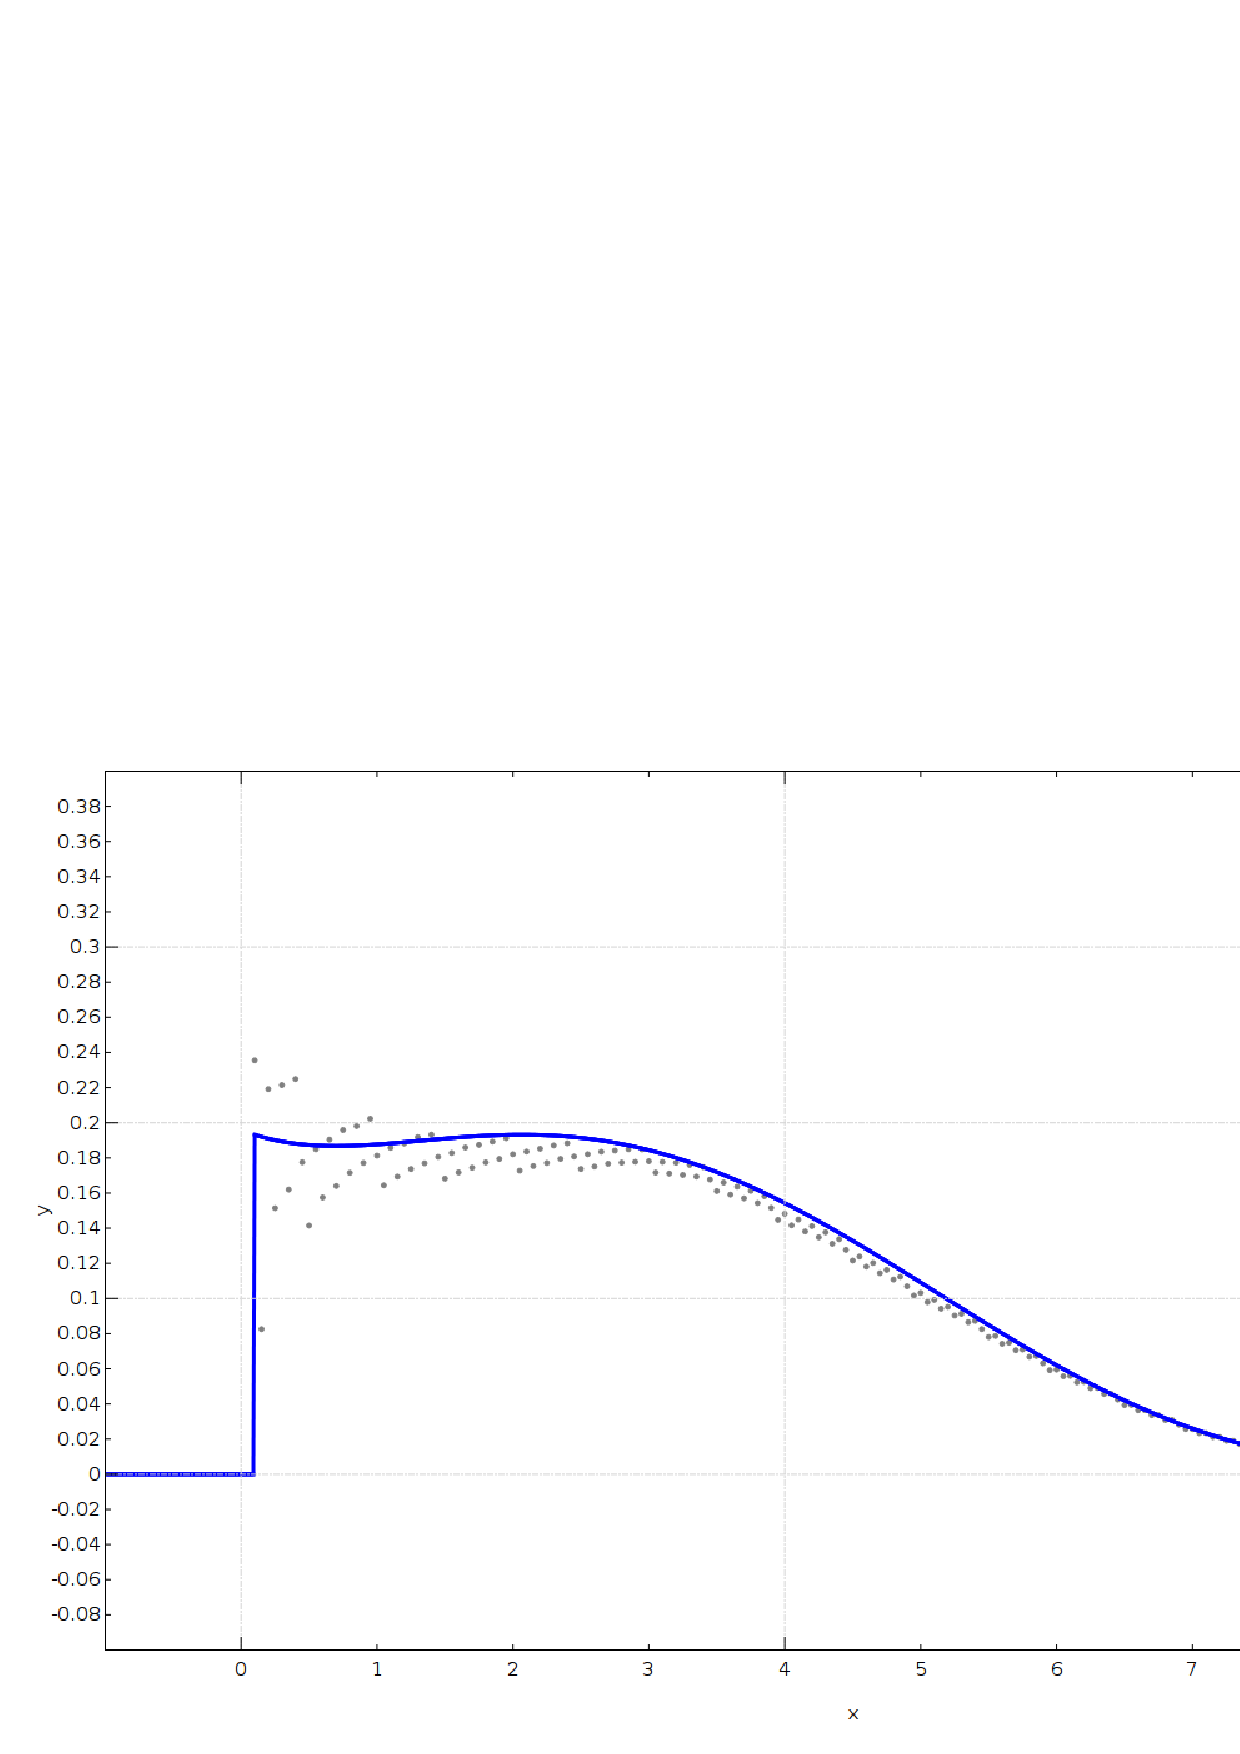
\includegraphics[width=16cm]{frgp_biznes2_op2_aproksymacja.pdf}
        \rule{35em}{0.5pt}
    \caption[Wykres przedstawiaj�cy niedok�adno�� aproksymacji funkcji g�sto�ci  \emph{ma�e} $\otimes$ \emph{nie bliskie 10 mln} ]{Wykres przedstawiaj�cy niedok�adno�� aproksymacji funkcji g�sto�ci \emph{ma�e} $\otimes$ \emph{nie bliskie 10 mln}}
    \label{wykres:frgp_biznes2_op2_aproksymacja}
\end{figure}
% 

Ostatni� operacj� jest splecenie funkcji po�rednich, uzyskanych w operacjach \ref{equation:pierwsza_operacja_biznes2} oraz \ref{equation:druga_operacja_biznes2} : 
\begin{equation}
\label{equation:trzecia_operacja_biznes2}
gp_{DB2} = biznes2f1(x) \oplus biznes2f2(x) = fnb20mln(p)\otimes D(p) \oplus fb20mln(p)\otimes M(p), 
\end{equation}
o wzorach \ref{wzor:fgrp1_biznes2_op1_aproks_rownanie} i\ref{wzor:fgrp1_biznes2_op2_aproks_rownanie}. 
Wynik tego dzia�ania pokazany jest na wykresie \ref{wykres:frgp_biznes2_op3}, a niedok�adno�� aproksymacji na wykresie \ref{wykres:frgp_biznes2_op3_aproksymacja}. Wynikowa funkcja $gp_{DB2}$, ma wz�r:
\begin{equation}
\label{wzor:fgrp1_biznes2_op3_aproks_rownanie}
gp_{DB2} = \left\{ 
\begin{array}{l l}
\frac{-0.001+ 0.01x + 0.001x^2 + -0.0003x^3 + 1.37708e-05*x^4}{1.0002}, & \quad \text{ dla 0.25 $<$ $x$ $\leq$ 24.35 }\\
  0, & \quad \text{ dla $-\infty$ $<$ $x$ $<$ 3.18 }\\
  0, & \quad \text{ dla 13.38 $<$ $x$ $<$ $\infty$}\\
\end{array} \right. . 
\end{equation}
\begin{figure}[ht]  
    \centering
    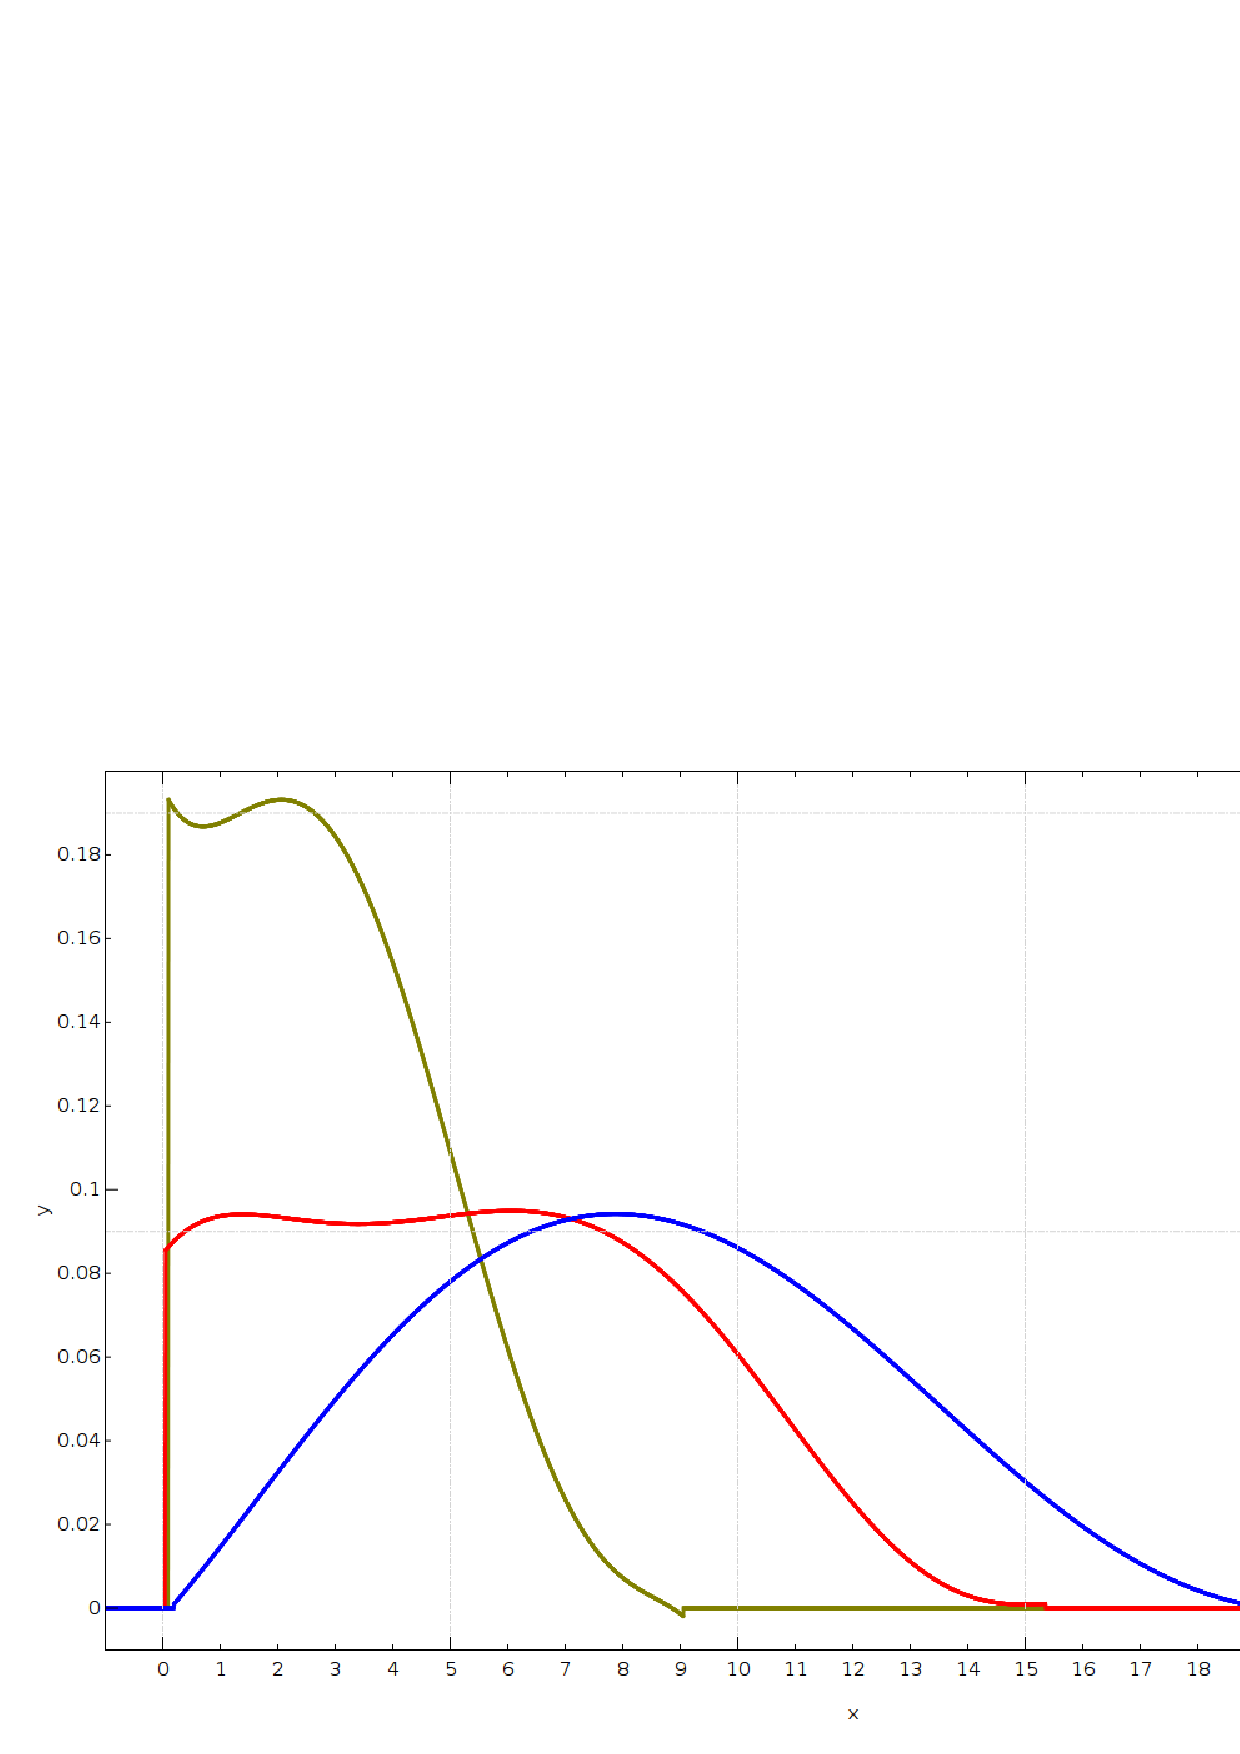
\includegraphics[width=16cm]{frgp_biznes2_op3.pdf}
        \rule{35em}{0.5pt}
    \caption[Wykres funkcji g�sto�ci $gp_{DB2}$ ]{Wykres funkcji g�sto�ci $gp_{DB2}$ }
    \label{wykres:frgp_biznes2_op3}
\end{figure}
\begin{figure}[ht]  
    \centering
    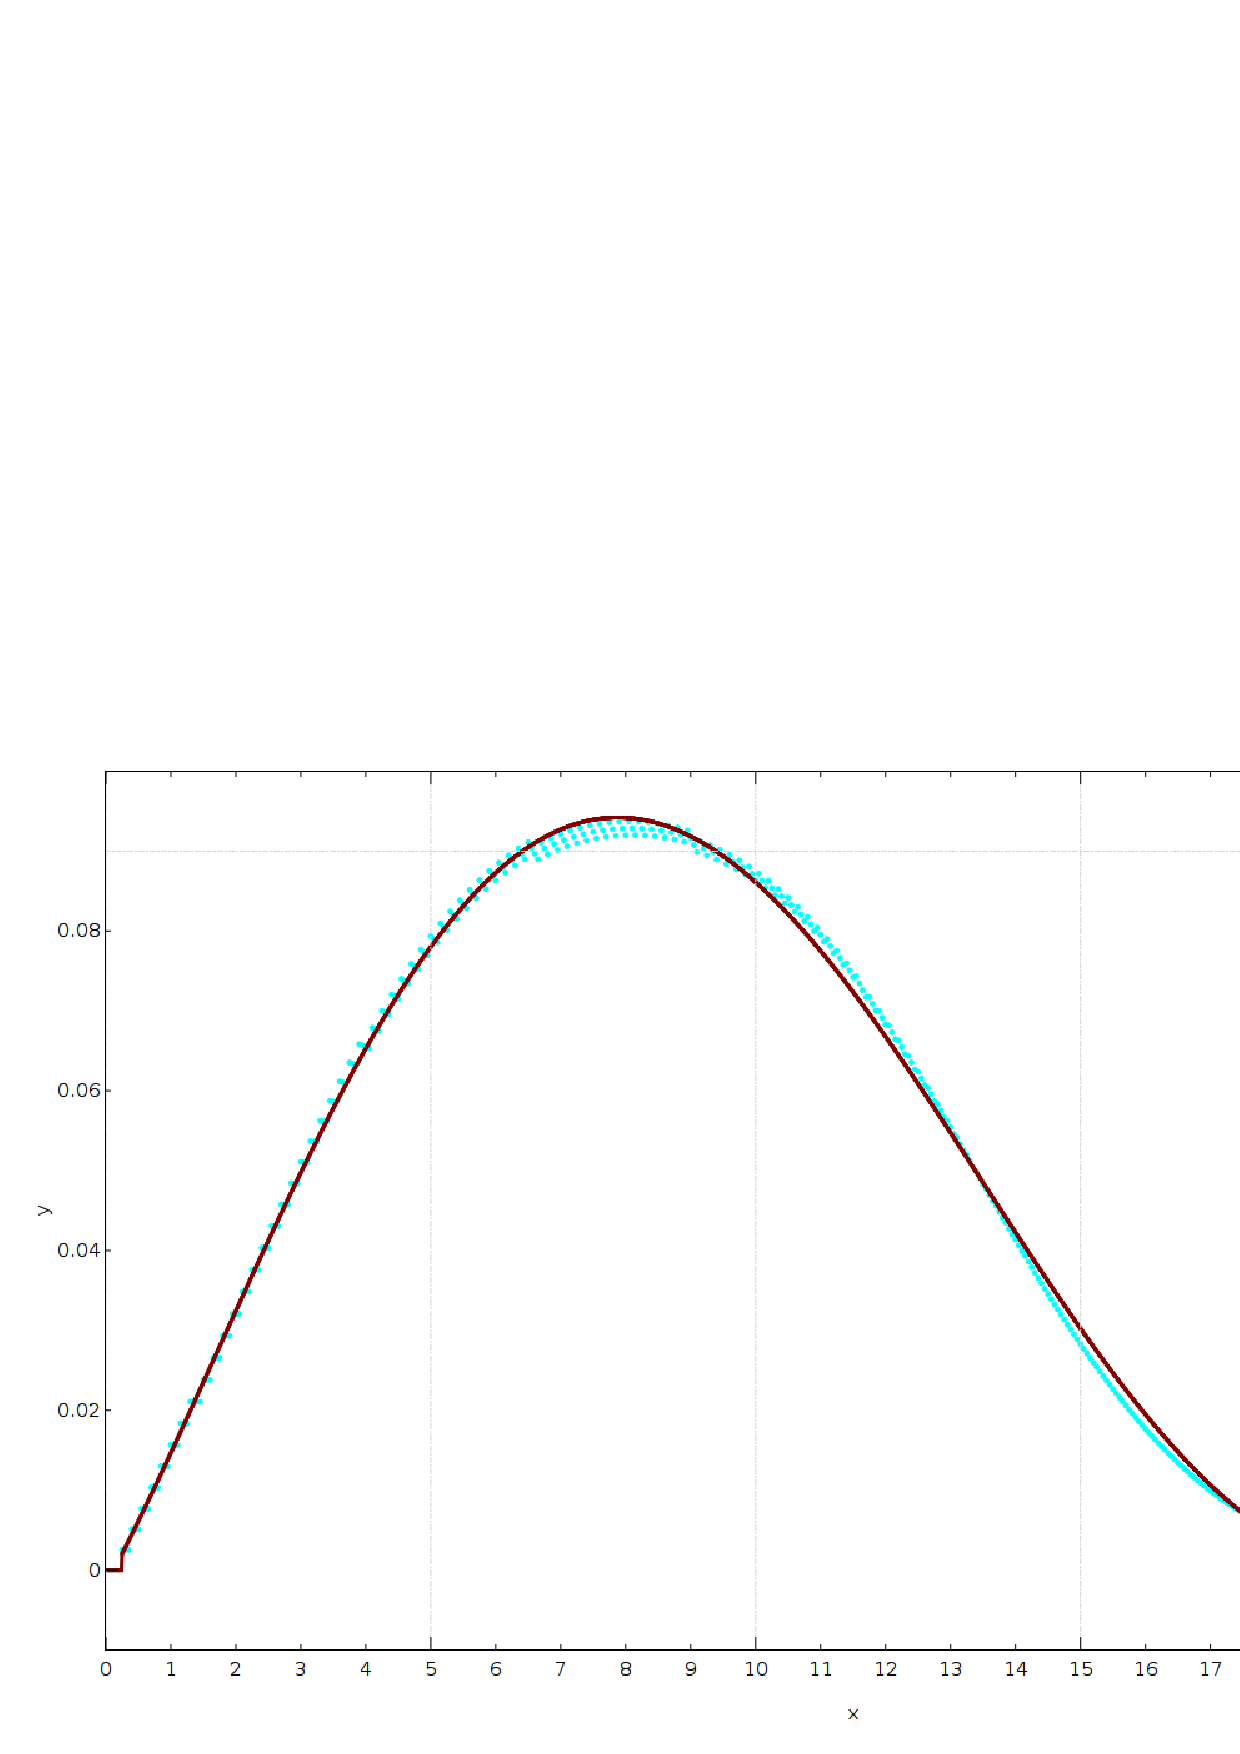
\includegraphics[width=16cm]{frgp_biznes2_op3_aproksymacja.pdf}
        \rule{35em}{0.5pt}
    \caption[Wykres przedstawiaj�cy niedok�adno�� aproksymacji funkcji g�sto�ci $gp_{DB2}$]{Wykres przedstawiaj�cy niedok�adno�� aproksymacji funkcji g�sto�ci $gp_{DB2}$}
    \label{wykres:frgp_biznes2_op3_aproksymacja}    
\end{figure}
\subsection{Warto�ci oczekiwane i b��d}
Z funkcji rozk�adu g�sto�ci prawdopodobie�stwa biznesu pierwszego, danej wzorem \ref{wzor:fgrp1_biznes1_op3_aproks_rownanie}, policzona warto�� oczekiwana wynosi $\approx$ 7.4, natomiast z funkcji rozk�adu g�sto�ci prawdopodobie�stwa biznesu drugiego, danej wzorem \ref{wzor:fgrp1_biznes1_op3_aproks_rownanie}, wyliczona warto�� oczekiwana wynosi $\approx$ 8.46. Na rysunku \ref{wykres:funkcje_rozkladu} przedstawiono oba funkcje rozk�ad�w g�sto�ci dla obu biznes�w.
\begin{figure}[ht]  
    \centering
    \includegraphics[width=16cm]{funkcje_rozkladu.pdf}
        \rule{35em}{0.5pt}
    \caption[Wykres przedstawiaj�cy niedok�adno�� aproksymacji funkcji g�sto�ci $gp_{DB2}$]{Wykres przedstawiaj�cy niedok�adno�� aproksymacji funkcji g�sto�ci $gp_{DB2}$}
    \label{wykres:funkcje_rozkladu}    
\end{figure}
\newline
Przedstawione wy�ej warto�ci s� warto�ciami u�rednionymi. Zale�nie od wyboru stopnia wielomian�w, kt�rymi aproksymowali�my wynikowe funkcje, warto�� oczekiwana obu ko�cowych rozk�ad�w ulega�a zmianie. Warto�� oczekiwana biznesu pierwszego zawsze nale�a�a do przedzia�u $[7.34,7.4]$, natomiast dla biznesu drugiego $[8.38,8.55]$. B��d wyniku dla pierwszego biznesu wynosi� zatem $\approx$ 1 \% i by� taki sam jak dla biznesu drugiego. 
\newline
B��d na takim poziomie nie wp�ywa na ko�cowy wynik. 
\subsection{Odpowied� na problem dw�ch biznes�w}

Ze statystycznego punktu widzenia, zdecydowanie lepiej jest wybra� biznes drugi, poniewa� warto�� oczekiwana dochodu z niego jest wy�sza $\approx$ 1 mln z�otych. 



\addtocontents{toc}{\vspace{2em}}

\appendix % Cue to tell LaTeX that the following 'chapters' are Appendices


\addtocontents{toc}{\vspace{2em}}  % Add a gap in the Contents, for aesthetics
\backmatter

%% ----------------------------------------------------------------
\label{Bibliografia}
\lhead{\emph{Bibliografia}}  % Change the left side page header to "Bibliography"
\bibliographystyle{plplain}  % Use the "unsrtnat" BibTeX style for formatting the Bibliography
\bibliography{Bibliography}  % The references (bibliography) information are stored in the file named "Bibliography.bib"

\end{document}  % The End
%% ----------------------------------------------------------------
